\documentclass[]{book}
\usepackage{lmodern}
\usepackage{amssymb,amsmath}
\usepackage{ifxetex,ifluatex}
\usepackage{fixltx2e} % provides \textsubscript
\ifnum 0\ifxetex 1\fi\ifluatex 1\fi=0 % if pdftex
  \usepackage[T1]{fontenc}
  \usepackage[utf8]{inputenc}
\else % if luatex or xelatex
  \ifxetex
    \usepackage{mathspec}
  \else
    \usepackage{fontspec}
  \fi
  \defaultfontfeatures{Ligatures=TeX,Scale=MatchLowercase}
\fi
% use upquote if available, for straight quotes in verbatim environments
\IfFileExists{upquote.sty}{\usepackage{upquote}}{}
% use microtype if available
\IfFileExists{microtype.sty}{%
\usepackage{microtype}
\UseMicrotypeSet[protrusion]{basicmath} % disable protrusion for tt fonts
}{}
\usepackage[margin=1in]{geometry}
\usepackage{hyperref}
\hypersetup{unicode=true,
            pdftitle={Predictive Models: Visualisation, Exploration and Explanation},
            pdfauthor={Przemyslaw Biecek and Tomasz Burzykowski},
            pdfborder={0 0 0},
            breaklinks=true}
\urlstyle{same}  % don't use monospace font for urls
\usepackage{natbib}
\bibliographystyle{apalike}
\usepackage{color}
\usepackage{fancyvrb}
\newcommand{\VerbBar}{|}
\newcommand{\VERB}{\Verb[commandchars=\\\{\}]}
\DefineVerbatimEnvironment{Highlighting}{Verbatim}{commandchars=\\\{\}}
% Add ',fontsize=\small' for more characters per line
\usepackage{framed}
\definecolor{shadecolor}{RGB}{248,248,248}
\newenvironment{Shaded}{\begin{snugshade}}{\end{snugshade}}
\newcommand{\AlertTok}[1]{\textcolor[rgb]{0.94,0.16,0.16}{#1}}
\newcommand{\AnnotationTok}[1]{\textcolor[rgb]{0.56,0.35,0.01}{\textbf{\textit{#1}}}}
\newcommand{\AttributeTok}[1]{\textcolor[rgb]{0.77,0.63,0.00}{#1}}
\newcommand{\BaseNTok}[1]{\textcolor[rgb]{0.00,0.00,0.81}{#1}}
\newcommand{\BuiltInTok}[1]{#1}
\newcommand{\CharTok}[1]{\textcolor[rgb]{0.31,0.60,0.02}{#1}}
\newcommand{\CommentTok}[1]{\textcolor[rgb]{0.56,0.35,0.01}{\textit{#1}}}
\newcommand{\CommentVarTok}[1]{\textcolor[rgb]{0.56,0.35,0.01}{\textbf{\textit{#1}}}}
\newcommand{\ConstantTok}[1]{\textcolor[rgb]{0.00,0.00,0.00}{#1}}
\newcommand{\ControlFlowTok}[1]{\textcolor[rgb]{0.13,0.29,0.53}{\textbf{#1}}}
\newcommand{\DataTypeTok}[1]{\textcolor[rgb]{0.13,0.29,0.53}{#1}}
\newcommand{\DecValTok}[1]{\textcolor[rgb]{0.00,0.00,0.81}{#1}}
\newcommand{\DocumentationTok}[1]{\textcolor[rgb]{0.56,0.35,0.01}{\textbf{\textit{#1}}}}
\newcommand{\ErrorTok}[1]{\textcolor[rgb]{0.64,0.00,0.00}{\textbf{#1}}}
\newcommand{\ExtensionTok}[1]{#1}
\newcommand{\FloatTok}[1]{\textcolor[rgb]{0.00,0.00,0.81}{#1}}
\newcommand{\FunctionTok}[1]{\textcolor[rgb]{0.00,0.00,0.00}{#1}}
\newcommand{\ImportTok}[1]{#1}
\newcommand{\InformationTok}[1]{\textcolor[rgb]{0.56,0.35,0.01}{\textbf{\textit{#1}}}}
\newcommand{\KeywordTok}[1]{\textcolor[rgb]{0.13,0.29,0.53}{\textbf{#1}}}
\newcommand{\NormalTok}[1]{#1}
\newcommand{\OperatorTok}[1]{\textcolor[rgb]{0.81,0.36,0.00}{\textbf{#1}}}
\newcommand{\OtherTok}[1]{\textcolor[rgb]{0.56,0.35,0.01}{#1}}
\newcommand{\PreprocessorTok}[1]{\textcolor[rgb]{0.56,0.35,0.01}{\textit{#1}}}
\newcommand{\RegionMarkerTok}[1]{#1}
\newcommand{\SpecialCharTok}[1]{\textcolor[rgb]{0.00,0.00,0.00}{#1}}
\newcommand{\SpecialStringTok}[1]{\textcolor[rgb]{0.31,0.60,0.02}{#1}}
\newcommand{\StringTok}[1]{\textcolor[rgb]{0.31,0.60,0.02}{#1}}
\newcommand{\VariableTok}[1]{\textcolor[rgb]{0.00,0.00,0.00}{#1}}
\newcommand{\VerbatimStringTok}[1]{\textcolor[rgb]{0.31,0.60,0.02}{#1}}
\newcommand{\WarningTok}[1]{\textcolor[rgb]{0.56,0.35,0.01}{\textbf{\textit{#1}}}}
\usepackage{longtable,booktabs}
\usepackage{graphicx,grffile}
\makeatletter
\def\maxwidth{\ifdim\Gin@nat@width>\linewidth\linewidth\else\Gin@nat@width\fi}
\def\maxheight{\ifdim\Gin@nat@height>\textheight\textheight\else\Gin@nat@height\fi}
\makeatother
% Scale images if necessary, so that they will not overflow the page
% margins by default, and it is still possible to overwrite the defaults
% using explicit options in \includegraphics[width, height, ...]{}
\setkeys{Gin}{width=\maxwidth,height=\maxheight,keepaspectratio}
\IfFileExists{parskip.sty}{%
\usepackage{parskip}
}{% else
\setlength{\parindent}{0pt}
\setlength{\parskip}{6pt plus 2pt minus 1pt}
}
\setlength{\emergencystretch}{3em}  % prevent overfull lines
\providecommand{\tightlist}{%
  \setlength{\itemsep}{0pt}\setlength{\parskip}{0pt}}
\setcounter{secnumdepth}{5}
% Redefines (sub)paragraphs to behave more like sections
\ifx\paragraph\undefined\else
\let\oldparagraph\paragraph
\renewcommand{\paragraph}[1]{\oldparagraph{#1}\mbox{}}
\fi
\ifx\subparagraph\undefined\else
\let\oldsubparagraph\subparagraph
\renewcommand{\subparagraph}[1]{\oldsubparagraph{#1}\mbox{}}
\fi

%%% Use protect on footnotes to avoid problems with footnotes in titles
\let\rmarkdownfootnote\footnote%
\def\footnote{\protect\rmarkdownfootnote}

%%% Change title format to be more compact
\usepackage{titling}

% Create subtitle command for use in maketitle
\newcommand{\subtitle}[1]{
  \posttitle{
    \begin{center}\large#1\end{center}
    }
}

\setlength{\droptitle}{-2em}

  \title{Predictive Models: Visualisation, Exploration and Explanation}
    \pretitle{\vspace{\droptitle}\centering\huge}
  \posttitle{\par}
    \author{Przemyslaw Biecek and Tomasz Burzykowski}
    \preauthor{\centering\large\emph}
  \postauthor{\par}
      \predate{\centering\large\emph}
  \postdate{\par}
    \date{2018-09-23}

\usepackage{booktabs}

\usepackage{amsthm}
\newtheorem{theorem}{Theorem}[chapter]
\newtheorem{lemma}{Lemma}[chapter]
\theoremstyle{definition}
\newtheorem{definition}{Definition}[chapter]
\newtheorem{corollary}{Corollary}[chapter]
\newtheorem{proposition}{Proposition}[chapter]
\theoremstyle{definition}
\newtheorem{example}{Example}[chapter]
\theoremstyle{definition}
\newtheorem{exercise}{Exercise}[chapter]
\theoremstyle{remark}
\newtheorem*{remark}{Remark}
\newtheorem*{solution}{Solution}
\begin{document}
\maketitle

{
\setcounter{tocdepth}{1}
\tableofcontents
}
\hypertarget{introduction}{%
\chapter{Introduction}\label{introduction}}

Predictive models are used to automatically guess (statisticians would
say: estimate) one interesting variable based on other variables. Think
about prediction of sales based on historical data, prediction of risk
of heart disease based on demographic factors, prediction of political
attitudes based on facebook comments.

There is a lot of very interesting applications.

\textbf{NOTE} The use of word \emph{guess} is intended as the word
\emph{prediction} may result in false impression that the prediction is
accurate. Yet in many cases it is not. And if we are going to be
sceptical about these models it is better to use the words \emph{guess}.

Machine Learning models have a wide range of applications in
classification or regression problems. Due to the increasing
computational power of computers and complexity of data sources, ML
models are becoming more and more sophisticated. Models created with the
use of techniques such as boosting or bagging of neural networks are
parametrized by thousands of coefficients. They are obscure; it is hard
to trace the link between input variables and model outcomes - in fact
they are treated as black boxes. They are used because of their
elasticity and high performance, but their deficiency in
interpretability is one of their weakest sides.

In many applications we need to know, understand or prove how the input
variables are used in the model. We need to know the impact of
particular variables on the final model predictions. Thus we need tools
that extract useful information from thousands of model parameters.

\textbf{This book is about}

\begin{itemize}
\tightlist
\item
  We present techniques to examine particular predictions from ML
  models. In this book you will find theory and examples that explains
  model locally like break down, ceteris paribus, LIME or Shapley.
\item
  We present techniques to examine fully trained ML models as a whole.
  In this book you will find theory and examples that explains model
  globally like Partial Dependency Plots, Variable Importance Plots and
  others.
\item
  We present tools and methods for model comparison.
\end{itemize}

\textbf{This book is NOT about.}

\begin{itemize}
\tightlist
\item
  We do not focus on any specific model. Presented techniques are model
  agnostic and do not have any assumptions related to model structure.
\item
  We do not focus on the data exploration. There are very good books and
  techniques related to this, like R for Data Science
  \url{http://r4ds.had.co.nz/} or TODO
\item
  We do not focus on the process of model building. There are also very
  good books about this, see An Introduction to Statistical Learning by
  Gareth James, Daniela Witten, Trevor Hastie and Robert Tibshirani
  \url{http://www-bcf.usc.edu/~gareth/ISL/} or TODO
\item
  We do not focus on particular tools for model building, see Applied
  Predictive Modeling By Max Kuhn and Kjell Johnson
  \url{http://appliedpredictivemodeling.com/}
\end{itemize}

\hypertarget{model-lifecycle}{%
\section{Model Lifecycle}\label{model-lifecycle}}

\begin{figure}
\centering
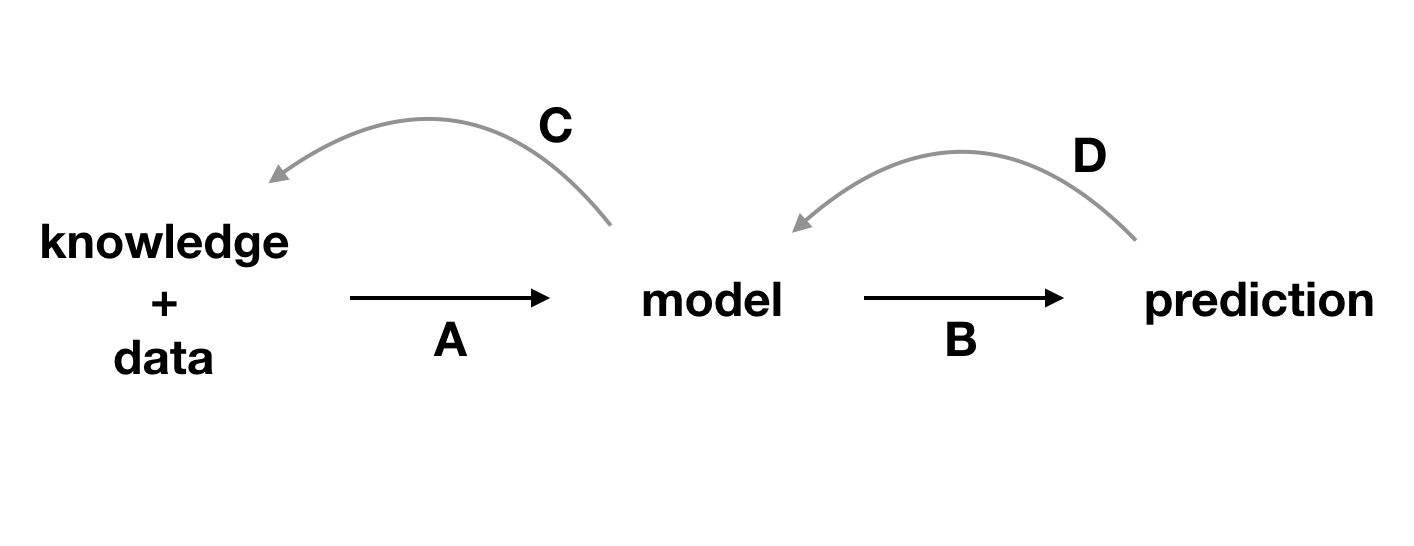
\includegraphics{figure/mp_understanding.png}
\caption{Workflow of a typical machine learning modeling. A) Modeling is
a process in which domain knowledge and data are turned into models. B)
Models are used to generate predictions. C) Understanding of a model
structure may increase our knowledge, and in consequence it may lead to
a better model. DALEX helps here. D) Understanding of drivers behind a
particular model's predictions may help to correct wrong decisions, and
in consequence it leads to a better model. DALEX helps here.}
\end{figure}

Variable importance

Model response as a function of a variable

Model performance / diagnostic / validation

\hypertarget{why-do-we-need-model-explainers}{%
\section{Why do we need model
explainers?}\label{why-do-we-need-model-explainers}}

Developer perspective:

AutoML

Feature Extraction

Model Improvement

Complex mthods are not being adopted quickly because people do not
understand them. Model explainers can change this and open new
applications

User perspective:

Justification of model decisions - civic rights

Model debudding / auditing

\citep{ONeil}

Cathy O'Neil: The era of blind faith in big data must end

``You don't see a lot of skepticism,'' she says. ``The algorithms are
like shiny new toys that we can't resist using. We trust them so much
that we project meaning on to them.'' Ultimately algorithms, according
to O'Neil, reinforce discrimination and widen inequality, ``using
people's fear and trust of mathematics to prevent them from asking
questions''.

But as Cathy O'Neil reveals in this urgent and necessary book, the
opposite is true. The models being used today are opaque, unregulated,
and uncontestable, even when they're wrong. Most troubling, they
reinforce discrimination: If a poor student can't get a loan because a
lending model deems him too risky (by virtue of his zip code), he's then
cut off from the kind of education that could pull him out of poverty,
and a vicious spiral ensues. Models are propping up the lucky and
punishing the downtrodden, creating a ``toxic cocktail for democracy.''
Welcome to the dark side of Big Data.

Bias w modelach:

\citep{2017arXiv171107076L}

Models may be biased. Examples for \citep{2017arXiv171006169T}

We propose a method to audit black-box risk models for potential bias by
using model distillation. We demonstrate the methods on four public
datasets: COMPAS, Lending Club, Stop-and-Frisk, and Chicago Police

\hypertarget{how-model-exploration-is-different-from-data-exploration}{%
\section{How model exploration is different from data
exploration?}\label{how-model-exploration-is-different-from-data-exploration}}

Similarities:

\begin{itemize}
\tightlist
\item
  Models and data are related to some truth that we want to understand
\item
  We use visuals to quicker understand complex relations
\end{itemize}

Differences:

\begin{itemize}
\tightlist
\item
  Data comes from some population; we treat them as a random sample. And
  since there is a sample there is also some randomness
\item
  Models are just functions. Most models are not stochastic and we
  consider only deterministic models.
\item
  We believe that data is noisy, but there is truth there. Data cannot
  be bad of misfitted, may be biased. Models can be bad, misfitted,
  unaccurate
\end{itemize}

\hypertarget{black-box-models-vs-white-box-models}{%
\section{Black-box models vs White-box
models}\label{black-box-models-vs-white-box-models}}

\citep{R-DALEX}

\hypertarget{model-agnostic-vs-model-specific}{%
\section{Model agnostic vs Model
specific}\label{model-agnostic-vs-model-specific}}

Tools designed to deal with specific models

\begin{itemize}
\tightlist
\item
  \citep{R-randomForestExplainer}
\item
  \citep{R-xgboostExplainer}
\item
  Specific for neural networks
\end{itemize}

Model agnostic

\begin{itemize}
\tightlist
\item
  DALEX, lime and all other presented in this book
\end{itemize}

\begin{Shaded}
\begin{Highlighting}[]
\KeywordTok{library}\NormalTok{(}\StringTok{"xgboostExplainer"}\NormalTok{)}
\end{Highlighting}
\end{Shaded}

\hypertarget{glossary-notation}{%
\section{Glossary / Notation}\label{glossary-notation}}

model healthcheck

Let \(f_{M}(x): \mathcal R^{d} \rightarrow \mathcal R\) denote a
predictive model, i.e.~function that takes \(d\) dimensional vector and
calculate numerical score. In section in which we work with larger
number of models we use subscript \(M\) to index models. But to simplify
notation, this subscript is omitted if profiles for only one model are
considered.

Symbol \(x \in \mathcal R^d\) refers to a point in the feature space. We
use subscript \(x_i\) to refer to a different data points and
superscript \(x^j\) to refer to specific dimensions. Additionally, let
\(x^{-j}\) denote all coordinates except \(j\)-th and let \(x|^j=z\)
denote a data point \(x^*\) with all coordinates equal to \(x\) except
coordinate \(j\) equal to value \(z\). I.e.
\(\forall_{i \neq {j}} x^i = x^{*,i}\) and \(x^j = z\). In other words
\(x|^j=z\) denote a \(x\) with \(j\)th coordinate changed to \(z\).

Now we can define Ceteris Paribus Profile for model \(f\), variable
\(j\) and point \(x\) as

\[
CP^{f, j, x}(z) := f(x|^j = z).
\] I.e. CP profile is a model response obtained for observations created
based on \(x\) with \(j\) coordinated changes and all other coordinates
kept unchanged.

It is convenient to use an alternative name for this plot: What-If
Plots. CP profiles show what would happen if only a single variable is
changed.

Figure 5.1 shows an example of Ceteris Paribus profile. The black dot
stands for prediction for a single observation. Grey line show how the
model response would change if in this single observation coordinate
\texttt{surface} will be changes to selected value. From this profile
one may read that the model response is non monotonic. If
\texttt{construction.year} for this observation would be below 1935 the
model response would be higher, but if construction year were between
1935 and 1995 the model response would be lower.

Glossary:

\begin{itemize}
\tightlist
\item
  Black-box model
\item
  White-box model
\item
  Feature
\item
  Variable
\item
  Continuous variable
\item
  Nominal variable
\item
  Model-agnostic / Model specific
\end{itemize}

\hypertarget{thanksto}{%
\section{Thanks to}\label{thanksto}}

We are using the \textbf{bookdown} package \citep{R-bookdown} in this
sample book

Chris Drake and Janusz Holyst

\hypertarget{prediction-level-explanations}{%
\chapter*{Prediction level
explanations}\label{prediction-level-explanations}}
\addcontentsline{toc}{chapter}{Prediction level explanations}

\hypertarget{PredictionExplainers}{%
\chapter{Introduction}\label{PredictionExplainers}}

Prediction level explainers help to understand how the model works for a
single prediction. This is the main difference from the model level
explainers that were focused on the model in general. Prediction level
explainers are always in context of a single observation.

Think about following use-cases

\begin{itemize}
\tightlist
\item
  One wants to attribute effects of variables to a model predictions.
  Think about model for hart attack. Having a final score for a patient
  one wants to understand how much of this score come from smoking or
  age or gender.
\item
  One wants to understand how the model response would change if some
  inputs are changed. Think about model for hart attack. How the model
  response would change if a patient cuts the number of smoked
  cigarettes by half.
\item
  Model is not working correctly for a particular point and one wants to
  understand why predictions for this point are wrong.
\end{itemize}

\hypertarget{variable-attribution-vs-what-if-analysis}{%
\section{Variable attribution vs What-if
analysis}\label{variable-attribution-vs-what-if-analysis}}

TODO: varaible attribution is not sparse, no reason for them to be like
that

TODO: Three approaches: variable attribution, local model,

TODO: condvis \citep{JSSv081i05}

Enslaving the Algorithm: From a `Right to an Explanation' to a `Right to
Better Decisions'? \citep{Edwards_Veale_2018}

TODO: Sparse model approximation / variable selection / feature ranking

There are many different tools that may be used to explore model around
a single data point and in following sections we will describe the most
popular approaches. They can be divided into two classes.

\begin{itemize}
\tightlist
\item
  Analysis of the model curvature. Here we treat the model as a function
  and we are interested in the curvature of this function around the
  point of interest (see Figure \ref{fig:modelResponseCurve}). In the
  Section \ref{LIME} we present the LIME method that approximates the
  black-box model in a point of interest while in section
  \ref{ceterisParibus} we present Ceteris Paribus profiles that are more
  focused on conditional changes of model response given only one
  coordinate is modified.
\item
  Analysis of the probabilistic behavior of the model. Here we are
  interested in decomposition of the model response to parts that can be
  attributed to particular features.
\end{itemize}

\begin{figure}
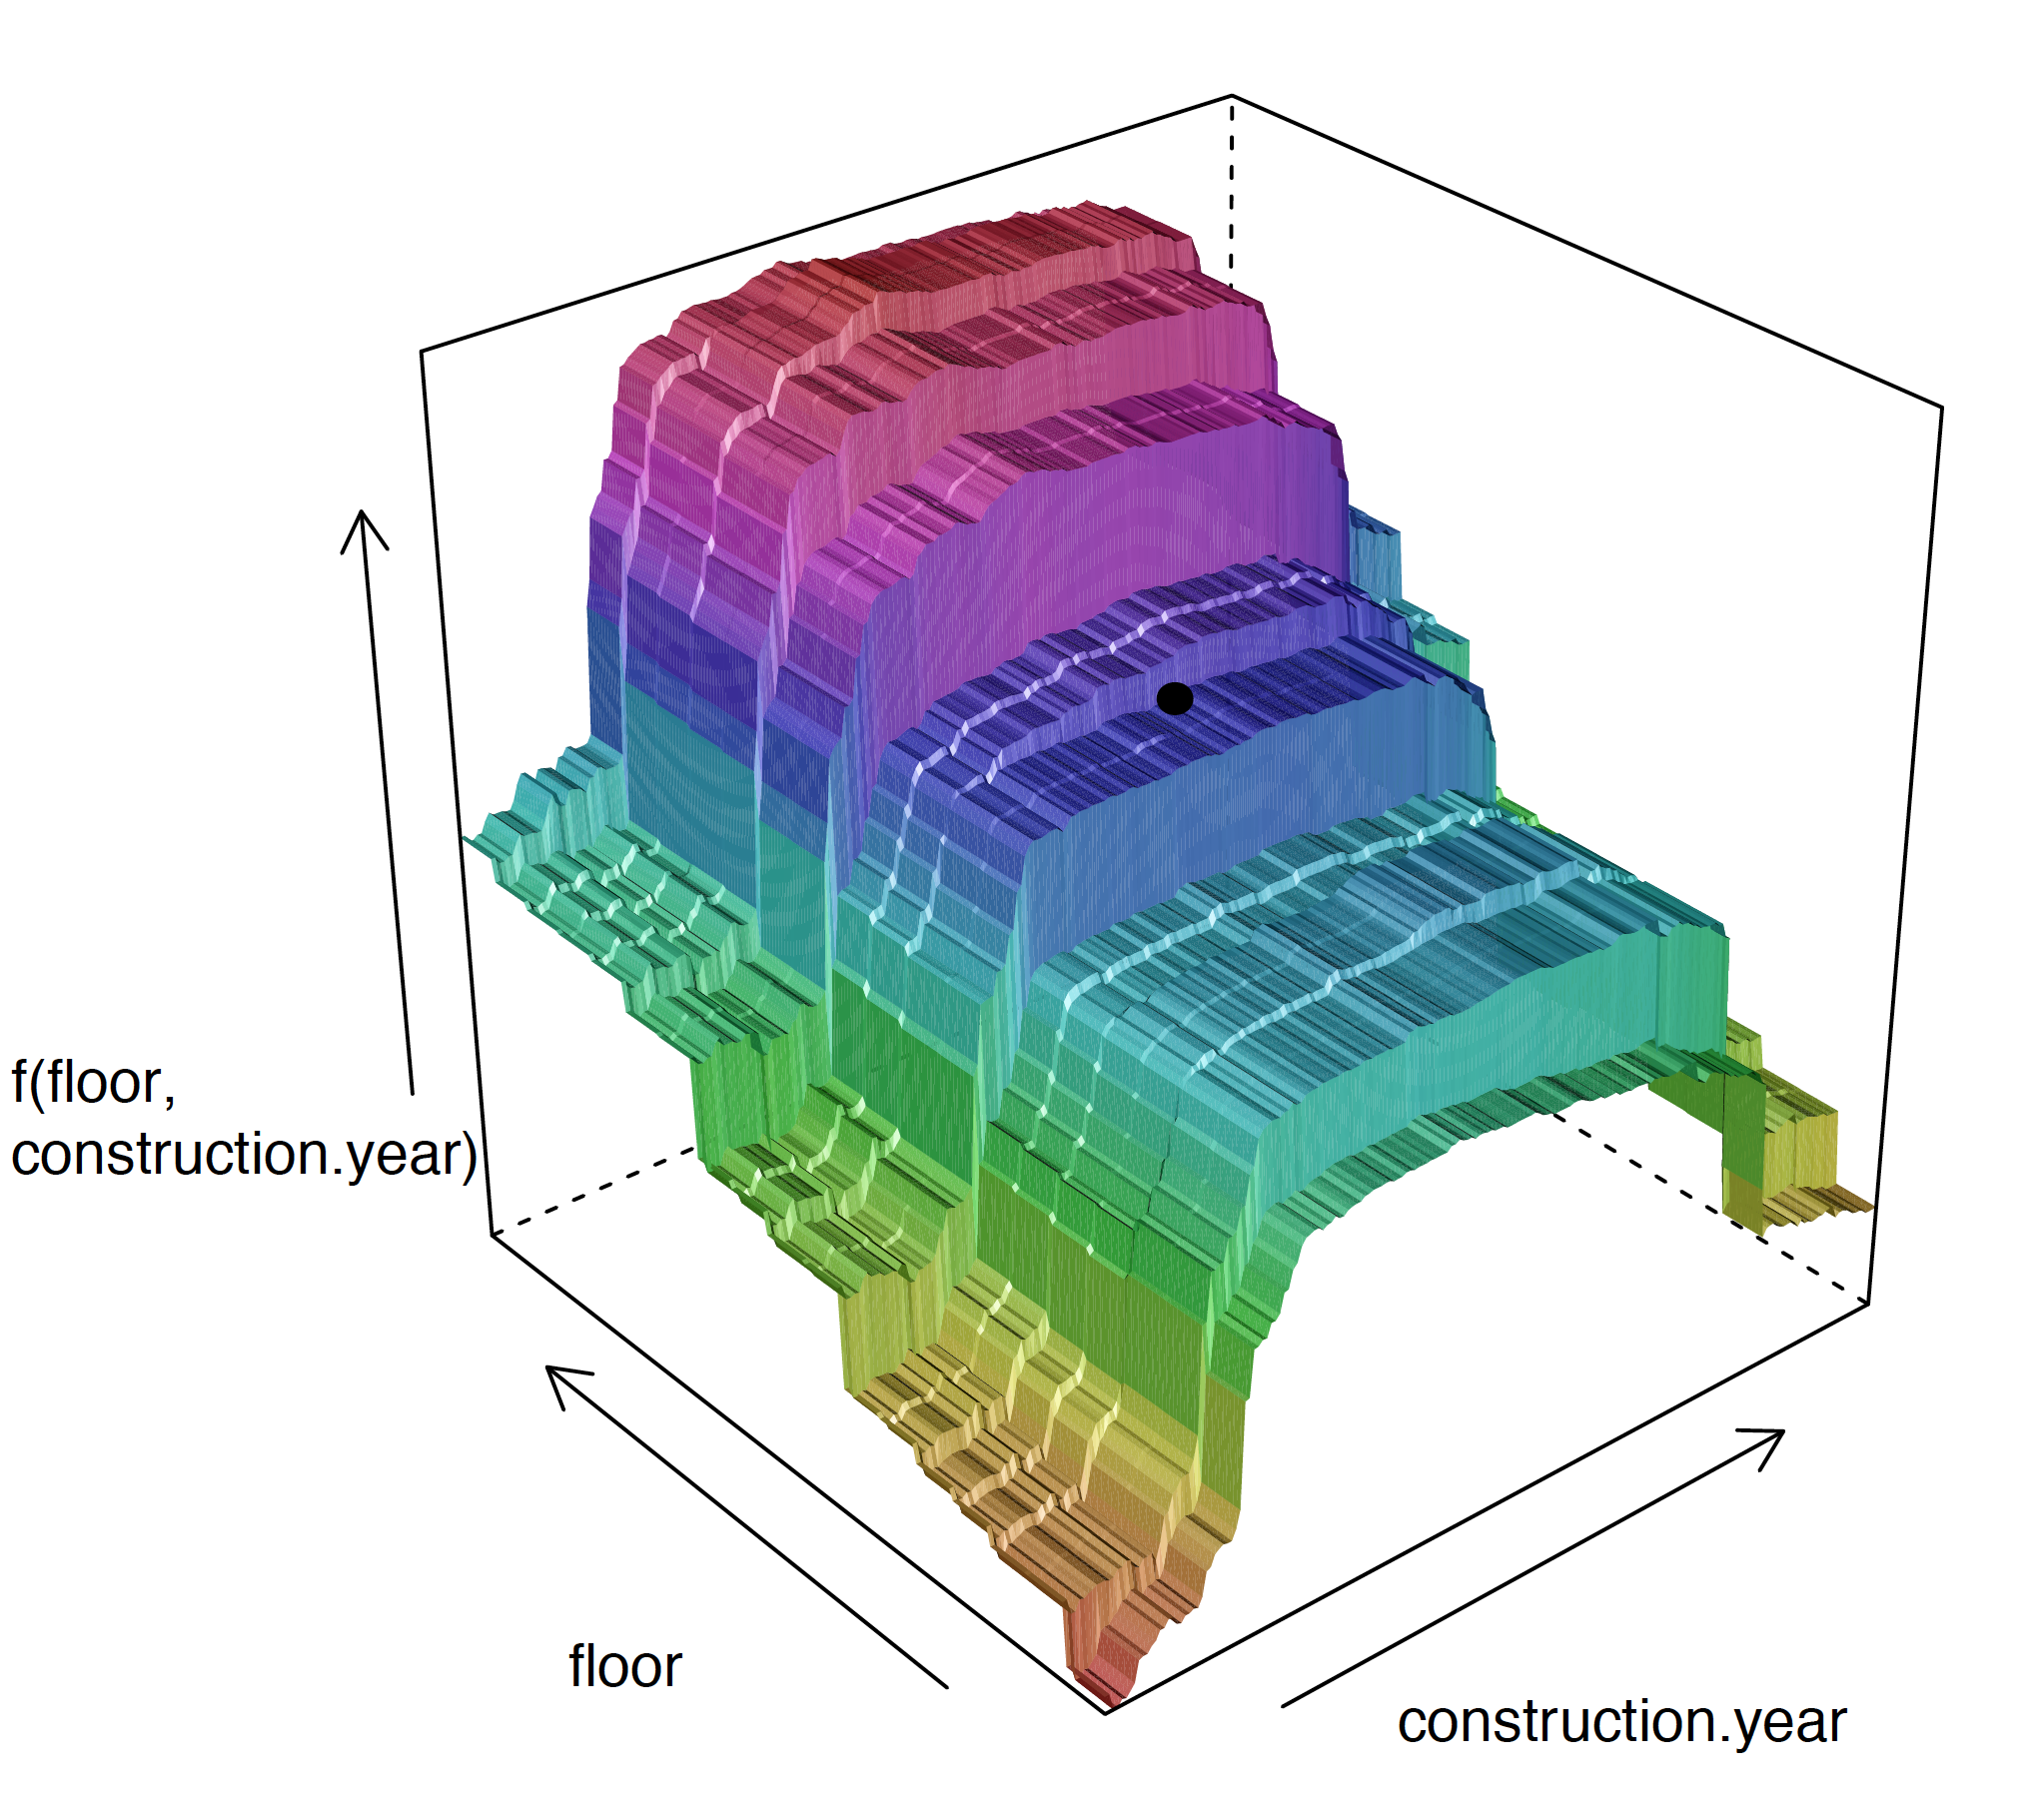
\includegraphics[width=0.7\linewidth]{figure/model_response} \caption{(fig:modelResponseCurve) Model response surface. We are interested in understanding the model behavior in a single point}\label{fig:modelResponseCurve}
\end{figure}

\hypertarget{when-to-use}{%
\section{When to use?}\label{when-to-use}}

There are several use-cases for such explainers. Think about following.

\begin{itemize}
\tightlist
\item
  Model improvement. If model works particular bad for a selected
  observation (the residual is very high) then investigation of model
  responses for miss fitted points may give some hints how to improve
  the model. For individual predictions it is easier to notice that
  selected variable should have different a effect.
\item
  Additional domain specific validation. Understanding which factors are
  important for model predictions helps to be critical about model
  response. If model contributions are against domain knowledge then we
  may be more skeptical and willing to try another model. On the other
  hand, if the model response is aligned with domain knowledge we may
  trust more in these responses. Such trust is important in decisions
  that may lead to serious consequences like predictive models in
  medicine.
\item
  Model selection. Having multiple candidate models one may select the
  final response based on model explanations. Even if one model is
  better in terms of global model performance it may happen that locally
  other model is better fitted. This moves us towards model
  consultations that identify different options and allow human to
  select one of them.
\end{itemize}

\hypertarget{three-single-laws}{%
\section{A bit of philosophy: Three Laws for Prediction Level
Explanations}\label{three-single-laws}}

76 years ago Isaac Asimov devised
\href{https://en.wikipedia.org/wiki/Three_Laws_of_Robotics}{Three Laws
of Robotics}: 1) a robot may not injure a human being, 2) a robot must
obey the orders given it by human beings and 3) A robot must protect its
own existence. These laws impact discussion around
\href{https://en.wikipedia.org/wiki/Ethics_of_artificial_intelligence}{Ethics
of AI}. Today's robots, like cleaning robots, robotic pets or autonomous
cars are far from being conscious enough to be under Asimov's ethics.

Today we are surrounded by complex predictive algorithms used for
decision making. Machine learning models are used in health care,
politics, education, judiciary and many other areas. Black box
predictive models have far larger influence on our lives than physical
robots. Yet, applications of such models are left unregulated despite
many examples of their potential harmfulness. See \emph{Weapons of Math
Destruction} by Cathy O'Neil for an excellent overview of potential
problems.

It's clear that we need to control algorithms that may affect us. Such
control is in our civic rights. Here we propose three requirements that
any predictive model should fulfill.

\begin{itemize}
\tightlist
\item
  \textbf{Prediction's justifications}. For every prediction of a model
  one should be able to understand which variables affect the prediction
  and how strongly. Variable attribution to final prediction.
\item
  \textbf{Prediction's speculations}. For every prediction of a model
  one should be able to understand how the model prediction would change
  if input variables were changed. Hypothesizing about what-if
  scenarios.
\item
  \textbf{Prediction's validations} For every prediction of a model one
  should be able to verify how strong are evidences that confirm this
  particular prediction.
\end{itemize}

There are two ways to comply with these requirements. One is to use only
models that fulfill these conditions by design. White-box models like
linear regression or decision trees. In many cases the price for
transparency is lower performance. The other way is to use approximated
explainers -- techniques that find only approximated answers, but work
for any black box model. Here we present such techniques.

\hypertarget{introduction-to-variable-attribution-methods}{%
\chapter{Introduction to variable attribution
methods}\label{introduction-to-variable-attribution-methods}}

In this section we introduce method for additive decomposition of
predictions. The main goal for these tools is to help understand how
model output may be attributed to input variables or sets of variables.

Presented explainers are linked with the first law introduced in Section
\ref{three-single-laws}, i.e.~law for prediction's justifications. Note
that there are more tools for variable attribution, some of them will be
presented in next sections.

Think of following use cases:

\begin{itemize}
\tightlist
\item
  Think about a model for heart attack. A patient wants to know which
  factors have highest impact on the final heart risk score.
\item
  Think about a model for apartment prices. An investor wants to know
  how much of the final price may be attributed to the location of an
  apartment.
\item
  Think about a model for credit scoring. A customer wants to know if
  factors like gender, age or number of kids influence model decisions.
\end{itemize}

In the section \ref{VAlinMod} we will introduce key concepts and
intuitions beyond variable attribution based on linear models. This
approach may be easily applied to additive models and generalized linear
models. In sections \ref{breakDown} and \ref{shapley} we will present
model agnostic extentions of this concept.

\hypertarget{VAlinMod}{%
\section{Variable attribution for linear models}\label{VAlinMod}}

Linear model with coefficients
\(\beta = (\beta_0, \beta_1, .., \beta_p)\) has following form.

\[
f(x) = \beta_0 + x_1 \beta_1 + \ldots + x_p \beta_p.
\] In other words, model response is the sum of weighted elements of
\(x = (x_1, x_2, \ldots, x_p)\).

From a global perspective of a model, we are usually interested in
questions like, how good is the model, which variables are significant
or how accurate are model predictions.

But in this chapter we are focues in a local perspective, i.e.~for a
single observation \(x^*\) how to measure the contribution of a variable
\(x_i\) on model prediction \(f(x^*)\).

Let \(v(f, x^*, i)\) stands for the contribution of variable \(x_i\) on
prediction of model \(f()\) in point \(x^*\). For linear models it is
easy to define such contribution as \[
v(f, x^*, i) = f(x^*) - E[f(x)|x_{-1} = x^*_{-1}] = \beta_i x^*_i  - E \beta_i X_i
\] where the expected value can be estimated from the data \[
v(f, x^*, i) = \beta_i x^*_i - \beta_i \bar x_i = \beta_i (x^*_i - \bar x_i)
\]

The logic behind the attribution is the following. Contribution of
variable \(x_i\) is the difference between model response for value
\(x_i^*\) minus the average model response.

\hypertarget{wine-quality-example}{%
\subsection{Wine quality example}\label{wine-quality-example}}

It may be a surprise, that the attribution for variable \(x_i\) is not
the \(\beta_i x_i\). But, please consider following example. Figure
\ref{fig:attribution1} shows the relation between alcohol and wine
quality, based on the wine dataset \citep{wine2009}. The corresponding
linear model is

\[
quality(alcohol) = 2.5820 + 0.3135 * alcohol
\]

The weakest wine in this dataset has 8\% of alcohol, average alcohol
concentration is 10.51, so the contribution of alcohol to the model
prediction is \(0.3135 *(8-10.51) = -0.786885\). It means that low value
of alcohol for this wine (8\%) lower the prediction of quality by
\(-0.786885\).

Note, that it would be confusing to forget about normalisation and say,
that for the alcohol contribution on quality is \(0.3135*8 = 2.508\) as
this is high positive value.

\begin{figure}

{\centering 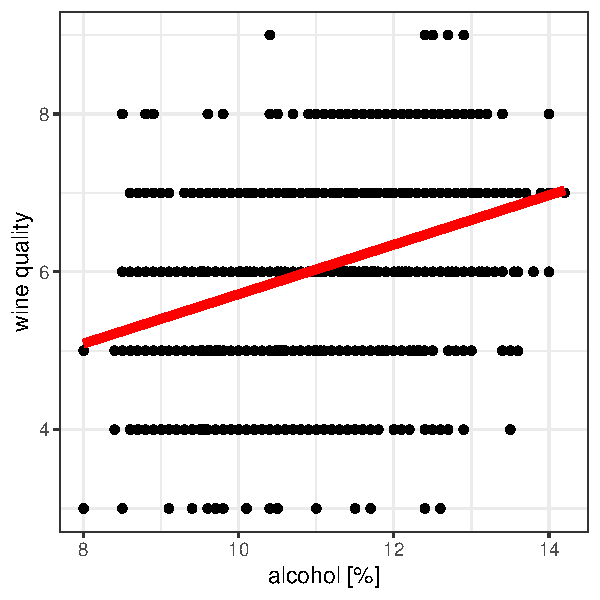
\includegraphics[width=0.5\linewidth]{figure/attribution_1} 

}

\caption{(fig:attribution1)Relation between wine quality and concentration of alcohol assessed with linear model}\label{fig:attribution1}
\end{figure}

Note that the linear model ma be rewritten in a following way

\[
f(x) = baseline + (x_1 - \bar x_1) \beta_1 + ... + (x_p - \bar x_p) \beta_p
\]

where \[
baseline = \mu + \bar x_1 \beta_1 + ... + \bar x_p \beta_p.
\]

Here \(baseline\) is an average model response and variable
contributions show how prediction for particular \(x^*\) is different
from the average response.

** NOTE for careful readers **

There is a gap between expected value of \(X_i\) and average calculated
on some dataset \(\bar x_i\). The latter depends on the data used for
calculation of averages. For the sake of simplicity we do not emphasise
these differences. To live with this just assume that we have access to
a very large validation data that allows us to calculate \(\bar x_i\)
very accurately.

\hypertarget{modelAgnosticAttribution}{%
\section{Model agnostic approaches}\label{modelAgnosticAttribution}}

In the Section \ref{VAlinMod} we introduced a method for calculation of
variable attributions for linear models. This method is accurate, based
directly on the structure of the model. But for most popular machine
learning models we cannot assume that they are linear nor even additive.

In next sections we introduce a model agnostic approach. Note that even
if the model itself is not additive, the model attribution will be
additive.

Again, let \(v(f, x^*, i)\) stands for the contribution of variable
\(x_i\) on prediction of model \(f()\) in point \(x^*\).

We expect that such contribution will sum up to the model prediction in
a given point (property called \emph{local accuracy}), so \[
f(x^*) = baseline + \sum_{i=1}^p v(f, x^*, i)
\] where \(baseline\) stands for average model response.

Note that the equation above may be rewritten as

\[
E [f(X)|X_1 = x_1^*, \ldots, X+p = x_p^*] = E[f(X)] + \sum_{i=1}^p v(f, x^*, i)
\] what leads to quite natural proposition for \(v(f, x^*_i, i)\), such
as

\[
v(f, x^*_i, i) = E [f(X) | X_1 = x_1^*, \ldots, X_i = x_i^*] - E [f(X) | X_1 = x_1^*, \ldots, X_{i-1} = x_{i-1}^*] 
\] In other words the contribution of variable \(i\) is the difference
between expected model response conditioned on first \(i\) variables
minus the model response conditioned on first \(i-1\) variables.

Such proposition fulfills the \emph{local accuracy} condition, but
unfortunatelly variable contributions depends on the ordering of
variables.

\begin{figure}

{\centering 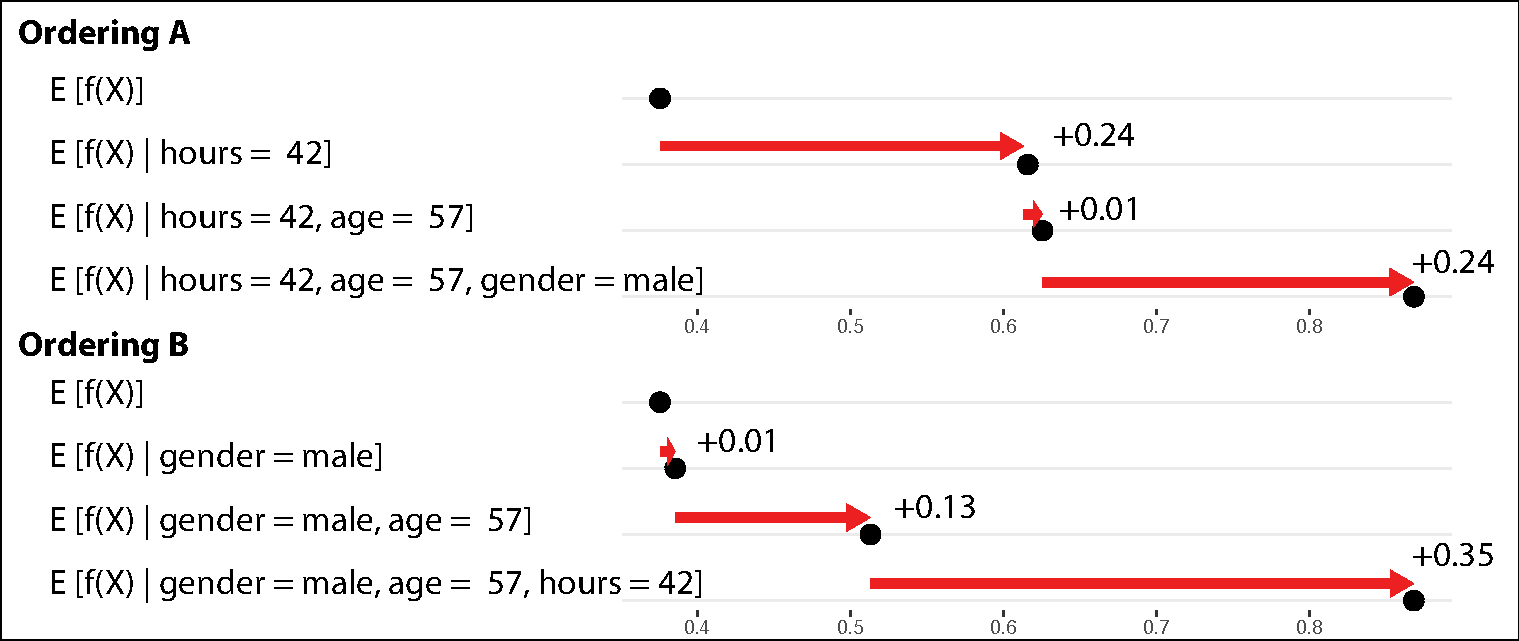
\includegraphics[width=1\linewidth]{figure/ordering} 

}

\caption{(fig:ordering) Two different paths between average model prediction and the model prediction for a selected observation. Black dots stand for conditional average, red arrows stands for changes between conditional averages.}\label{fig:ordering}
\end{figure}

See for example Figure \ref{fig:ordering}. In the first ordering the
contribution of variable \texttt{age} is calculated as 0.01, while in
the second the contribution is calculated as 0.13. Such differences are
related to the lack of additivness of the model \(f()\). Propositions
presented in next two sections present different solutions for this
problem.

\hypertarget{breakDown}{%
\chapter{Break Down Attributions}\label{breakDown}}

The approach for variable attribution presented in the Section
\ref{modelAgnosticAttribution} has the property of \emph{local
accuracy}, but variable contributions depends on the variable ordering.

The Break Down method solves this problem by using two-step procedure.
In the first step variables are ordered and in the second step the
consecutive conditioning is applied to ordered variables.

\hypertarget{the-algorithm}{%
\section{The Algorithm}\label{the-algorithm}}

First step of this algorithm is to determine the order of variables for
conditioning. It seems to be reasonable to include first variables that
are likely to be most important, leaving the noise variables at the end.
This leads to order based on following scores

\[
score(f, x^*, i) = \left| E [f(X)] - E [f(X)|X_i = x^*_i] \right|
\] Note, that the absolute value is needed as variable contributions can
be both positive and negative.

Once the ordering is determined in the second step variable
contributions are calculated as

\[
v(f, x^*_i, i) = E [f(X) | X_{I \cup \{i\}} = x_{I \cup \{i\}}^*] - E [f(X) | X_{I} = x_{I}^*] 
\] where \(I\) is the set of variables that have scores smaller than
score for variable \(i\).

\[
I = \{j: score(f, x^*, j) < score(f, x^*, i)\}
\]

The time complexity of the first step id \(O(p)\) where \(p\) is the
number of variables and the time complexity of the second step is also
\(O(p)\).

\hypertarget{hr-dataset-hire-or-fire}{%
\section{HR dataset: Hire or Fire?}\label{hr-dataset-hire-or-fire}}

Let us consider a random forest model created for HR data. The average
model response is \(\bar f(x) = 0.385586\). For a selected observation
\(x^*\) the table below presents scores for particular variables.

\begin{longtable}[]{@{}lrr@{}}
\toprule
& Ei f(X) & scorei\tabularnewline
\midrule
\endhead
hours & 0.616200 & 0.230614\tabularnewline
salary & 0.225528 & 0.160058\tabularnewline
evaluation & 0.430994 & 0.045408\tabularnewline
age & 0.364258 & 0.021328\tabularnewline
gender & 0.391060 & 0.005474\tabularnewline
\bottomrule
\end{longtable}

Once we determine the order we can calculate sequential contributions

\begin{longtable}[]{@{}lrr@{}}
\toprule
variable & cumulative & contribution\tabularnewline
\midrule
\endhead
(Intercept) & 0.385586 & 0.385586\tabularnewline
* hours = 42 & 0.616200 & 0.230614\tabularnewline
* salary = 2 & 0.400206 & -0.215994\tabularnewline
* evaluation = 2 & 0.405776 & 0.005570\tabularnewline
* age = 58 & 0.497314 & 0.091538\tabularnewline
* gender = male & 0.778000 & 0.280686\tabularnewline
final\_prognosis & 0.778000 & 0.778000\tabularnewline
\bottomrule
\end{longtable}

\hypertarget{break-down-plots}{%
\section{Break Down Plots}\label{break-down-plots}}

Once we calculated variable attributions we may plot them in an
intuitive form. This intuition behind Break Down Plots is described in
Figure \ref{BDPrice4}.

The variable ordering determined in the first step of Break Down
Algorithm is reflected by the ordering of variables in rows of the plot.

The last row of a plot shows the \(baseline\), i.e.~an average model
prediction. The next row corresponds to average model prediction for
observations with variable \texttt{surface} fixed to value \texttt{35}.
The next for corresponds to average model prediction with variables
\texttt{surface} set to \texttt{35} and \texttt{floor} set to
\texttt{1}, and so on. The first row corresponds to model response for
\(x^*\).

In panels A and B violines show distribution of model predictions for
selected points, while red dots stands for averages.

The most minimal form that shows important information is presented in
the panel C. Positive values are presented with green bars while
negative differences are marked with yellow bar. They sum up to final
model prediction, which is denoted by a grey bar in this example.

\begin{figure}

{\centering 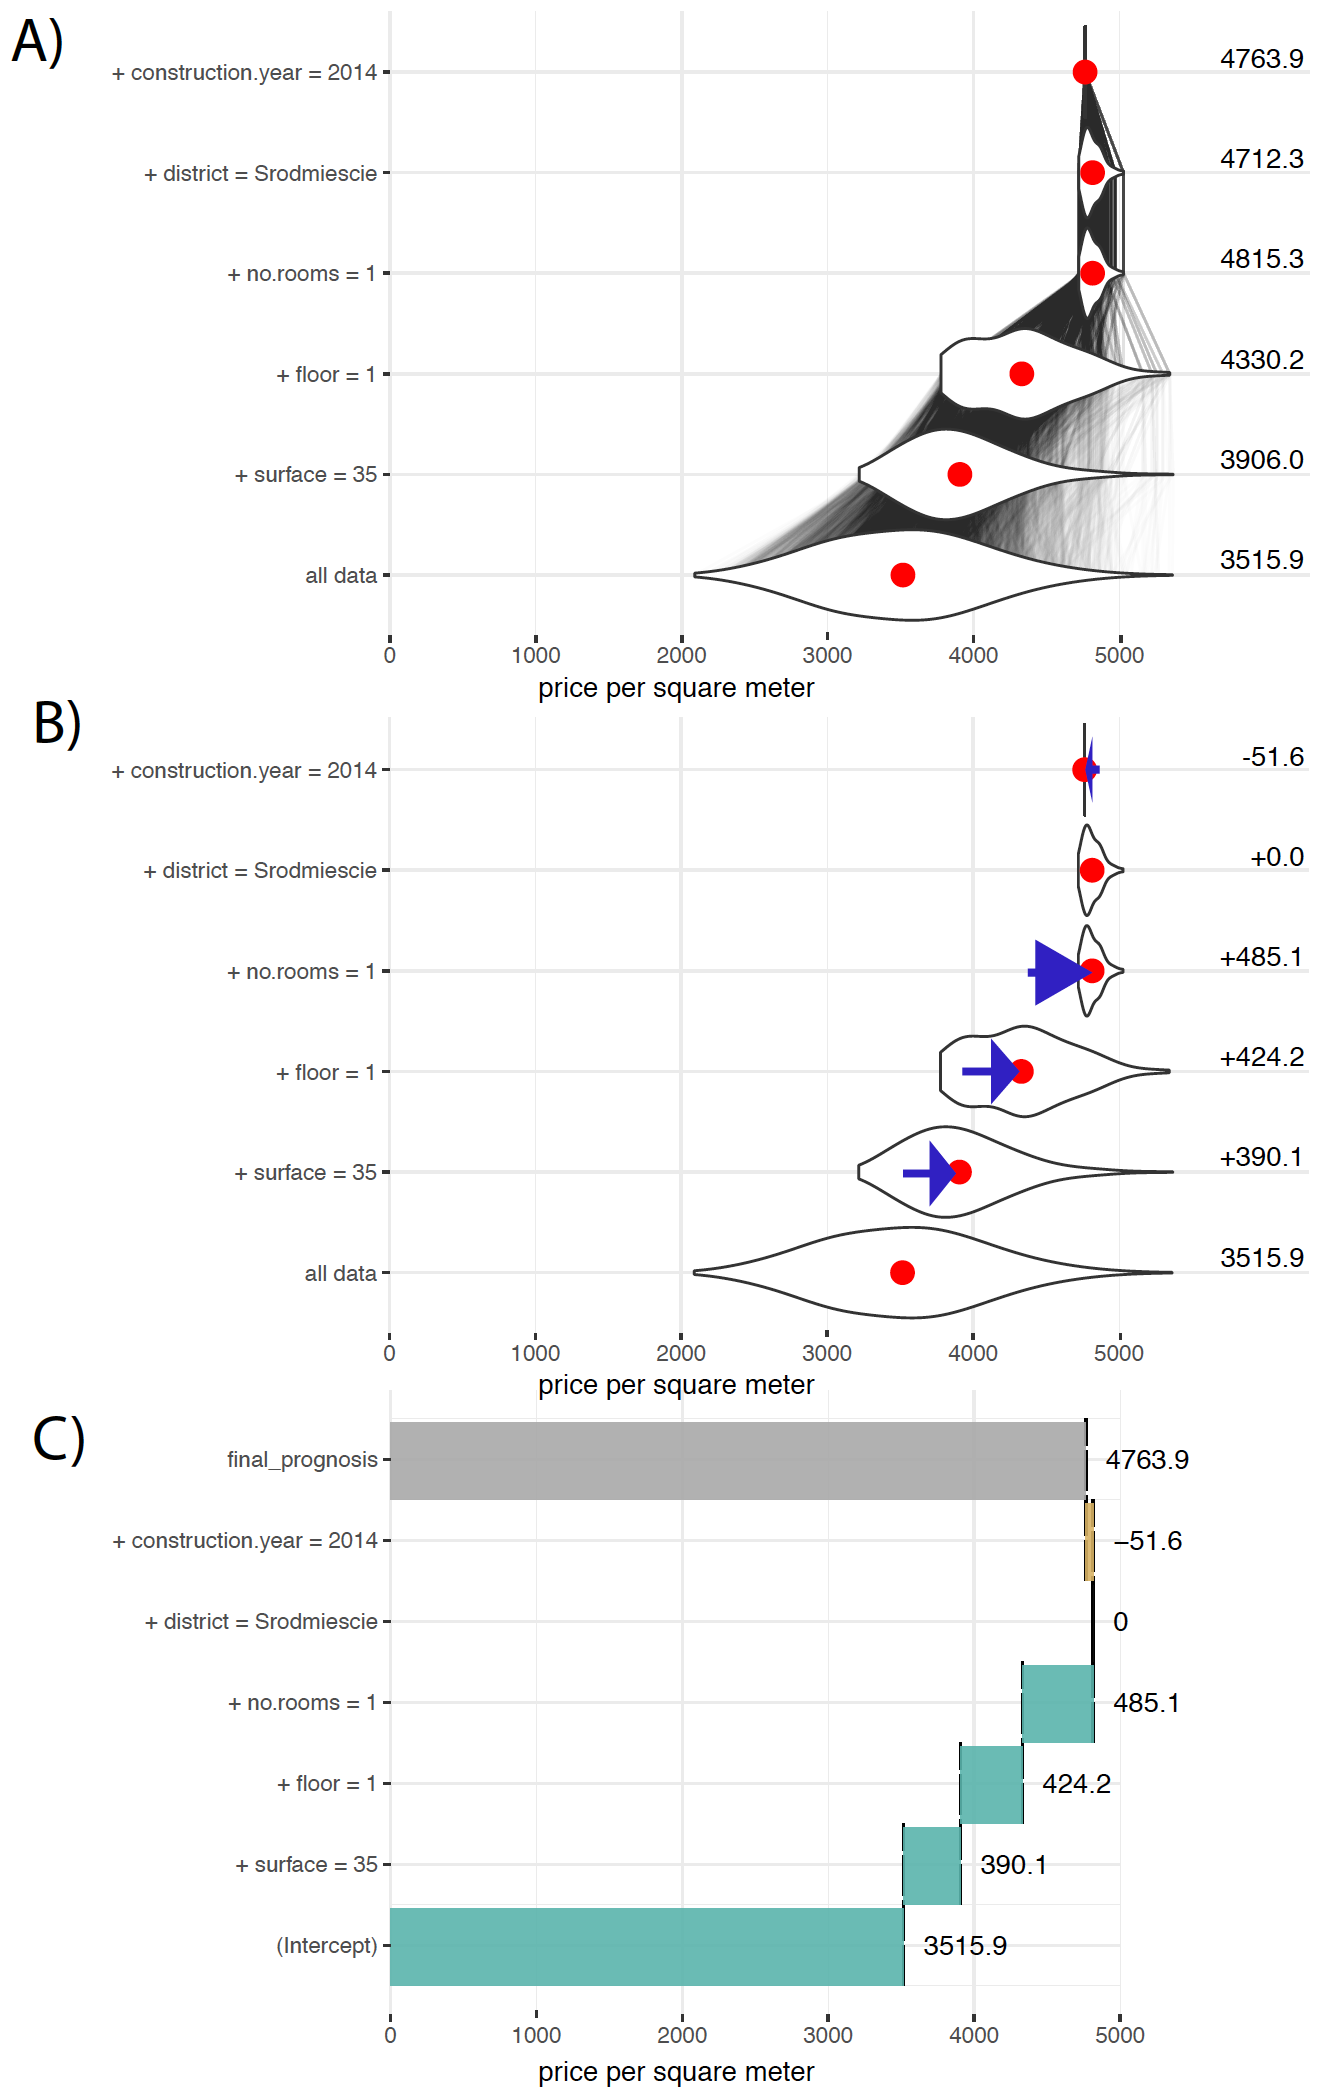
\includegraphics[width=0.7\linewidth]{figure/bd_price_4} 

}

\caption{(fig:BDPrice4) Break Down Plots show how variables move the model prediction from population average to the model prognosis for a single observation. A) The last row shows distribution of model predictions. Next rows show conditional distributions, every row a new variable is added to conditioning. The first row shows model prediction for a single point. Red dots stand for averages. B) Blue arrows shows how the average conditional response change, these values are variables contributions. C) Only variable contributions are presented. }\label{fig:BDPrice4}
\end{figure}

\hypertarget{pros-and-cons}{%
\section{Pros and cons}\label{pros-and-cons}}

Break Down approach is model agnostic, can be applied to any predictive
model that returns a single number. It leads to additive variable
attribution. Below we summarize key strengths and weaknesses of this
approach.

\textbf{Pros}

\begin{itemize}
\tightlist
\item
  Break Down Plots are easy to understand and decipher.
\item
  Break Down Plots are compact; many variables may be presented in a
  small space.
\item
  Break Down Plots are model agnostic yet they reduce to intuitive
  interpretation for linear Gaussian and generalized models.
\item
  Complexity of Break Down Algorithm is linear in respect to the number
  of variables.
\end{itemize}

\textbf{Cons}

\begin{itemize}
\tightlist
\item
  If the model is non-additive then showing only additive contributions
  may be misleading.
\item
  Selection of the ordering based on scores is subjective. Different
  orderings may lead to different contributions.
\item
  For large number of variables the Break Down Plot may be messy with
  many variables having small contributions.
\end{itemize}

\hypertarget{code-snippets-for-r}{%
\section{Code snippets for R}\label{code-snippets-for-r}}

In this section we present key features of the \texttt{breakDown}
package for R \citep{R-breakDown}. This package covers all features
presented in this chapter. It is available on CRAN and GitHub. Find more
examples at the website of this package
\texttt{https://pbiecek.github.io/breakDown/}.

\textbf{Model preparation}

In this section we will present an example based on the \texttt{HR}
dataset and Random Forest model \citep{R-randomForest}. See the Section
\ref{HRdataset} for more details.

\begin{Shaded}
\begin{Highlighting}[]
\KeywordTok{library}\NormalTok{(}\StringTok{"DALEX"}\NormalTok{)}
\KeywordTok{library}\NormalTok{(}\StringTok{"randomForest"}\NormalTok{)}
\NormalTok{model <-}\StringTok{ }\KeywordTok{randomForest}\NormalTok{(status }\OperatorTok{~}\StringTok{ }\NormalTok{gender }\OperatorTok{+}\StringTok{ }\NormalTok{age }\OperatorTok{+}\StringTok{ }\NormalTok{hours }\OperatorTok{+}\StringTok{ }\NormalTok{evaluation }\OperatorTok{+}\StringTok{ }\NormalTok{salary, }\DataTypeTok{data =}\NormalTok{ HR)}
\NormalTok{model}
\end{Highlighting}
\end{Shaded}

\begin{verbatim}
## 
## Call:
##  randomForest(formula = status ~ gender + age + hours + evaluation +      salary, data = HR) 
##                Type of random forest: classification
##                      Number of trees: 500
## No. of variables tried at each split: 2
## 
##         OOB estimate of  error rate: 27.23%
## Confusion matrix:
##          fired   ok promoted class.error
## fired     2272  394      189   0.2042032
## ok         523 1259      439   0.4331382
## promoted   201  391     2179   0.2136413
\end{verbatim}

Model exploration with the \texttt{breakDown} package is performed in
three steps.

\textbf{1. Create an explainer - wrapper around model and validation
data.}

Since all other functions work in a model agnostic fashion, first we
need to define a wrapper around the model. Here we are using the
\texttt{explain()} function from \texttt{DALEX} package \citep{R-DALEX}.

\begin{Shaded}
\begin{Highlighting}[]
\NormalTok{explainer_rf_fired <-}\StringTok{ }\KeywordTok{explain}\NormalTok{(model,}
                 \DataTypeTok{data =}\NormalTok{ HR,}
                 \DataTypeTok{y =}\NormalTok{ HR}\OperatorTok{$}\NormalTok{status }\OperatorTok{==}\StringTok{ "fired"}\NormalTok{,}
                 \DataTypeTok{predict_function =} \ControlFlowTok{function}\NormalTok{(m,x) }\KeywordTok{predict}\NormalTok{(m,x, }\DataTypeTok{type =} \StringTok{"prob"}\NormalTok{)[,}\DecValTok{1}\NormalTok{],}
                 \DataTypeTok{label =} \StringTok{"fired"}\NormalTok{)}
\end{Highlighting}
\end{Shaded}

\textbf{2. Select an observation of interest.}

Break Down Plots decompose model prediction around a single observation.
Let's construct a data frame with corresponding values.

\begin{Shaded}
\begin{Highlighting}[]
\NormalTok{new_observation <-}\StringTok{ }\KeywordTok{data.frame}\NormalTok{(}\DataTypeTok{gender =} \KeywordTok{factor}\NormalTok{(}\StringTok{"male"}\NormalTok{, }\DataTypeTok{levels =} \KeywordTok{c}\NormalTok{(}\StringTok{"male"}\NormalTok{, }\StringTok{"female"}\NormalTok{)),}
                      \DataTypeTok{age =} \FloatTok{57.7}\NormalTok{,}
                      \DataTypeTok{hours =} \FloatTok{42.3}\NormalTok{,}
                      \DataTypeTok{evaluation =} \DecValTok{2}\NormalTok{,}
                      \DataTypeTok{salary =} \DecValTok{2}\NormalTok{)}

\KeywordTok{predict}\NormalTok{(model, new_observation, }\DataTypeTok{type =} \StringTok{"prob"}\NormalTok{)}
\end{Highlighting}
\end{Shaded}

\begin{verbatim}
##   fired    ok promoted
## 1  0.79 0.202    0.008
## attr(,"class")
## [1] "matrix" "votes"
\end{verbatim}

\textbf{3. Calculate Break Down decomposition}

The \texttt{break\_down()} function calculates Break Down contributions
for a selected model around a selected observation.

The result from \texttt{break\_down()} function is a data frame with
variable attributions.

\begin{Shaded}
\begin{Highlighting}[]
\KeywordTok{library}\NormalTok{(}\StringTok{"breakDown"}\NormalTok{)}
\NormalTok{bd_rf <-}\StringTok{ }\KeywordTok{break_down}\NormalTok{(explainer_rf_fired,}
\NormalTok{                 new_observation,}
                 \DataTypeTok{check_interactions =} \OtherTok{FALSE}\NormalTok{,}
                 \DataTypeTok{keep_distributions =} \OtherTok{TRUE}\NormalTok{)}

\NormalTok{bd_rf}
\end{Highlighting}
\end{Shaded}

\begin{verbatim}
##                  contribution
## (Intercept)             0.375
## * hours = 42            0.239
## * salary = 2           -0.206
## * evaluation = 2        0.015
## * age = 58              0.069
## * gender = male         0.298
## final_prognosis         0.790
## baseline:  0
\end{verbatim}

The generic \texttt{plot()} function creates a Break Down plots.

\begin{Shaded}
\begin{Highlighting}[]
\KeywordTok{plot}\NormalTok{(bd_rf) }
\end{Highlighting}
\end{Shaded}

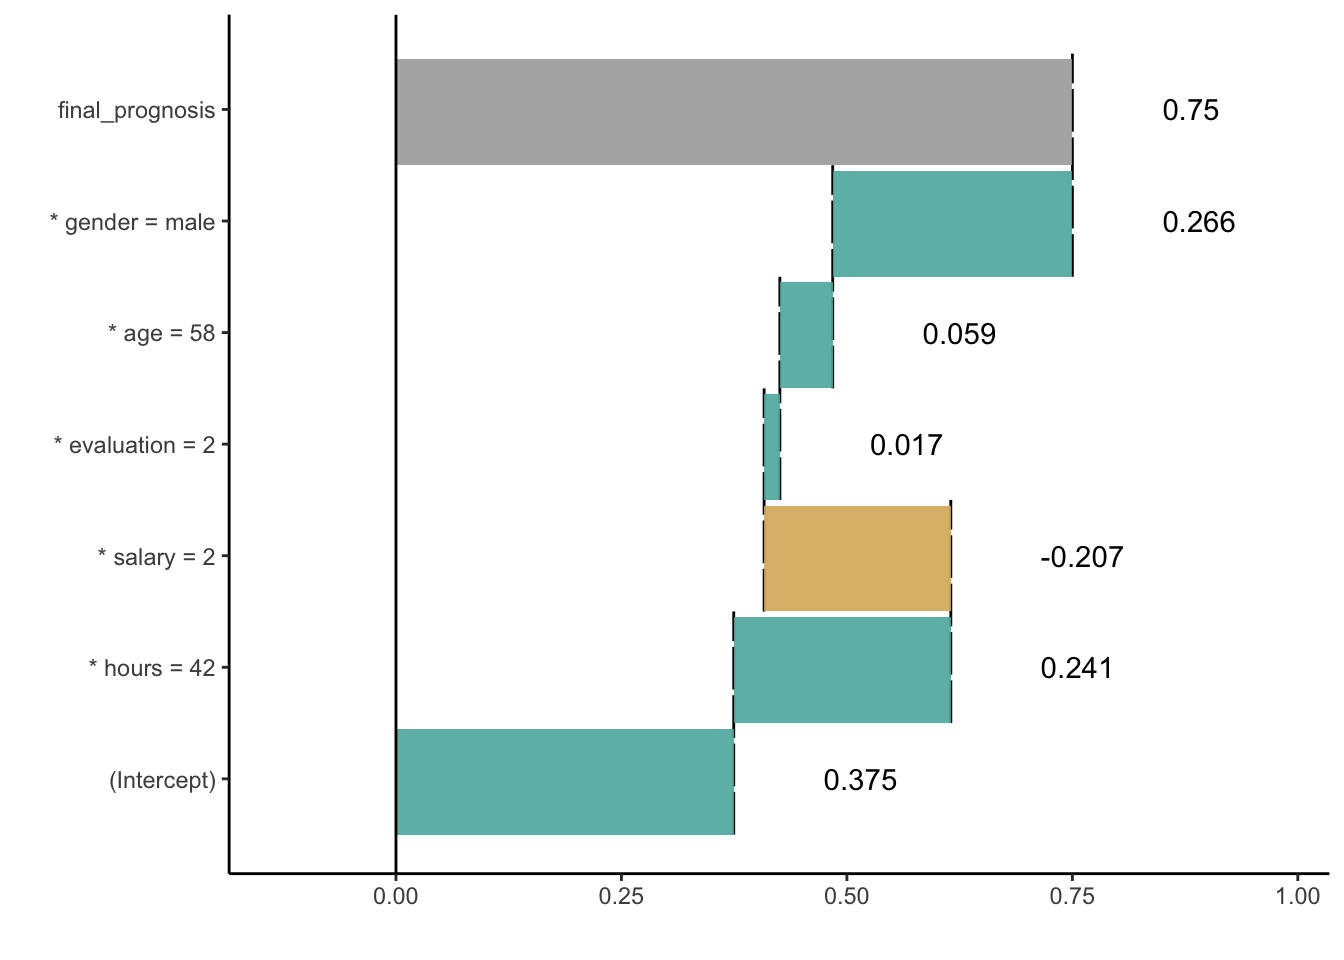
\includegraphics{PM_VEE_files/figure-latex/unnamed-chunk-8-1.pdf}

Add the \texttt{plot\_distributions\ =\ TRUE} argument to enrich model
response with additional information.

\begin{Shaded}
\begin{Highlighting}[]
\KeywordTok{plot}\NormalTok{(bd_rf, }\DataTypeTok{plot_distributions =} \OtherTok{TRUE}\NormalTok{) }
\end{Highlighting}
\end{Shaded}

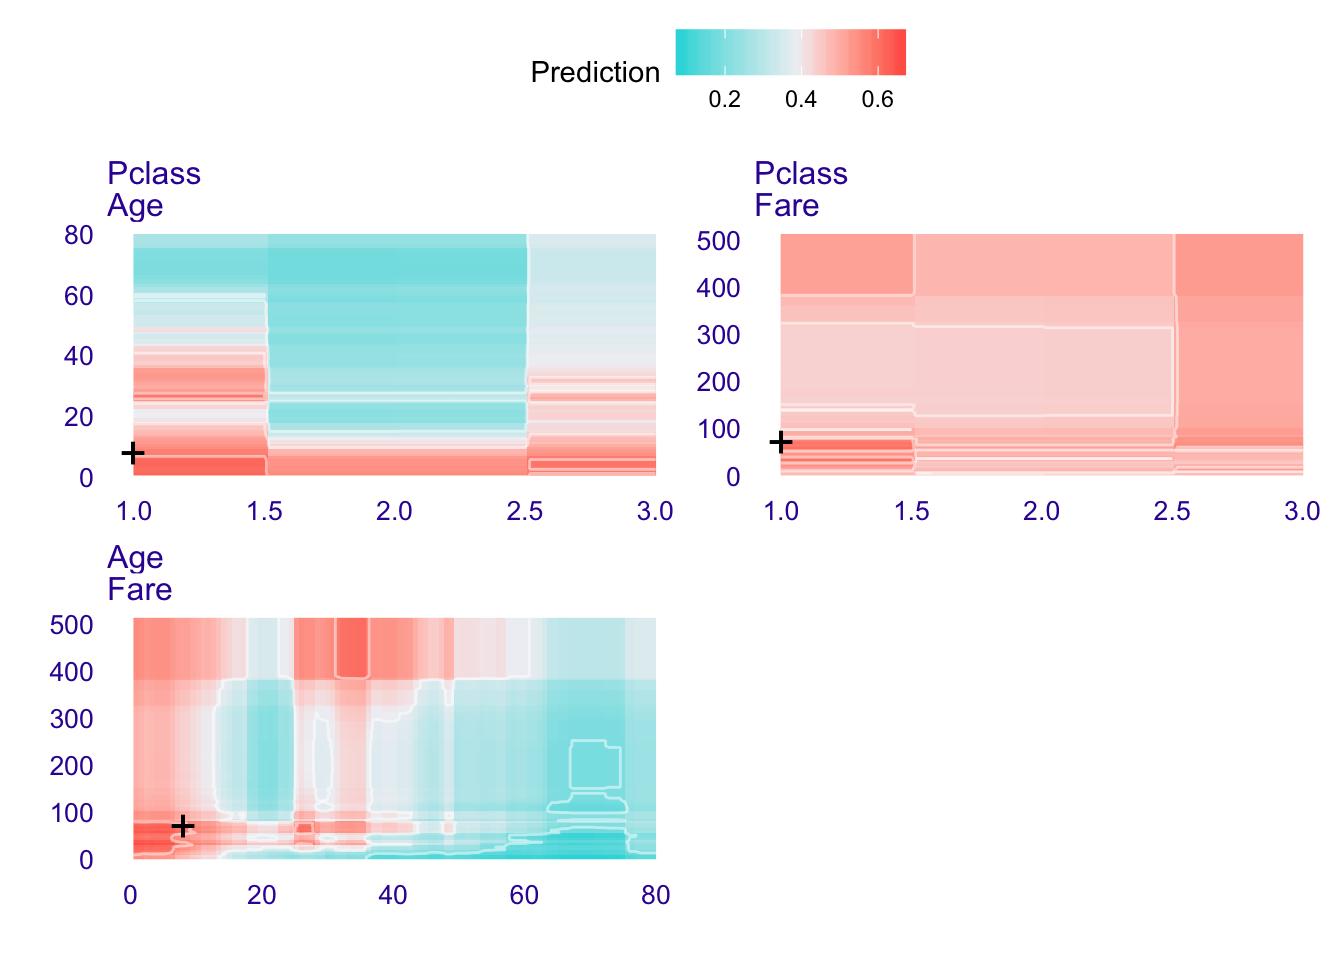
\includegraphics{PM_VEE_files/figure-latex/unnamed-chunk-9-1.pdf}

\hypertarget{break-down-for-interactions}{%
\chapter{Break Down for
Interactions}\label{break-down-for-interactions}}

In the Section \ref{breakDown} we presented model agnostic approach for
additive decomposition of a model prediction for a single observation.

For non-additive models the variables contributions depend on values of
other variables.

In this section we present an algorithm that identifies interactions
between pairs of variables and include such interactions in variable
decomposition plots. Here we present an algorithm for pairs of
variables, but it can be easily generalized to larger number of
variables.

\hypertarget{the-algorithm-1}{%
\section{The Algorithm}\label{the-algorithm-1}}

This algorithm is also composed out of two steps. In the first step
variables and pairs of variables are ordered in terms of their
importance, while in the second step the consecutive conditioning is
applied to ordered variables.

To determine an importance of variables and pairs of variables following
scores are being calculated.

For a single variable

\[
score_1(f, x^*, i) = \left| E [f(X)|X_i = x^*_i]  - E [f(X)]\right|
\] For pairs of variables

\[
score_2(f, x^*, (i,j)) = \left| E [f(X)|X_i = x^*_i, X_j = x^*_j] - E [f(X)|X_i = x^*_i] - E [f(X)| X_j = x^*_j]+ E [f(X)] \right|
\] Note that this is equivalent to

\[
score_2(f, x^*, (i,j)) = \left| E [f(X)|X_i = x^*_i, X_j = x^*_j] - score_1 (f, x^*, i) - score_1 (f, x^*, j) + baseline \right|
\] In other words the \(score_1(f, x^*, i)\) measures how much the
average model response changes if variable \(x_i\) is set to \(x_i^*\),
which is some index of local variable importance. On the other hand the
\(score_2(f, x^*, (i,j))\) measures how much the change is different
than additive composition of changes for \(x_i\) and \(x_j\), which is
some index of local interaction importance.

Note, that for additive models \(score_2(f, x^*, (i,j))\) shall be close
to zero. So the larger is this value the larger deviation from
additivness.

The second step of the algorithm is the sequential conditioning. In this
version in every new step we condition on a single variable of pair of
variables in an order determined by \(score_1\) and \(score_2\).

The complexity of the first step id \(O(p^2)\) where \(p\) stands for
the number of variables. The complexity of the second step is \(O(p)\).

\hypertarget{hr-dataset-hire-or-fire-1}{%
\section{HR dataset: Hire or Fire?}\label{hr-dataset-hire-or-fire-1}}

Again, let us consider a HR dataset. The table below shows \(score_1\)
and \(score_2\) calculated for consecutive variables.

\begin{longtable}[]{@{}lrrr@{}}
\toprule
& Ei f(X) & score1 & score2\tabularnewline
\midrule
\endhead
hours & 0.616200 & 0.230614 &\tabularnewline
salary & 0.225528 & -0.160058 &\tabularnewline
age:gender & 0.516392 & & 0.146660\tabularnewline
salary:age & 0.266226 & & 0.062026\tabularnewline
salary:hours & 0.400206 & & -0.055936\tabularnewline
evaluation & 0.430994 & 0.045408 &\tabularnewline
hours:age & 0.635662 & & 0.040790\tabularnewline
salary:evaluation & 0.238126 & & -0.032810\tabularnewline
age & 0.364258 & -0.021328 &\tabularnewline
evaluation:hours & 0.677798 & & 0.016190\tabularnewline
salary:gender & 0.223292 & & -0.007710\tabularnewline
evaluation:age & 0.415688 & & 0.006022\tabularnewline
gender & 0.391060 & 0.005474 &\tabularnewline
hours:gender & 0.626478 & & 0.004804\tabularnewline
evaluation:gender & 0.433814 & & -0.002654\tabularnewline
\bottomrule
\end{longtable}

Once we determined the order, we can calculate sequential conditionings.
In the first step we condition over variable \texttt{hours}, then over
\texttt{salary}. The third position is occupied by interaction between
\texttt{age:gender} thus we add both variables to the conditioning

\begin{longtable}[]{@{}lrr@{}}
\toprule
variable & cumulative & contribution\tabularnewline
\midrule
\endhead
(Intercept) & 0.385586 & 0.385586\tabularnewline
* hours = 42 & 0.616200 & 0.230614\tabularnewline
* salary = 2 & 0.400206 & -0.215994\tabularnewline
* age:gender = 58:male & 0.796856 & 0.396650\tabularnewline
* evaluation = 2 & 0.778000 & -0.018856\tabularnewline
final\_prognosis & 0.778000 & 0.778000\tabularnewline
\bottomrule
\end{longtable}

\hypertarget{break-down-plots-1}{%
\section{Break Down Plots}\label{break-down-plots-1}}

Break Down Plots for interactions are similar in structure as plots for
single variables. The only difference is that in some rows pair of
variable is listed in a single row. See an example in Figure
\ref{BDPrice4}.

\begin{figure}

{\centering 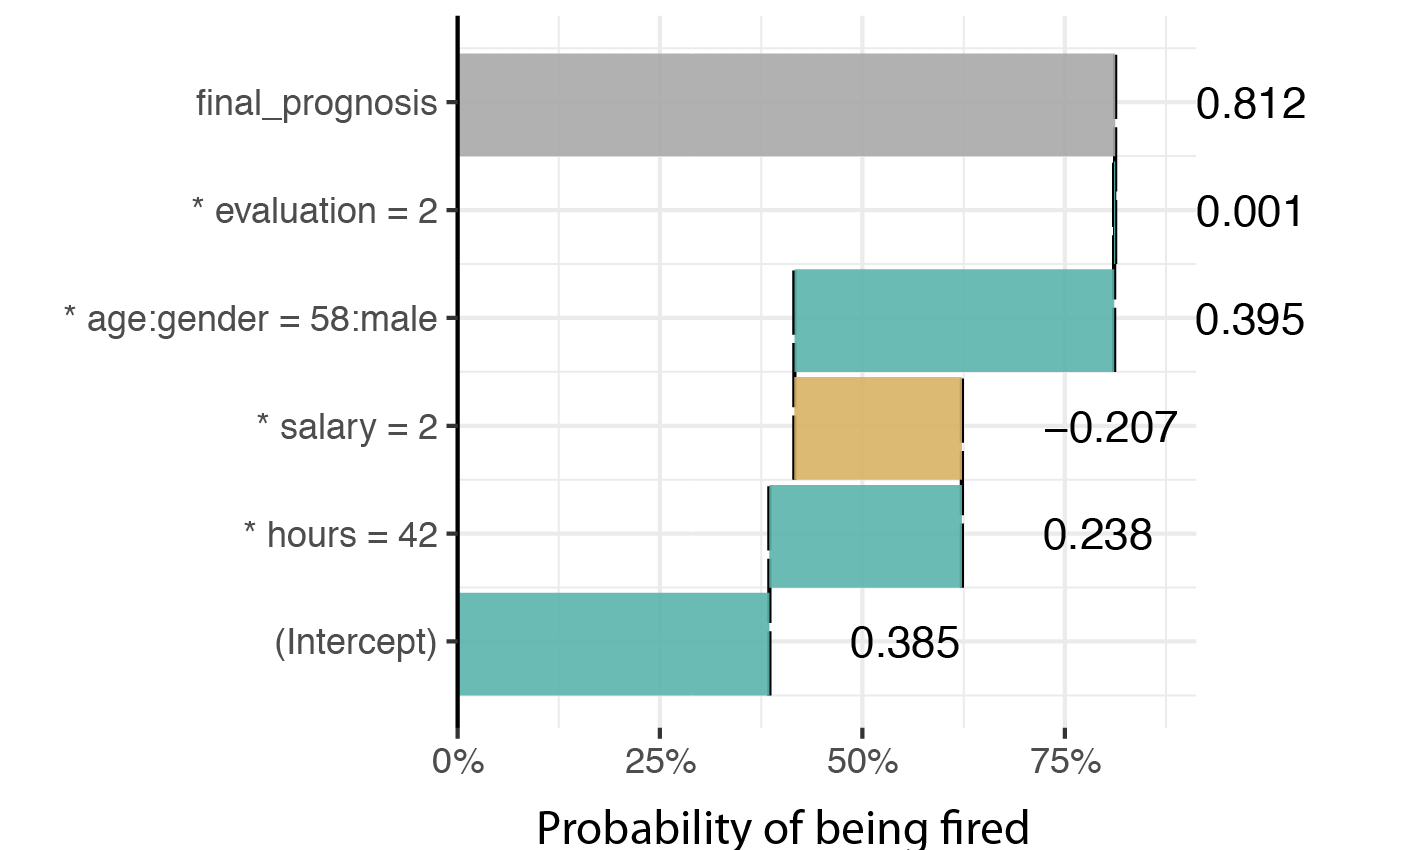
\includegraphics[width=0.7\linewidth]{figure/bd_inter_1} 

}

\caption{(fig:bdInter1) Break Down Plot for variable attrbution with interactions }\label{fig:bdInter1}
\end{figure}

\hypertarget{pros-and-cons-1}{%
\section{Pros and cons}\label{pros-and-cons-1}}

Break Down for interactions shares many features of Break Down for
single variables. Below we summarize unique strengths and weaknesses of
this approach.

\textbf{Pros}

\begin{itemize}
\tightlist
\item
  If interactions are present in the model, then additive contributions
  may be misleading. In such case the identification of interactions
  leads to better explanations.
\item
  Complexity of Break Down Algorithm is quadratic, what is not that bad
  if number of features is small or moderate.
\end{itemize}

\textbf{Cons}

\begin{itemize}
\tightlist
\item
  For large number of variables, the consideration of all interactions
  is both time consuming and sensitive to noise as the number of
  \(score_2\) scores grow faster than number of \(score_1\).
\end{itemize}

\hypertarget{code-snippets-for-r-1}{%
\section{Code snippets for R}\label{code-snippets-for-r-1}}

The algorithm for Break Down for Interactions is also implemented in the
\texttt{break\_down} function from \texttt{breakDown} package.

It is enough to set argument \texttt{check\_interactions\ =\ TRUE} to
identify interactions.

\textbf{Model preparation}

First a model needs to be trained.

\begin{Shaded}
\begin{Highlighting}[]
\KeywordTok{library}\NormalTok{(}\StringTok{"DALEX"}\NormalTok{)}
\KeywordTok{library}\NormalTok{(}\StringTok{"randomForest"}\NormalTok{)}
\NormalTok{model <-}\StringTok{ }\KeywordTok{randomForest}\NormalTok{(status }\OperatorTok{~}\StringTok{ }\NormalTok{gender }\OperatorTok{+}\StringTok{ }\NormalTok{age }\OperatorTok{+}\StringTok{ }\NormalTok{hours }\OperatorTok{+}\StringTok{ }\NormalTok{evaluation }\OperatorTok{+}\StringTok{ }\NormalTok{salary, }\DataTypeTok{data =}\NormalTok{ HR)}
\NormalTok{model}
\end{Highlighting}
\end{Shaded}

\begin{verbatim}
## 
## Call:
##  randomForest(formula = status ~ gender + age + hours + evaluation +      salary, data = HR) 
##                Type of random forest: classification
##                      Number of trees: 500
## No. of variables tried at each split: 2
## 
##         OOB estimate of  error rate: 27.69%
## Confusion matrix:
##          fired   ok promoted class.error
## fired     2256  396      203   0.2098074
## ok         529 1245      447   0.4394417
## promoted   204  394     2173   0.2158066
\end{verbatim}

Model exploration with the \texttt{breakDown} package is performed in
three steps.

\textbf{1. Create an explainer - wrapper around model and validation
data.}

Since all other functions work in a model agnostic fashion, first we
need to define a wrapper around the model. Here we are using the
\texttt{explain()} function from \texttt{DALEX} package.

\begin{Shaded}
\begin{Highlighting}[]
\NormalTok{explainer_rf_fired <-}\StringTok{ }\KeywordTok{explain}\NormalTok{(model,}
                 \DataTypeTok{data =}\NormalTok{ HR,}
                 \DataTypeTok{y =}\NormalTok{ HR}\OperatorTok{$}\NormalTok{status }\OperatorTok{==}\StringTok{ "fired"}\NormalTok{,}
                 \DataTypeTok{predict_function =} \ControlFlowTok{function}\NormalTok{(m,x) }\KeywordTok{predict}\NormalTok{(m,x, }\DataTypeTok{type =} \StringTok{"prob"}\NormalTok{)[,}\DecValTok{1}\NormalTok{],}
                 \DataTypeTok{label =} \StringTok{"fired"}\NormalTok{)}
\end{Highlighting}
\end{Shaded}

\textbf{2. Select an observation of interest.}

Break Down Plots decompose model prediction around a single observation.
Let's construct a data frame with corresponding values.

\begin{Shaded}
\begin{Highlighting}[]
\NormalTok{new_observation <-}\StringTok{ }\KeywordTok{data.frame}\NormalTok{(}\DataTypeTok{gender =} \KeywordTok{factor}\NormalTok{(}\StringTok{"male"}\NormalTok{, }\DataTypeTok{levels =} \KeywordTok{c}\NormalTok{(}\StringTok{"male"}\NormalTok{, }\StringTok{"female"}\NormalTok{)),}
                      \DataTypeTok{age =} \FloatTok{57.7}\NormalTok{,}
                      \DataTypeTok{hours =} \FloatTok{42.3}\NormalTok{,}
                      \DataTypeTok{evaluation =} \DecValTok{2}\NormalTok{,}
                      \DataTypeTok{salary =} \DecValTok{2}\NormalTok{)}

\KeywordTok{predict}\NormalTok{(model, new_observation, }\DataTypeTok{type =} \StringTok{"prob"}\NormalTok{)}
\end{Highlighting}
\end{Shaded}

\begin{verbatim}
##   fired    ok promoted
## 1 0.814 0.186        0
## attr(,"class")
## [1] "matrix" "votes"
\end{verbatim}

\textbf{3. Calculate Break Down decomposition}

The \texttt{break\_down()} function calculates Break Down contributions
for a selected model around a selected observation.

Note that \texttt{check\_interactions\ =\ TRUE} is needed to identify
interactions.

The result from \texttt{break\_down()} function is a data frame with
variable attributions.

\begin{Shaded}
\begin{Highlighting}[]
\KeywordTok{library}\NormalTok{(}\StringTok{"breakDown"}\NormalTok{)}
\NormalTok{bd_rf <-}\StringTok{ }\KeywordTok{break_down}\NormalTok{(explainer_rf_fired,}
\NormalTok{                 new_observation,}
                 \DataTypeTok{check_interactions =} \OtherTok{TRUE}\NormalTok{)}

\NormalTok{bd_rf}
\end{Highlighting}
\end{Shaded}

\begin{verbatim}
##                        contribution
## (Intercept)                   0.375
## * hours = 42                  0.235
## * salary = 2                 -0.208
## * age:gender = 58:male        0.404
## * evaluation = 2              0.008
## final_prognosis               0.814
## baseline:  0
\end{verbatim}

The generic \texttt{plot()} function creates a Break Down plots.

\begin{Shaded}
\begin{Highlighting}[]
\KeywordTok{plot}\NormalTok{(bd_rf) }
\end{Highlighting}
\end{Shaded}

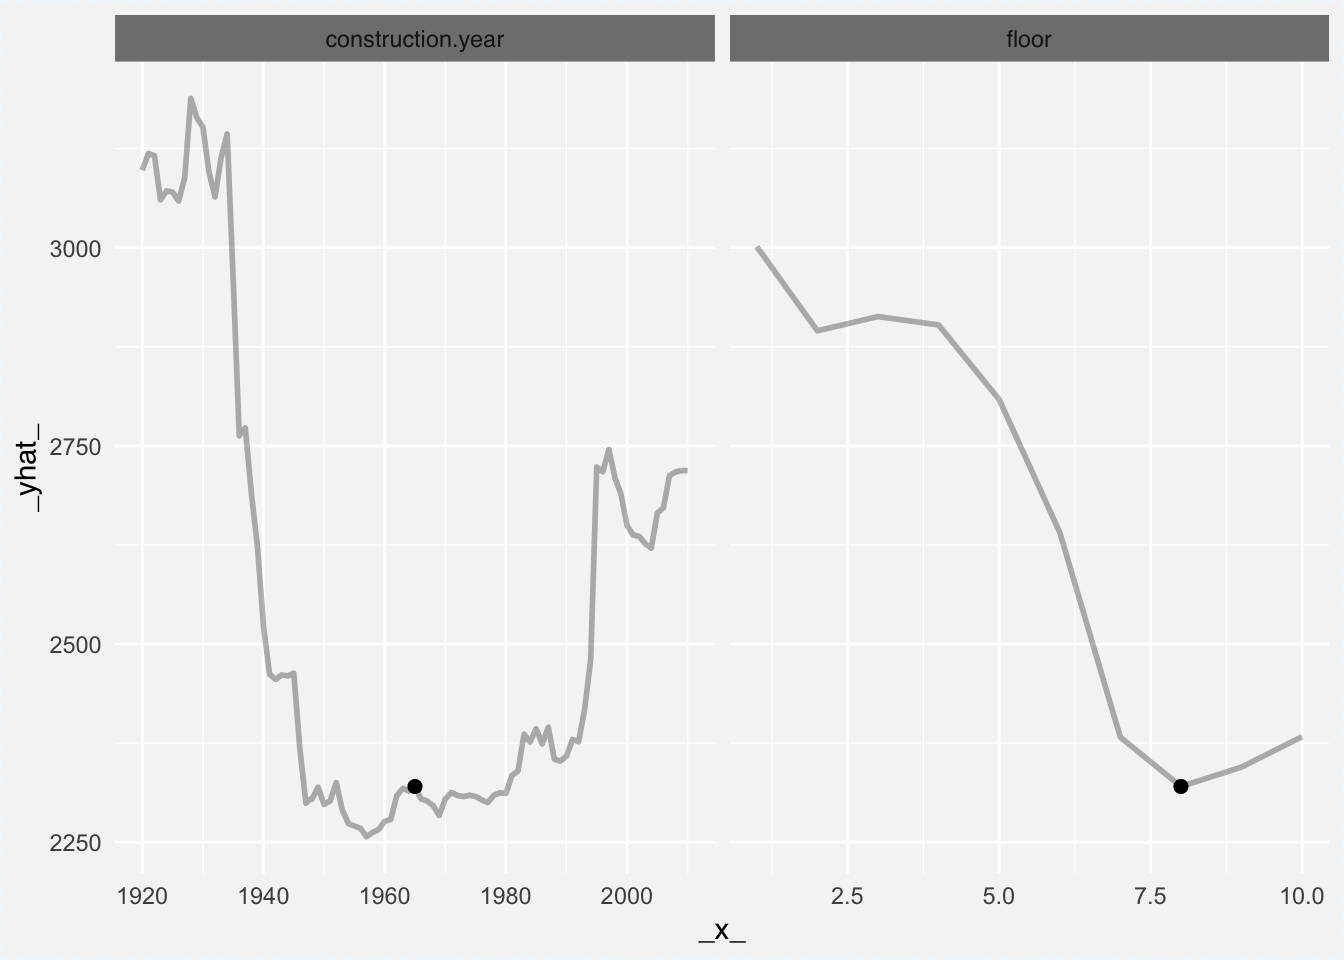
\includegraphics{PM_VEE_files/figure-latex/unnamed-chunk-15-1.pdf}

\hypertarget{shapley}{%
\chapter{Shapley Attributions}\label{shapley}}

In the Section \ref{modelAgnosticAttribution} we show the problem
related to the ordering of variables. In the Section \ref{breakDown} we
show an approach in which the ordering was determined based on single
step assessment of variable importance.

In this section we introduce other, very popular approach for additive
variable attribution. The problem of contributions that depends on the
variable ordering is solved by averaging over all possible orderings.

This method is motivated with results in cooperative game theory and was
first introduced in \citep{Strumbelj2014}. Wide adoption of this method
comes with a NIPS 2017 paper \citep{SHAP} and python library SHAP
\texttt{https://github.com/slundberg/shap}. Authors of the SHAP method
introduced also efficient algorithm for tree-based models, see
\citep{TreeSHAP}.

\hypertarget{the-algorithm-2}{%
\section{The Algorithm}\label{the-algorithm-2}}

The name \emph{Shapley Values} comes from the solution in cooperative
game theory attributed to Lloyd Shapley. The original problem was to
assess how important is each player to the overall cooperation, and what
payoff can he or she reasonably expect from the coalition?
\citep{shapleybook1952}

In the context of model interpretability the payoff is the average model
response while the players are the variables in the conditioning. Then
Formula for variable contributions is following.

\[
v(f, x^*, i) = \frac 1{|P|}\sum_{S \subseteq P\setminus \{i\}}  {{|P|-1}\choose{|S|}}^{-1} \left(E [f(X) | X_{S \cup \{i\}} = x^*_{S \cup \{i\}}] - E [f(X) | X_{S} = x^*_{S}]\right)
\] where \(P = \{1, \ldots, p\}\) is the set of all variables. The
intuition beyond this contribution is following. We consider all
possible orderings of variables (yes, there is \(2^p\) of them) and
calculate the contribution of variable \(i\) as an average from
contributions calculated in particular orderings.

The part
\(E[f(X) | X_{S \cup \{i\}} = x^*_{S \cup \{i\}}] - E [f(X) | X_{S} = x^*_{S}]\)
is the contribution of variable \(i\) which is introduces after
variables from \(S\).

Time complexity of this method is \(O(2^p)\) where \(p\) stands for the
number of variables. Such complexity makes this method impractical for
most cases. Fortunately it is enough to assess this value.
\citep{Strumbelj2014} proposed to use sampling. \citep{TreeSHAP}
proposed fast implementations for tree based ensembles.

\hypertarget{code-snippets-for-r-2}{%
\section{Code snippets for R}\label{code-snippets-for-r-2}}

In this section we will present an example based on the \texttt{HR}
dataset and Random Forest model \citep{R-randomForest}. See the Section
\ref{HRdataset} for more details.

\begin{Shaded}
\begin{Highlighting}[]
\KeywordTok{library}\NormalTok{(}\StringTok{"DALEX"}\NormalTok{)}
\KeywordTok{library}\NormalTok{(}\StringTok{"randomForest"}\NormalTok{)}
\NormalTok{model_rf <-}\StringTok{ }\KeywordTok{randomForest}\NormalTok{(status }\OperatorTok{~}\StringTok{ }\NormalTok{gender }\OperatorTok{+}\StringTok{ }\NormalTok{age }\OperatorTok{+}\StringTok{ }\NormalTok{hours }\OperatorTok{+}\StringTok{ }\NormalTok{evaluation }\OperatorTok{+}\StringTok{ }\NormalTok{salary, }\DataTypeTok{data =}\NormalTok{ HR)}
\end{Highlighting}
\end{Shaded}

Here we use the \texttt{iml} package, see more examples in
\citep{imlPackage}.

\begin{Shaded}
\begin{Highlighting}[]
\KeywordTok{library}\NormalTok{(}\StringTok{"iml"}\NormalTok{)}
\NormalTok{explainer_rf =}\StringTok{ }\NormalTok{Predictor}\OperatorTok{$}\KeywordTok{new}\NormalTok{(model_rf, }\DataTypeTok{data =}\NormalTok{ HR, }\DataTypeTok{type=}\StringTok{"prob"}\NormalTok{)}
\end{Highlighting}
\end{Shaded}

Explanations for a new observation.

\begin{Shaded}
\begin{Highlighting}[]
\NormalTok{new_observation <-}\StringTok{ }\KeywordTok{data.frame}\NormalTok{(}\DataTypeTok{gender =} \KeywordTok{factor}\NormalTok{(}\StringTok{"male"}\NormalTok{, }\DataTypeTok{levels =} \KeywordTok{c}\NormalTok{(}\StringTok{"male"}\NormalTok{, }\StringTok{"female"}\NormalTok{)),}
                      \DataTypeTok{age =} \FloatTok{57.7}\NormalTok{,}
                      \DataTypeTok{hours =} \FloatTok{42.3}\NormalTok{,}
                      \DataTypeTok{evaluation =} \DecValTok{2}\NormalTok{,}
                      \DataTypeTok{salary =} \DecValTok{2}\NormalTok{,}
                      \DataTypeTok{status =} \KeywordTok{factor}\NormalTok{(}\StringTok{"fired"}\NormalTok{))}

\NormalTok{shapley =}\StringTok{ }\NormalTok{Shapley}\OperatorTok{$}\KeywordTok{new}\NormalTok{(explainer_rf, }\DataTypeTok{x.interest =}\NormalTok{ new_observation)}
\NormalTok{shapley}
\end{Highlighting}
\end{Shaded}

\begin{verbatim}
## Interpretation method:  Shapley 
## Predicted value: 0.792000, Average prediction: 0.376076 (diff = 0.415924) Predicted value: 0.204000, Average prediction: 0.274359 (diff = -0.070359) Predicted value: 0.004000, Average prediction: 0.349564 (diff = -0.345564)
## 
## Analysed predictor: 
## Prediction task: unknown 
## 
## 
## Analysed data:
## Sampling from data.frame with 7847 rows and 6 columns.
## 
## Head of results:
##      feature class      phi    phi.var feature.value
## 1     gender fired  0.09432 0.05763190   gender=male
## 2        age fired  0.15054 0.07755199      age=57.7
## 3      hours fired  0.32418 0.11445657    hours=42.3
## 4 evaluation fired  0.01776 0.01954709  evaluation=2
## 5     salary fired -0.11878 0.03188193      salary=2
## 6     status fired  0.00000 0.00000000  status=fired
\end{verbatim}

And the plot with Shapley attributions.

\begin{Shaded}
\begin{Highlighting}[]
\KeywordTok{plot}\NormalTok{(shapley)}
\end{Highlighting}
\end{Shaded}

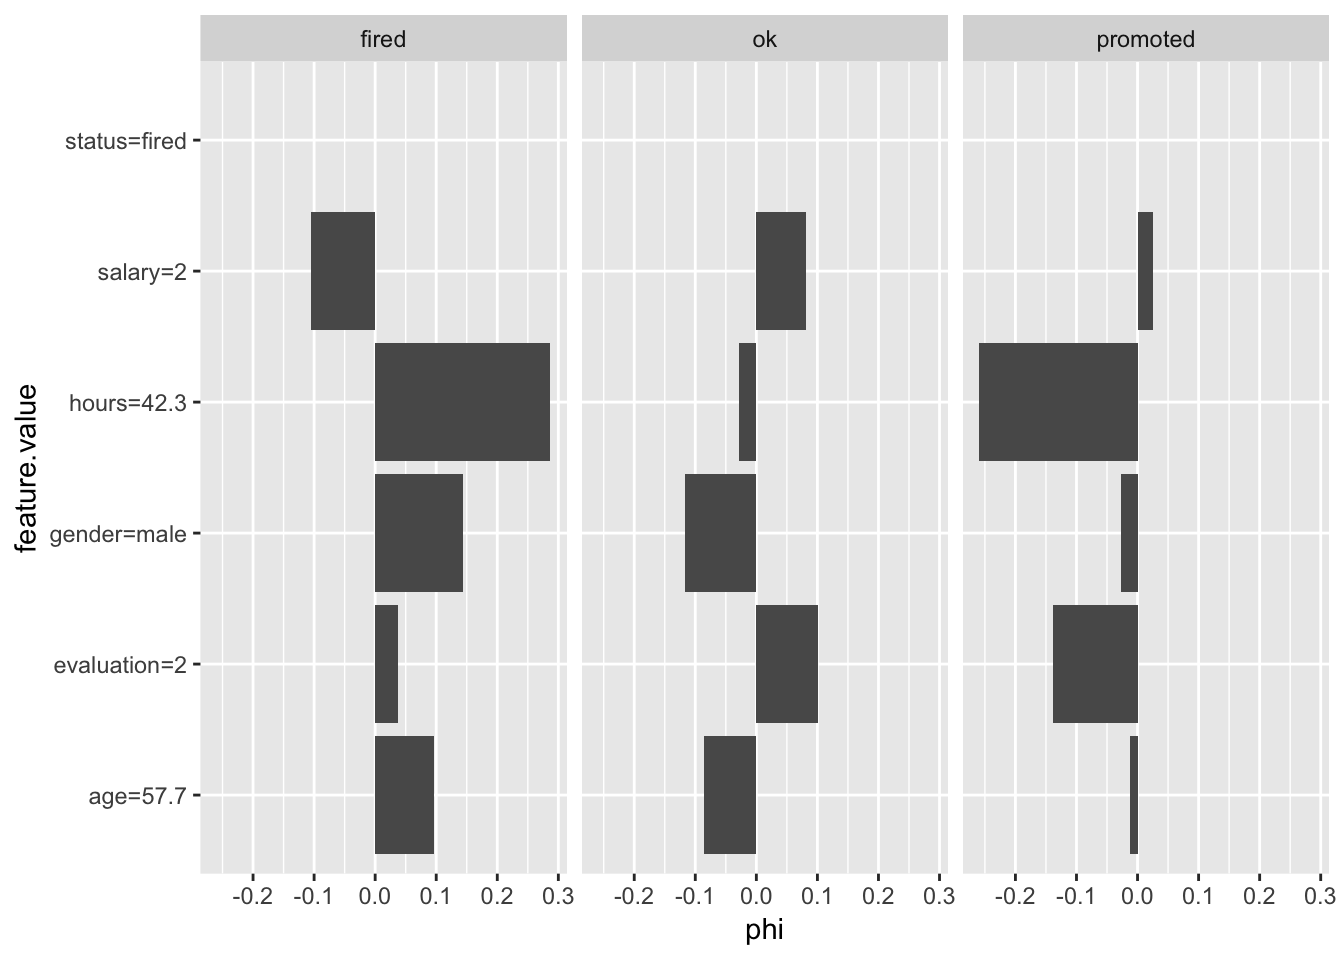
\includegraphics{PM_VEE_files/figure-latex/unnamed-chunk-19-1.pdf}

See more examples for \texttt{iml} package in the \citep{molnar} book.

\hypertarget{pros-and-cons-2}{%
\section{Pros and cons}\label{pros-and-cons-2}}

Shapley Values give a uniform approach to decompose model prediction
into parts that can be attributed additively to variables. Below we
summarize key strengths and weaknesses of this approach.

\textbf{Pros}

\begin{itemize}
\tightlist
\item
  There is a nice theory based on cooperative games.
\item
  \citep{SHAP} shows that this method unifies different approaches to
  additive features attribution.
\item
  There is efficient implementation available for Python.
\item
  \citep{SHAP} shows more desired properties of this method, like
  symmetry or additivity.
\end{itemize}

\textbf{Cons}

\begin{itemize}
\tightlist
\item
  The exact calculation of Shapley values is time consuming.
\item
  If the model is not additive, then the Shaply scores may be
  misleading. And there is no way to determine if model is far from
  additiveness.
\end{itemize}

Note that fully additive model solutions presented in sections
\ref{modelAgnosticAttribution}, \ref{breakDown} and \ref{shapley} lead
to same variable contributions.

\hypertarget{LIME}{%
\chapter{Local approximations with white-box model}\label{LIME}}

A different approach to explanations of a single observations is through
surrogate models. Models that easy to understand and are similar to
black box model around the point of interest.

Variable attribution methods, that were presented in the Section
\ref{breakDown} are not interested in the local curvature of the model.
They rather compare model prediction against average model prediction
and they use probability structure of the dataset.

The complementary approach would be to directly explore information
about model curvature around point of interest. In the section
\ref{ceterisParibus} we introduced Ceteris Paribus tool for such what-if
analysis. But the limitation of ceteris Paribus pltos is that they
explore changes along single dimension or pairs of dimensions.

In this section we describe an another approach based on local
approximations with white-box models. This approach will also
investigate local curvature of the model but indirectly, through
surrogate white-box models.

The most known method from this class if LIME (Local Interpretable
Model-Agnostic Explanations), introduced in the paper \emph{Why Should I
Trust You?: Explaining the Predictions of Any Classifier} \citep{lime}.
This methods and it's clones are now implemented in various R and python
packages, see for example \citep{R-lime}, \citep{R-live} or
\citep{R-iml}.

\hypertarget{the-algorithm-3}{%
\section{The Algorithm}\label{the-algorithm-3}}

The LIME method, and its clones, has following properties:

\begin{itemize}
\tightlist
\item
  \emph{model-agnostic}, they do not imply any assumptions on model
  structure,
\item
  \emph{interpretable representation}, model input is transformed into a
  feature space that is easier to understand. One of applications comes
  from image data, single pixels are not easy to interpret, thus the
  LIME method decompose image into a series of super pixels, that are
  easier to interpret to humans,
\item
  \emph{local fidelity} means that the explanations shall be locally
  well fitted to the black-box model.
\end{itemize}

Therefore the objective is to find a local model \(M^L\) that
approximates the black box model \(f\) in the point \(x^*\). As a
solution the penalized loss function is used. The white-box model that
is used for explanations satisfies following condition.

\[
M^L(x^*) = \arg \min_{g \in G} L(f, g, \Pi_{x^*}) + \Omega (g) 
\] where \(G\) is a family of white box models (e.g.~linear models),
\(\Pi_{x^*}\) is neighbourhood of \(x^*\) and \(\Omega\) stands for
model complexity.

\begin{figure}

{\centering 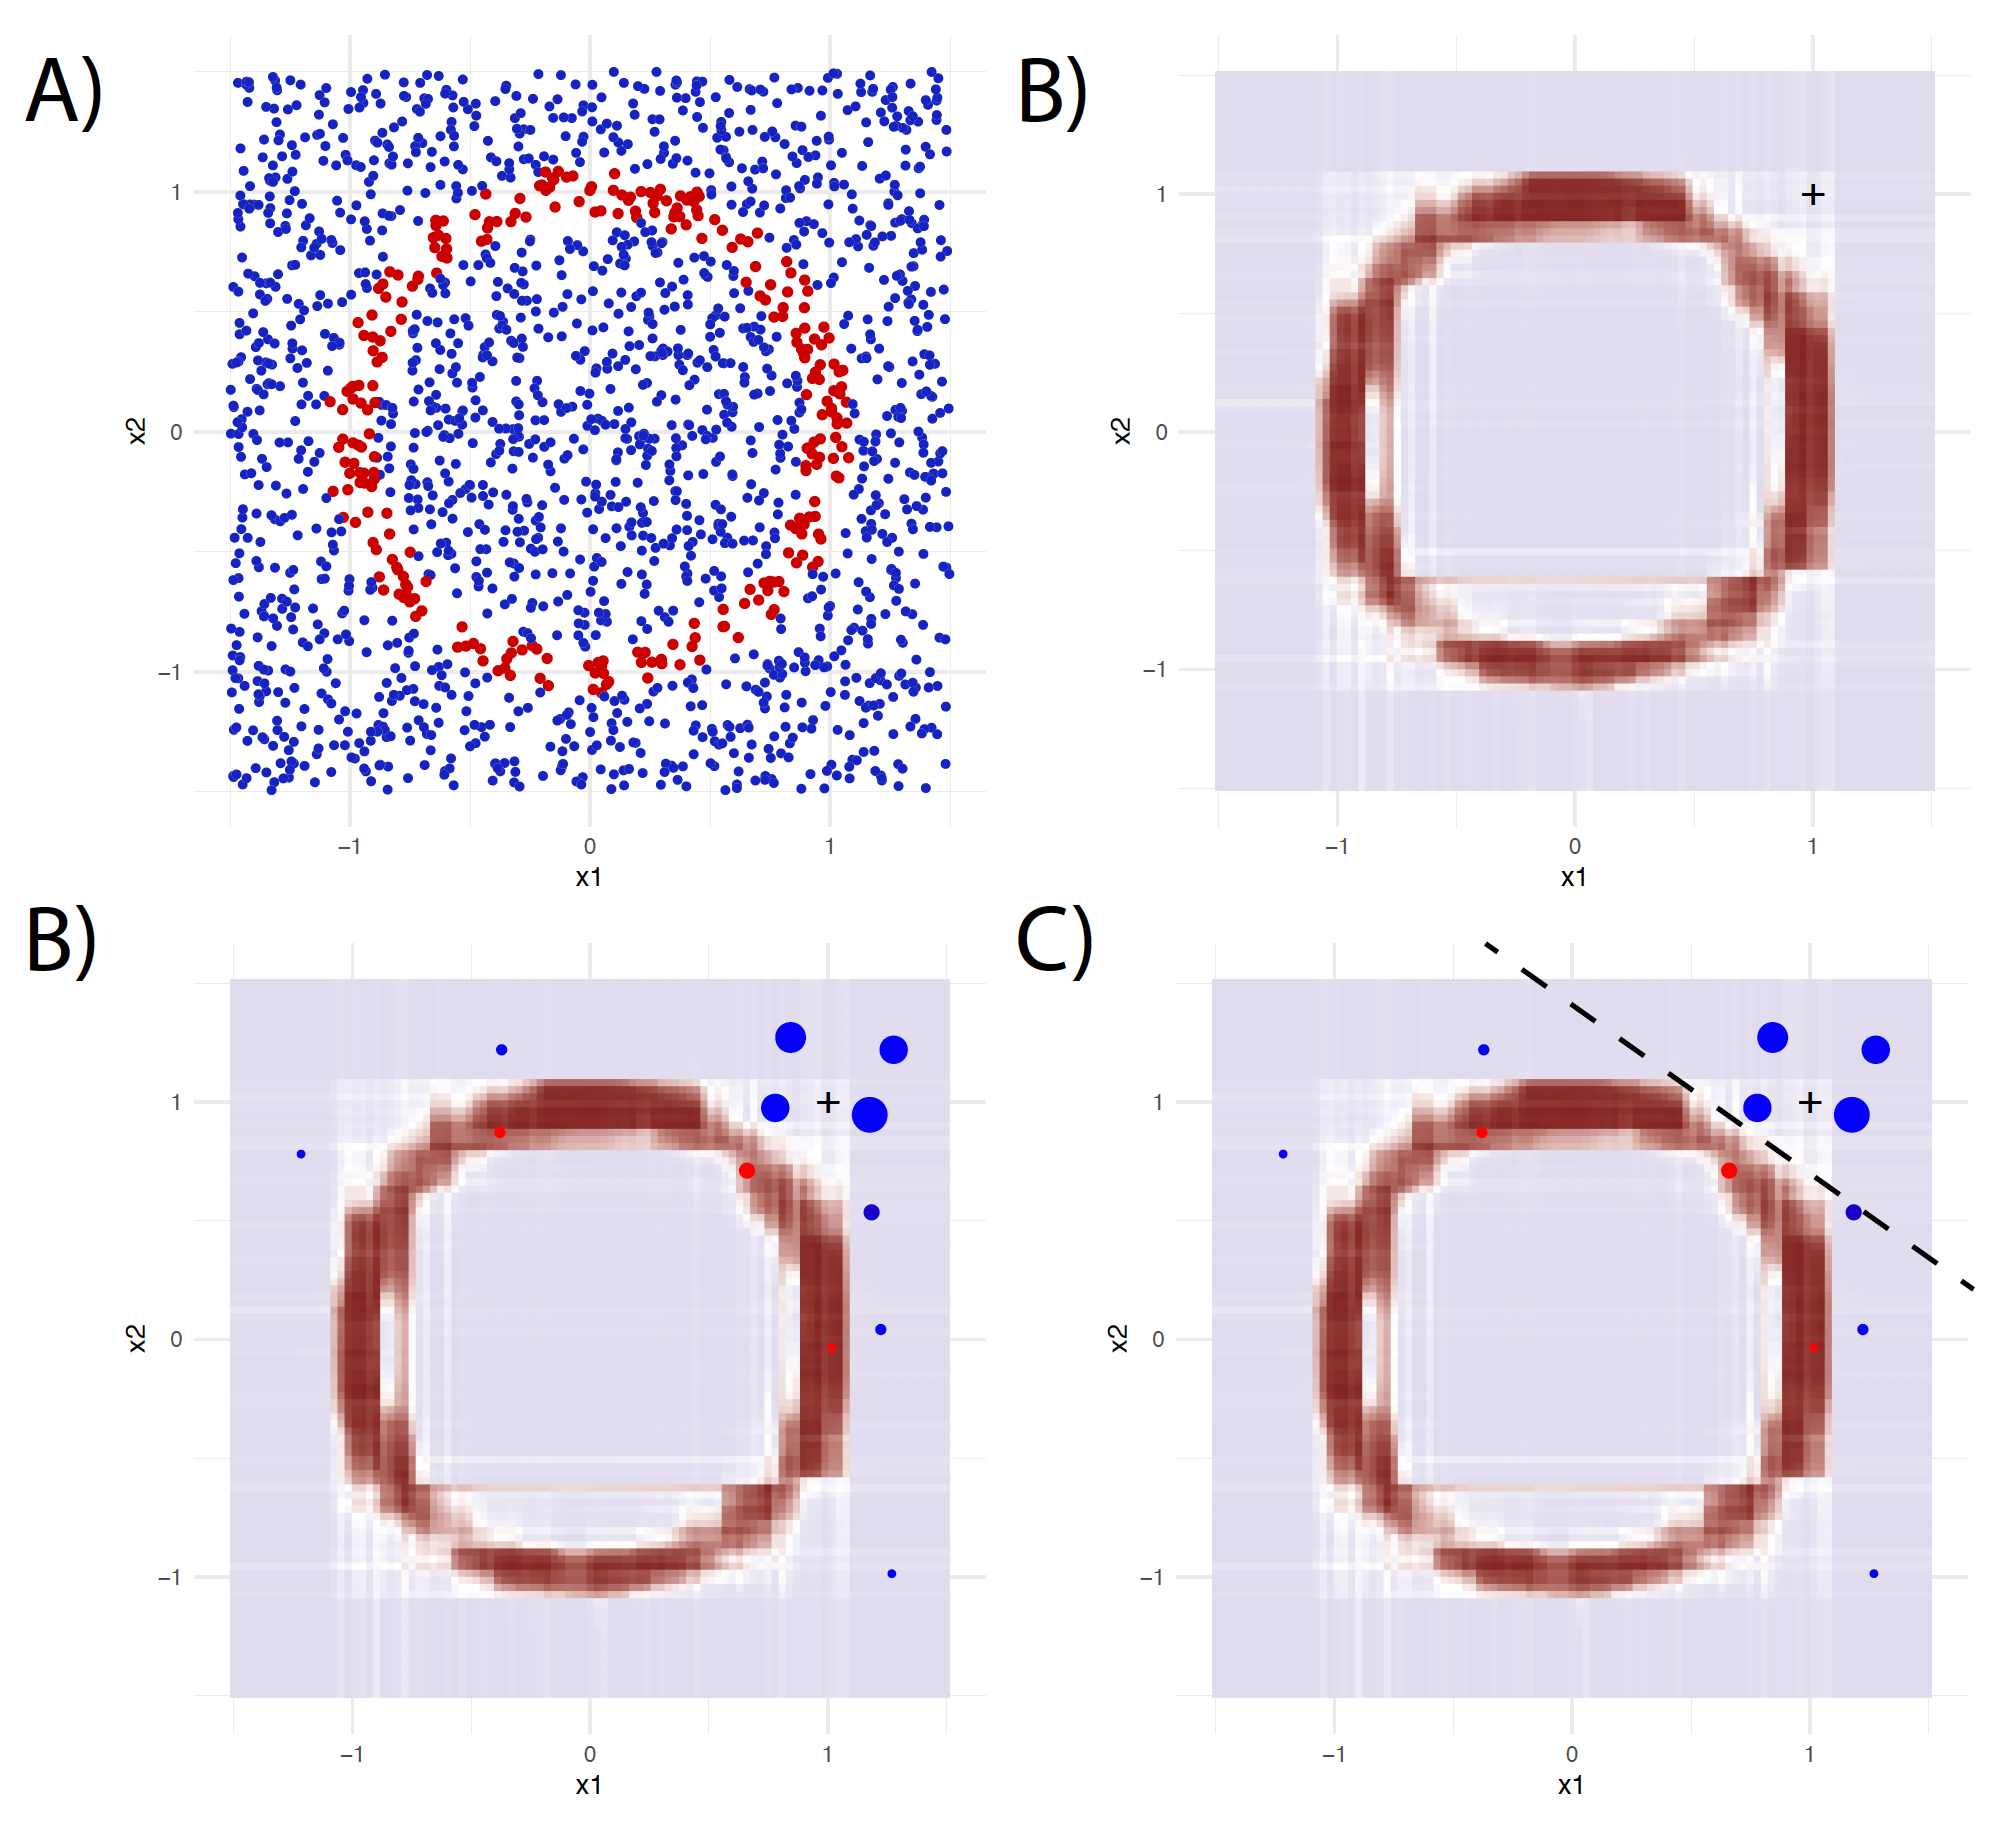
\includegraphics[width=0.7\linewidth]{figure/circle_4panels} 

}

\caption{(fig:LIME1) A schematic idea behind local model approximations. Panel A shows training data, colors correspond to classess. Panel B showhs results fom the Random Forest model, whis is where the algorithm starts. Panel C shows new data sampled around the point of interest. Their color correspond to model response. Panel D shows fitted linear model that approximated the random forest model around point of interest}\label{fig:LIME1}
\end{figure}

The algorithm is composed from three steps:

\begin{itemize}
\tightlist
\item
  Identification of interpretable data representations,
\item
  Local sampling around the point of interest,
\item
  Fitting a white box model in this neighbouhood
\end{itemize}

\textbf{Identification of interpretable data representations}

For image data, single pixel is not an interpretable feature. In this
step the input space of the model is transformed to input space that is
easier to understand for human. The image may be decomposed into parts
and represented as presence/absence of some part of an image.

\textbf{Local sampling around the point of interest}

Once the interpretable data representation is identified, then the
neighbourhood around point of interest needs to be explored.

\textbf{Fitting a white box model in this neighbouhood}

Any model that is easy to interpret may be fitted to this data, like
decision tree or rule based system. However in practice the most common
family of models are linear models.

\hypertarget{hr-dataset-hire-or-fire-2}{%
\section{HR dataset: Hire or Fire?}\label{hr-dataset-hire-or-fire-2}}

\hypertarget{pros-and-cons-3}{%
\section{Pros and cons}\label{pros-and-cons-3}}

Local approximations are model agnostic, can be applied to any
predictive model. Below we summarize key strengths and weaknesses of
this approach.

\textbf{Pros}

\begin{itemize}
\tightlist
\item
  This method is highly adopted in text analysis and image analysis, in
  part thanks to the interpretable data representations.
\item
  The intuition behind the model is straightforward
\item
  Model explanations are sparse, thus only small number of features is
  used
\end{itemize}

\textbf{Cons}

\begin{itemize}
\tightlist
\item
  For continuous variables and tabular data it is not that easy to find
  interpretable representations
\item
  The black-box model approximated the data and the white box model
  approximates the black box model. We do not have control over the
  quality of local fit of the white box model, thus the surrogate model
  may be misleading.
\item
  Due to the \emph{curse of dimensionality}, for high dimensional space
  points are sparse.
\end{itemize}

\hypertarget{code-snippets-for-r-3}{%
\section{Code snippets for R}\label{code-snippets-for-r-3}}

In this section we present example application of \texttt{lime}
\citep{R-lime} and \texttt{live} \citep{R-live} packages. Note that this
method is also implemented in \texttt{iml} \citep{R-iml} and other
packages. These pacakages differ in some details and also results in
different explanations.

\textbf{Model preparation}

In this section we will present examples based on the \texttt{HR}
dataset. See the Section \ref{HRdataset} for more details.

\begin{Shaded}
\begin{Highlighting}[]
\KeywordTok{library}\NormalTok{(}\StringTok{"DALEX"}\NormalTok{)}
\KeywordTok{head}\NormalTok{(HR)}
\end{Highlighting}
\end{Shaded}

\begin{verbatim}
##   gender      age    hours evaluation salary   status
## 1   male 32.58267 41.88626          3      1    fired
## 2 female 41.21104 36.34339          2      5    fired
## 3   male 37.70516 36.81718          3      0    fired
## 4 female 30.06051 38.96032          3      2    fired
## 5   male 21.10283 62.15464          5      3 promoted
## 6   male 40.11812 69.53973          2      0    fired
\end{verbatim}

The problem here is to predict average price for square meter for an
apartment. Let's build a random forest model with \texttt{randomForest}
package \citep{R-randomForest}.

\begin{Shaded}
\begin{Highlighting}[]
\KeywordTok{library}\NormalTok{(}\StringTok{"randomForest"}\NormalTok{)}
\NormalTok{rf_model <-}\StringTok{ }\KeywordTok{randomForest}\NormalTok{(status }\OperatorTok{~}\StringTok{ }\NormalTok{gender }\OperatorTok{+}\StringTok{ }\NormalTok{age }\OperatorTok{+}\StringTok{ }\NormalTok{hours }\OperatorTok{+}\StringTok{ }\NormalTok{evaluation }\OperatorTok{+}\StringTok{ }\NormalTok{salary, }\DataTypeTok{data =}\NormalTok{ HR)}
\NormalTok{rf_model}
\end{Highlighting}
\end{Shaded}

\begin{verbatim}
## 
## Call:
##  randomForest(formula = status ~ gender + age + hours + evaluation +      salary, data = HR) 
##                Type of random forest: classification
##                      Number of trees: 500
## No. of variables tried at each split: 2
## 
##         OOB estimate of  error rate: 27.26%
## Confusion matrix:
##          fired   ok promoted class.error
## fired     2272  384      199   0.2042032
## ok         534 1252      435   0.4362900
## promoted   202  385     2184   0.2118369
\end{verbatim}

\begin{Shaded}
\begin{Highlighting}[]
\NormalTok{new_observation <-}\StringTok{ }\KeywordTok{data.frame}\NormalTok{(}\DataTypeTok{gender =} \KeywordTok{factor}\NormalTok{(}\StringTok{"male"}\NormalTok{, }\DataTypeTok{levels =} \KeywordTok{c}\NormalTok{(}\StringTok{"male"}\NormalTok{, }\StringTok{"female"}\NormalTok{)),}
                      \DataTypeTok{age =} \FloatTok{57.7}\NormalTok{,}
                      \DataTypeTok{hours =} \FloatTok{42.3}\NormalTok{,}
                      \DataTypeTok{evaluation =} \DecValTok{2}\NormalTok{,}
                      \DataTypeTok{salary =} \DecValTok{2}\NormalTok{)}

\KeywordTok{predict}\NormalTok{(rf_model, new_observation, }\DataTypeTok{type =} \StringTok{"prob"}\NormalTok{)}
\end{Highlighting}
\end{Shaded}

\begin{verbatim}
##   fired    ok promoted
## 1 0.796 0.204        0
## attr(,"class")
## [1] "matrix" "votes"
\end{verbatim}

\hypertarget{the-lime-pacakge}{%
\subsection{\texorpdfstring{\textbf{The lime
pacakge}}{The lime pacakge}}\label{the-lime-pacakge}}

\begin{Shaded}
\begin{Highlighting}[]
\KeywordTok{library}\NormalTok{(}\StringTok{"lime"}\NormalTok{)}
\NormalTok{model_type.randomForest <-}\StringTok{ }\ControlFlowTok{function}\NormalTok{(x, ...) }\StringTok{"classification"}
\NormalTok{lime_rf <-}\StringTok{ }\KeywordTok{lime}\NormalTok{(HR[,}\DecValTok{1}\OperatorTok{:}\DecValTok{5}\NormalTok{], rf_model)}
\NormalTok{explanations <-}\StringTok{ }\NormalTok{lime}\OperatorTok{::}\KeywordTok{explain}\NormalTok{(new_observation[,}\DecValTok{1}\OperatorTok{:}\DecValTok{5}\NormalTok{], lime_rf, }\DataTypeTok{n_labels =} \DecValTok{3}\NormalTok{, }\DataTypeTok{n_features =} \DecValTok{3}\NormalTok{)}
\NormalTok{explanations}
\end{Highlighting}
\end{Shaded}

\begin{verbatim}
##       model_type case    label label_prob  model_r2 model_intercept
## 1 classification    1    fired      0.796 0.1273060       0.2538570
## 2 classification    1    fired      0.796 0.1273060       0.2538570
## 3 classification    1    fired      0.796 0.1273060       0.2538570
## 4 classification    1       ok      0.204 0.1318758       0.1917906
## 5 classification    1       ok      0.204 0.1318758       0.1917906
## 6 classification    1       ok      0.204 0.1318758       0.1917906
## 7 classification    1 promoted      0.000 0.2920459       0.5248033
## 8 classification    1 promoted      0.000 0.2920459       0.5248033
## 9 classification    1 promoted      0.000 0.2920459       0.5248033
##   model_prediction    feature feature_value feature_weight
## 1      0.619009536        age          57.7  -0.0039896535
## 2      0.619009536      hours          42.3   0.2562192630
## 3      0.619009536 evaluation           2.0   0.1129229692
## 4      0.471041378        age          57.7   0.0008047738
## 5      0.471041378 evaluation           2.0   0.2098929527
## 6      0.471041378     salary           2.0   0.0685530104
## 7      0.007980027        age          57.7   0.0043845072
## 8      0.007980027 evaluation           2.0  -0.3228860741
## 9      0.007980027      hours          42.3  -0.1983216890
##           feature_desc                      data          prediction
## 1           50.0 < age 2.0, 57.7, 42.3, 2.0, 2.0 0.796, 0.204, 0.000
## 2 37.6 < hours <= 46.3 2.0, 57.7, 42.3, 2.0, 2.0 0.796, 0.204, 0.000
## 3      evaluation <= 3 2.0, 57.7, 42.3, 2.0, 2.0 0.796, 0.204, 0.000
## 4           50.0 < age 2.0, 57.7, 42.3, 2.0, 2.0 0.796, 0.204, 0.000
## 5      evaluation <= 3 2.0, 57.7, 42.3, 2.0, 2.0 0.796, 0.204, 0.000
## 6      1 < salary <= 2 2.0, 57.7, 42.3, 2.0, 2.0 0.796, 0.204, 0.000
## 7           50.0 < age 2.0, 57.7, 42.3, 2.0, 2.0 0.796, 0.204, 0.000
## 8      evaluation <= 3 2.0, 57.7, 42.3, 2.0, 2.0 0.796, 0.204, 0.000
## 9 37.6 < hours <= 46.3 2.0, 57.7, 42.3, 2.0, 2.0 0.796, 0.204, 0.000
\end{verbatim}

\begin{Shaded}
\begin{Highlighting}[]
\KeywordTok{plot_features}\NormalTok{(explanations)}
\end{Highlighting}
\end{Shaded}

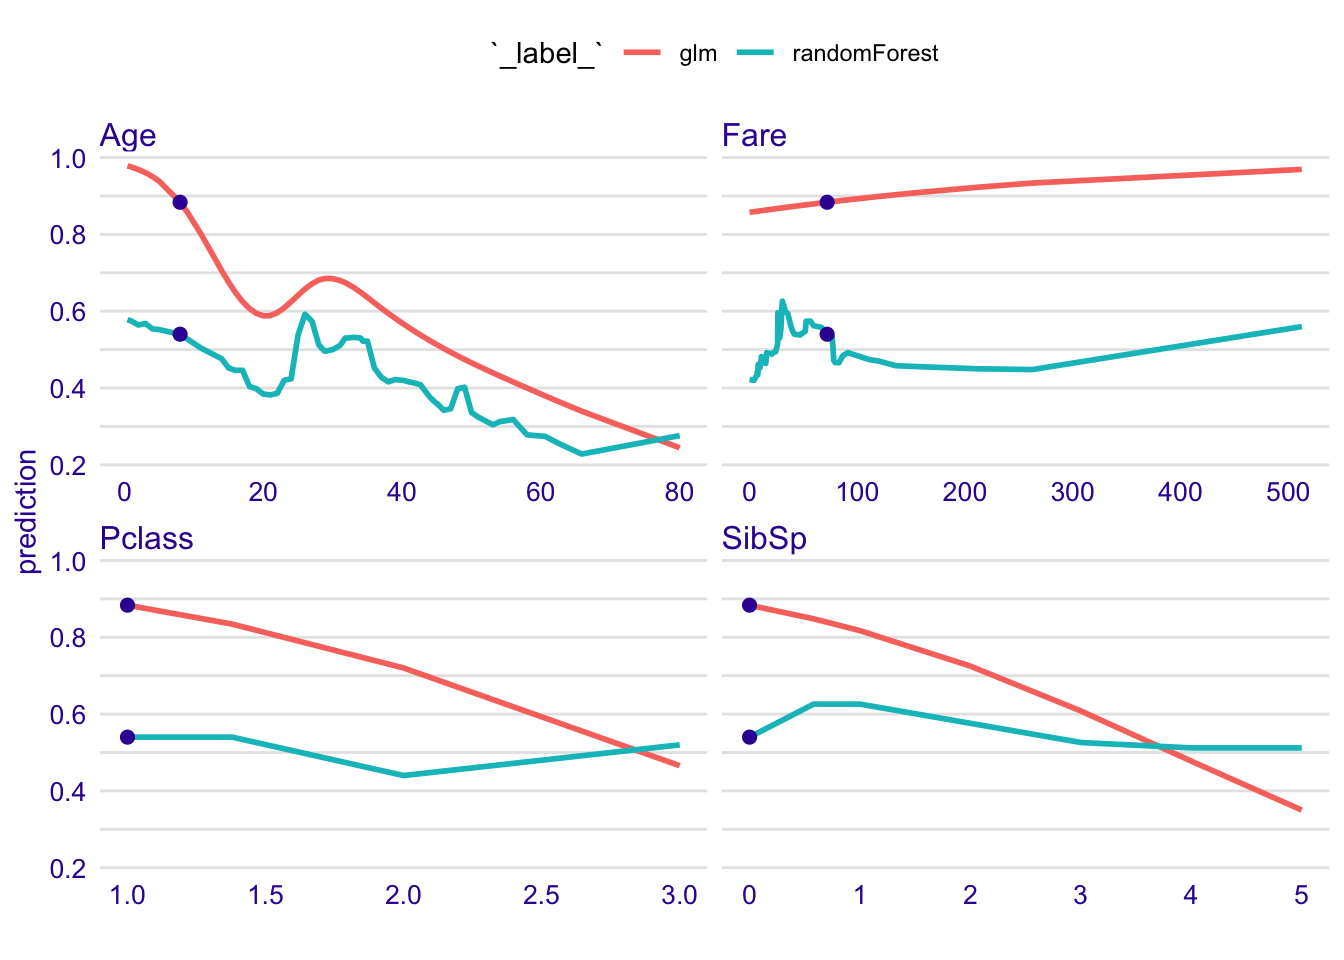
\includegraphics{PM_VEE_files/figure-latex/unnamed-chunk-24-1.pdf}

\hypertarget{the-live-package}{%
\subsection{\texorpdfstring{\textbf{The live
package}}{The live package}}\label{the-live-package}}

\begin{Shaded}
\begin{Highlighting}[]
\KeywordTok{library}\NormalTok{(}\StringTok{"live"}\NormalTok{)}

\NormalTok{new_observation}\OperatorTok{$}\NormalTok{status <-}\StringTok{ "fired"}
\NormalTok{explainer_rf_fired <-}\StringTok{ }\KeywordTok{explain}\NormalTok{(rf_model,}
                 \DataTypeTok{data =}\NormalTok{ HR,}
                 \DataTypeTok{y =}\NormalTok{ HR}\OperatorTok{$}\NormalTok{status }\OperatorTok{==}\StringTok{ "fired"}\NormalTok{,}
                 \DataTypeTok{predict_function =} \ControlFlowTok{function}\NormalTok{(m,x) }\KeywordTok{predict}\NormalTok{(m,x, }\DataTypeTok{type =} \StringTok{"prob"}\NormalTok{)[,}\DecValTok{1}\NormalTok{],}
                 \DataTypeTok{label =} \StringTok{"fired"}\NormalTok{)}

\NormalTok{local_model <-}\StringTok{ }\KeywordTok{local_approximation}\NormalTok{(explainer_rf_fired, new_observation, }
                    \DataTypeTok{target_variable_name =} \StringTok{"status"}\NormalTok{, }\DataTypeTok{n_new_obs =} \DecValTok{500}\NormalTok{)}

\NormalTok{local_model}
\end{Highlighting}
\end{Shaded}

\begin{verbatim}
## Dataset: 
##  Observations:  500 
##  Variables:  6 
##  Response variable:  status 
## Explanation model: 
##  Name:  regr.lm 
##  Variable selection wasn't performed 
##  Weights present in the explanation model 
##  R-squared: 0.9749
\end{verbatim}

\begin{Shaded}
\begin{Highlighting}[]
\KeywordTok{plot}\NormalTok{(local_model)}
\end{Highlighting}
\end{Shaded}

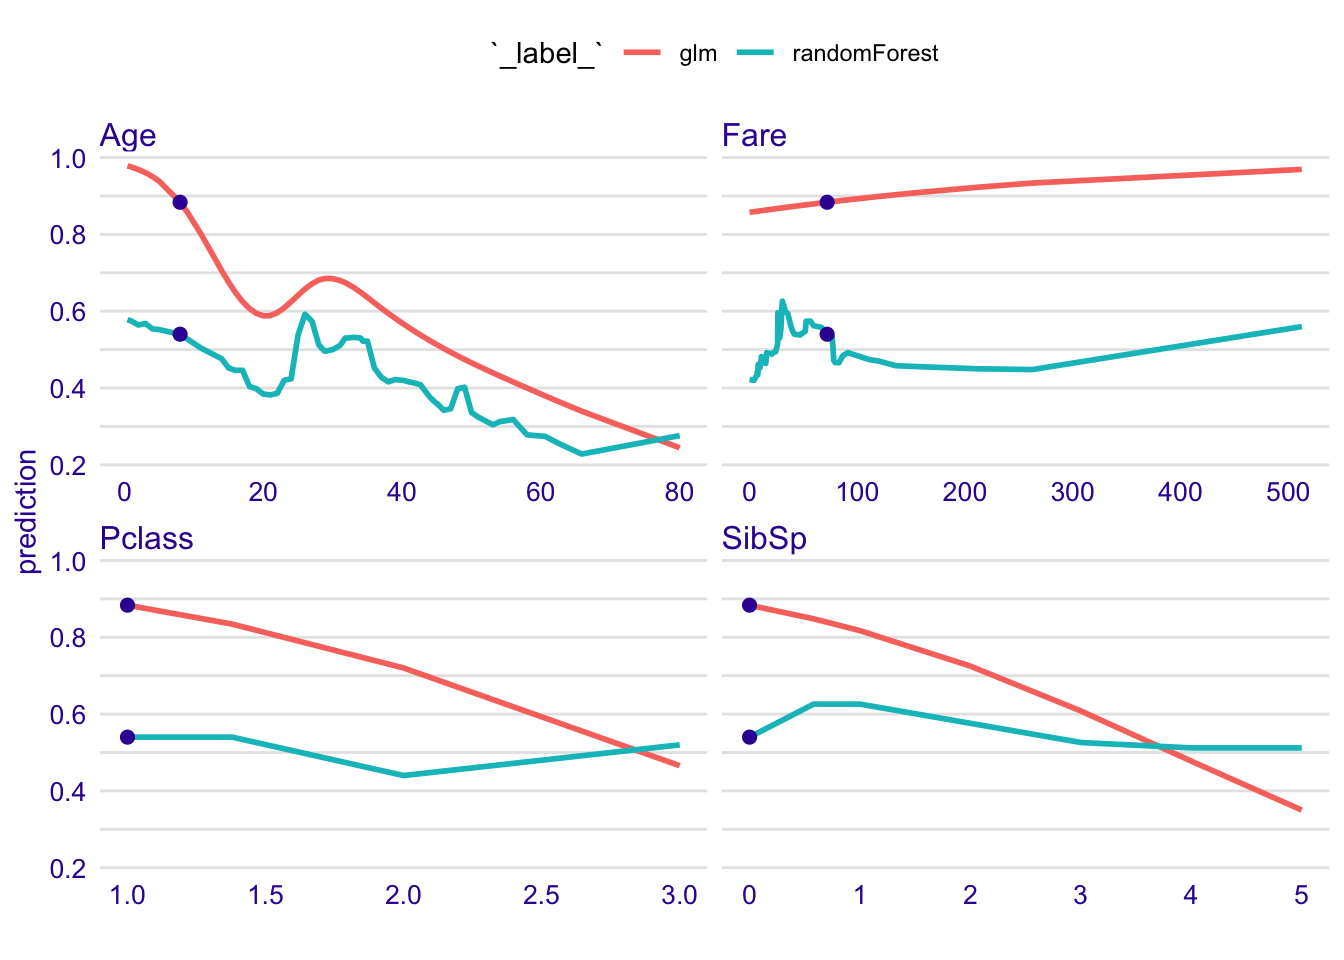
\includegraphics{PM_VEE_files/figure-latex/unnamed-chunk-25-1.pdf}

\hypertarget{the-iml-package}{%
\subsection{\texorpdfstring{\textbf{The iml
package}}{The iml package}}\label{the-iml-package}}

\begin{Shaded}
\begin{Highlighting}[]
\KeywordTok{library}\NormalTok{(}\StringTok{"iml"}\NormalTok{)}

\NormalTok{explainer_rf =}\StringTok{ }\NormalTok{Predictor}\OperatorTok{$}\KeywordTok{new}\NormalTok{(rf_model, }\DataTypeTok{data =}\NormalTok{ HR[,}\DecValTok{1}\OperatorTok{:}\DecValTok{5}\NormalTok{])}
\NormalTok{white_box =}\StringTok{ }\NormalTok{LocalModel}\OperatorTok{$}\KeywordTok{new}\NormalTok{(explainer_rf, }\DataTypeTok{x.interest =}\NormalTok{ new_observation[,}\DecValTok{1}\OperatorTok{:}\DecValTok{5}\NormalTok{], }\DataTypeTok{k =} \DecValTok{5}\NormalTok{)}
\NormalTok{white_box}
\end{Highlighting}
\end{Shaded}

\begin{verbatim}
## Interpretation method:  LocalModel 
## 
## 
## Analysed predictor: 
## Prediction task: unknown 
## 
## 
## Analysed data:
## Sampling from data.frame with 7847 rows and 5 columns.
## 
## Head of results:
##           beta x.recoded      effect x.original     feature feature.value
## 1  0.053490278       1.0  0.05349028       male gender=male   gender=male
## 2  0.005541233      57.7  0.31972915       57.7         age      age=57.7
## 3 -0.090377419      42.3 -3.82296481       42.3       hours    hours=42.3
## 4 -0.501469473       2.0 -1.00293895          2  evaluation  evaluation=2
## 5 -0.035232569       2.0 -0.07046514          2      salary      salary=2
## 6 -0.015995858       1.0 -0.01599586       male gender=male   gender=male
##   .class
## 1  fired
## 2  fired
## 3  fired
## 4  fired
## 5  fired
## 6     ok
\end{verbatim}

\begin{Shaded}
\begin{Highlighting}[]
\KeywordTok{plot}\NormalTok{(white_box)}
\end{Highlighting}
\end{Shaded}

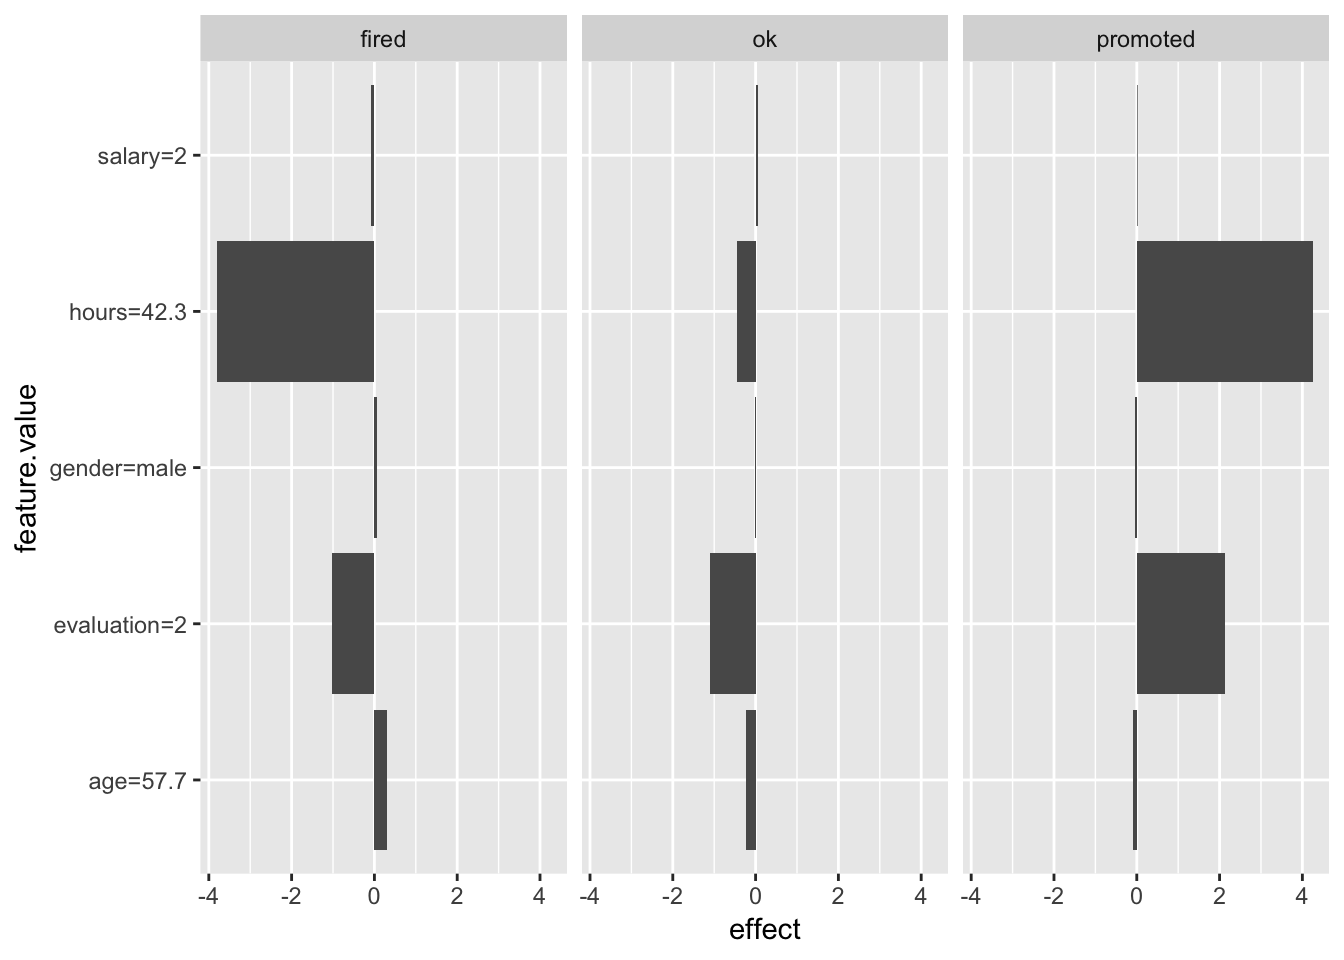
\includegraphics{PM_VEE_files/figure-latex/unnamed-chunk-26-1.pdf}

\hypertarget{ceterisParibus}{%
\chapter{Ceteris Paribus Principle}\label{ceterisParibus}}

In this section we introduce tools based on Ceteris Paribus principle.
The main goal for these tools is to help understand how changes in model
input affect changes in model output.

Presented explainers are linked with the second law introduced in
Section \ref{three-single-laws}, i.e.~law for prediction's speculations.
This is why these explainers are also known as \emph{What-If model
analysis} or \emph{Individual Conditional EXpectations} \citep{ICEbox}.
It turns out that it is easier to understand how blacx-box model is
working if we can play with it by changing variable by variable.

Think of following usecases:

\begin{itemize}
\tightlist
\item
  Think about a model for hart attack. How the model response would
  change if a patient cuts the number of smoked cigarettes by half or
  increase physical activity.
\item
  Think about a model for credit scoring. A customer gets a low score
  and is asking what he needs to change to increase this score to a
  certain level, to pass the bank criteria.
\item
  Think about a model for apartment prices. An investor wants to know
  how much the price may increase if apartment standard is upgraded.
\end{itemize}

\hypertarget{introduction-1}{%
\section{Introduction}\label{introduction-1}}

\emph{Ceteris paribus} is a Latin phrase meaning ``other things held
constant'' or ``all else unchanged''. Using this principle we examine
input variable per variable separatly, asumming that effects of all
other variables are unchanged. See Figure
\ref{fig:modelResponseCurveLine}

\begin{figure}

{\centering 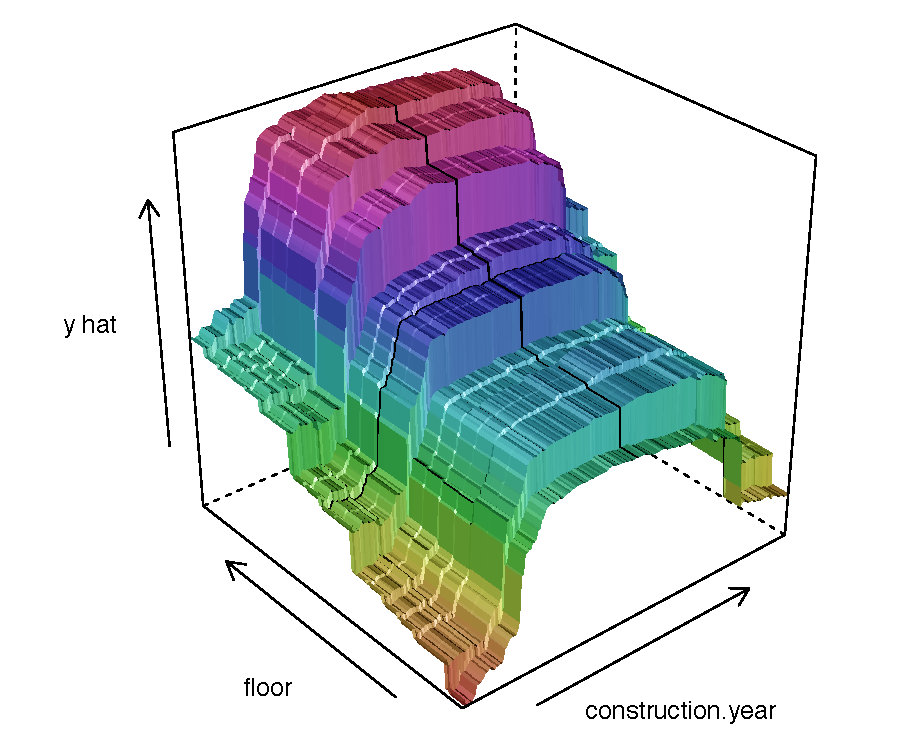
\includegraphics[width=0.7\linewidth]{figure/model_response_line} 

}

\caption{(fig:modelResponseCurveLine) A) Model response surface. Ceteris Paribus profiles marked with black curves helps to understand the curvature of the model response by updating only a single variable. B) CP profiles are individual conditional model responses}\label{fig:modelResponseCurveLine}
\end{figure}

Similar to the LIME method introduced in the section \ref{LIME}, Ceteris
Paribus profiles examine curvature of a model response function. The
difference between these two methods that LIME approximates the model
curvature with a simpler white-box model that is easier to present.
Usually the LIME model is sparse, thus our attention may be limited to
smaller number of dimensions. In contrary, the CP plots show conditional
model response for every variable. In the last subsection we discuss
pros and cons of this approach.

\hypertarget{ceterisParibus1d}{%
\section{1D profiles}\label{ceterisParibus1d}}

Let \(f_{M}(x): \mathcal R^{d} \rightarrow \mathcal R\) denote a
predictive model, i.e.~function that takes \(d\) dimensional vector and
calculate numerical score. Symbol \(x \in \mathcal R^d\) refers to a
point in the feature space. We use subscript \(x_i\) to refer to a
different data points and superscript \(x^j\) to refer to specific
dimensions. Additionally, let \(x^{-j}\) denote all coordinates except
\(j\)-th and let \(x|^j=z\) denote a data point \(x^*\) with all
coordinates equal to \(x\) except coordinate \(j\) equal to value \(z\).
I.e. \(\forall_{i \neq {j}} x^i = x^{*,i}\) and \(x^j = z\). In other
words \(x|^j=z\) denote a \(x\) with \(j\)th coordinate changed to
\(z\).

Now we can define uni-dimensional Ceteris Paribus Profile for model
\(f\), variable \(j\) and point \(x\) as

\[
CP^{f, j, x}(z) := f(x|^j = z).
\] I.e. CP profile is a model response obtained for observations created
based on \(x\) with coordinate \(j\) changed and all other coordinates
kept unchanged.

A natural way to visualise CP profiles is to use a profile plot as in
Figure \ref{fig:HRCPFiredHours}.

Figure \ref{fig:HRCPFiredHours} shows an example of Ceteris Paribus
profile. The black dot stands for prediction for a single observation.
Grey line show how the model response would change if in this single
observation coordinate \texttt{hours} will be changed to selected value.
One thing that we can read is that the model response is not smooth and
there is some variability along the profile. Second thing is that for
this particular observation the model response would drop significantly
if the variable \texttt{hours} will be higher than 45.

\begin{figure}

{\centering 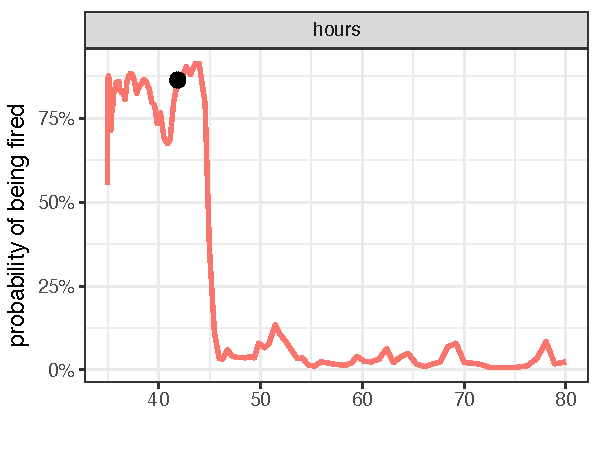
\includegraphics[width=0.5\linewidth]{figure/HR_cp_fired_hours} 

}

\caption{(fig:HRCPHiredHours) Ceteris Paribus profile for Random Forest model that assess the probability of being fired in call center as a function of average number of working hours}\label{fig:HRCPFiredHours}
\end{figure}

Since in the example dataset we are struggling with model for three
classes, one can plot CP profiles for each class in the same panel. See
an example in the Figure \ref{fig:HRCPAllHours}.

\begin{figure}

{\centering 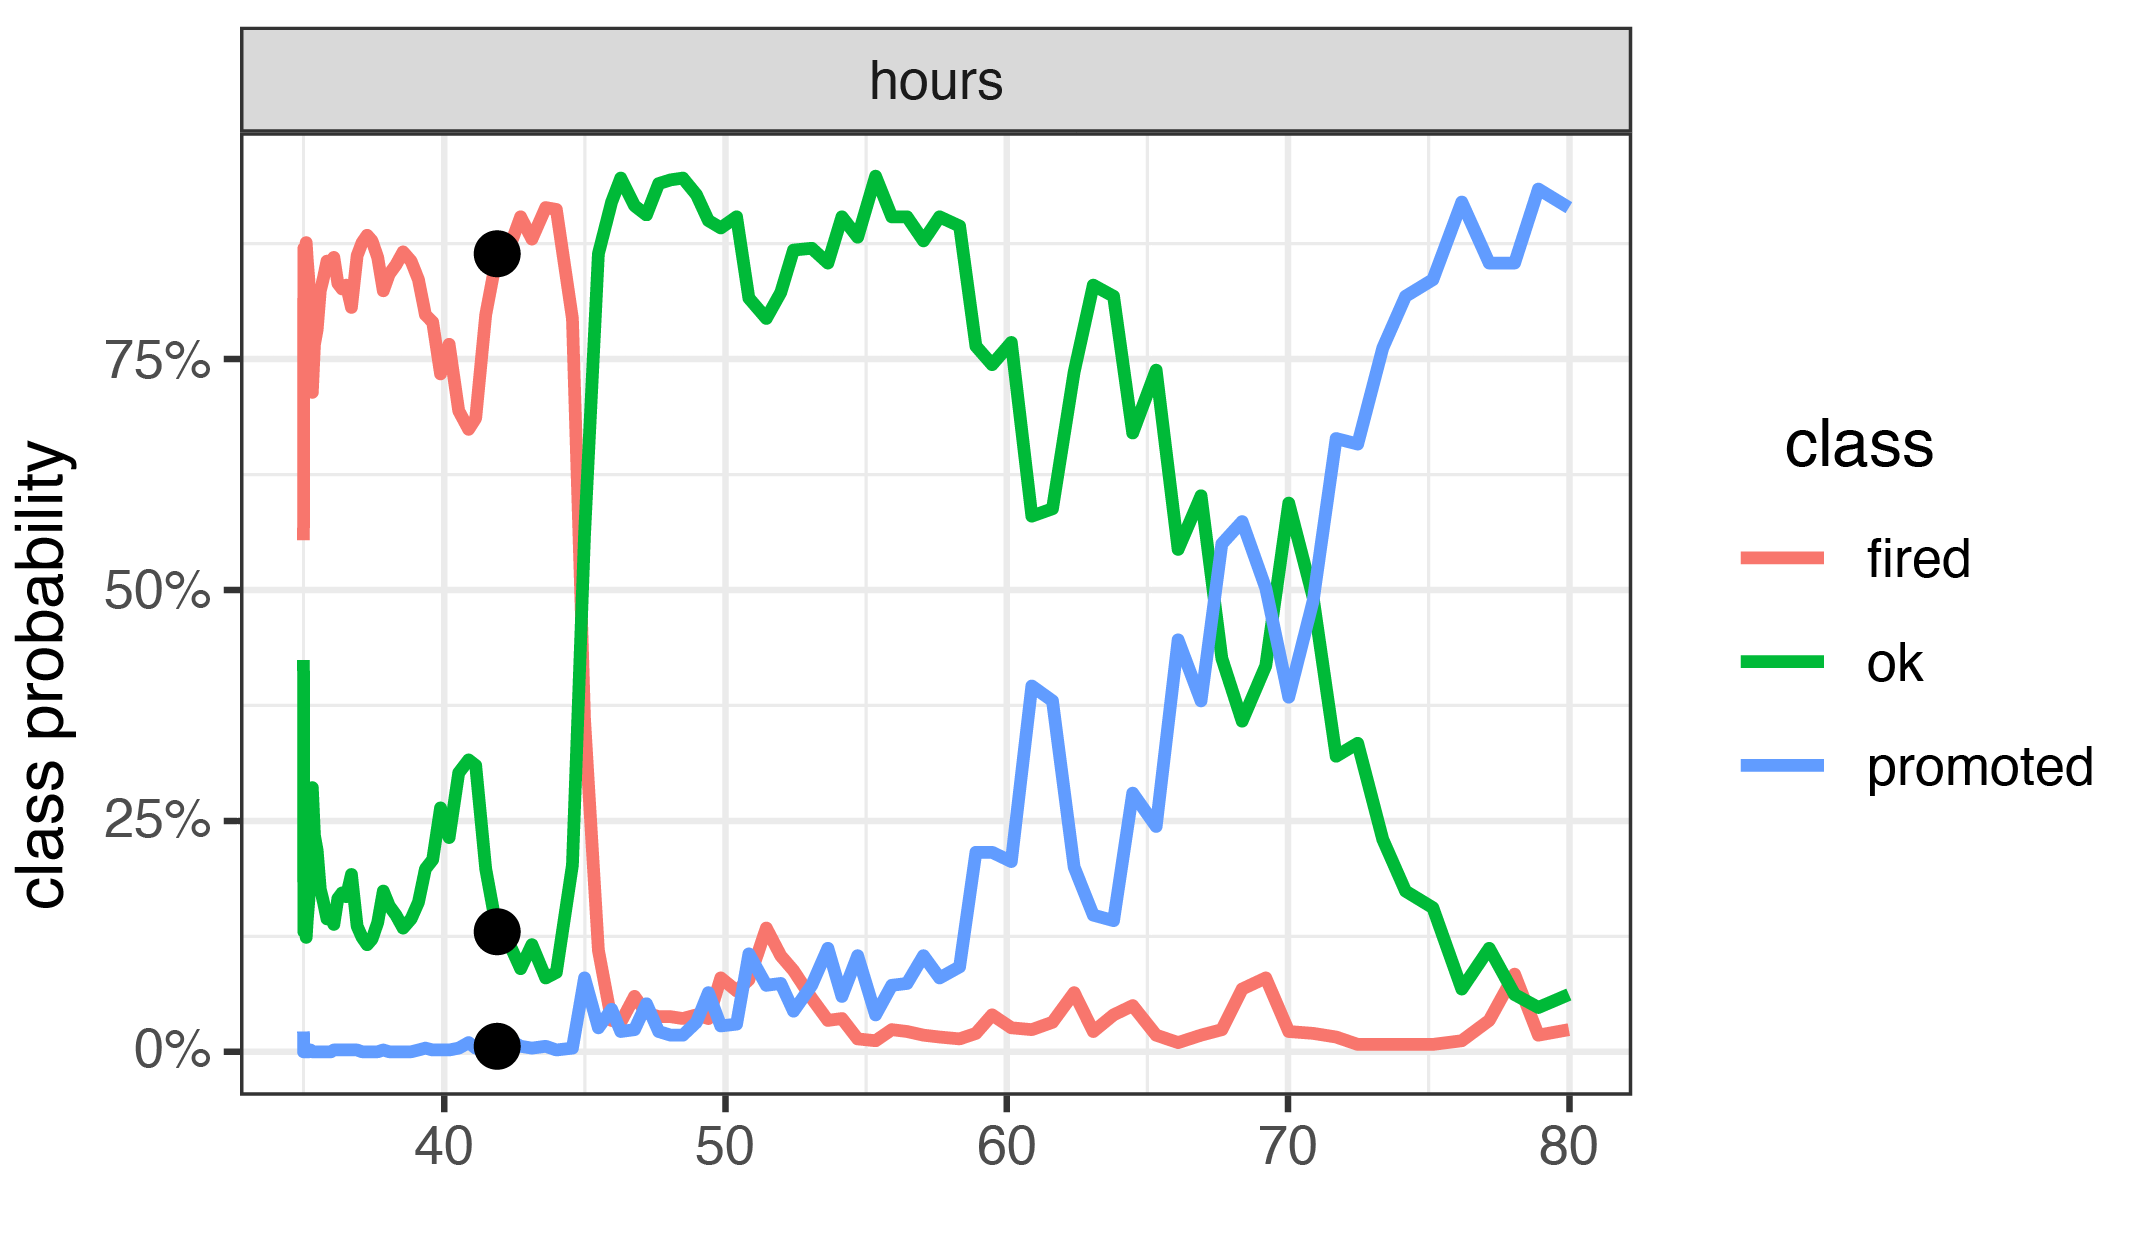
\includegraphics[width=0.6\linewidth]{figure/HR_cp_all_hours} 

}

\caption{(fig:HRCPAllHours) Ceteris Paribus profiles for three classess predicted by the Random Forest model as a function of average number of working hours}\label{fig:HRCPAllHours}
\end{figure}

Usually model input consist many variables, then it is beneficial to
show more variables at the same time. The easiest way to do so is to
plot consecutive variables on separate panels. See an example in Figure
\ref{fig:HRCPFiredAll}.

\begin{figure}

{\centering 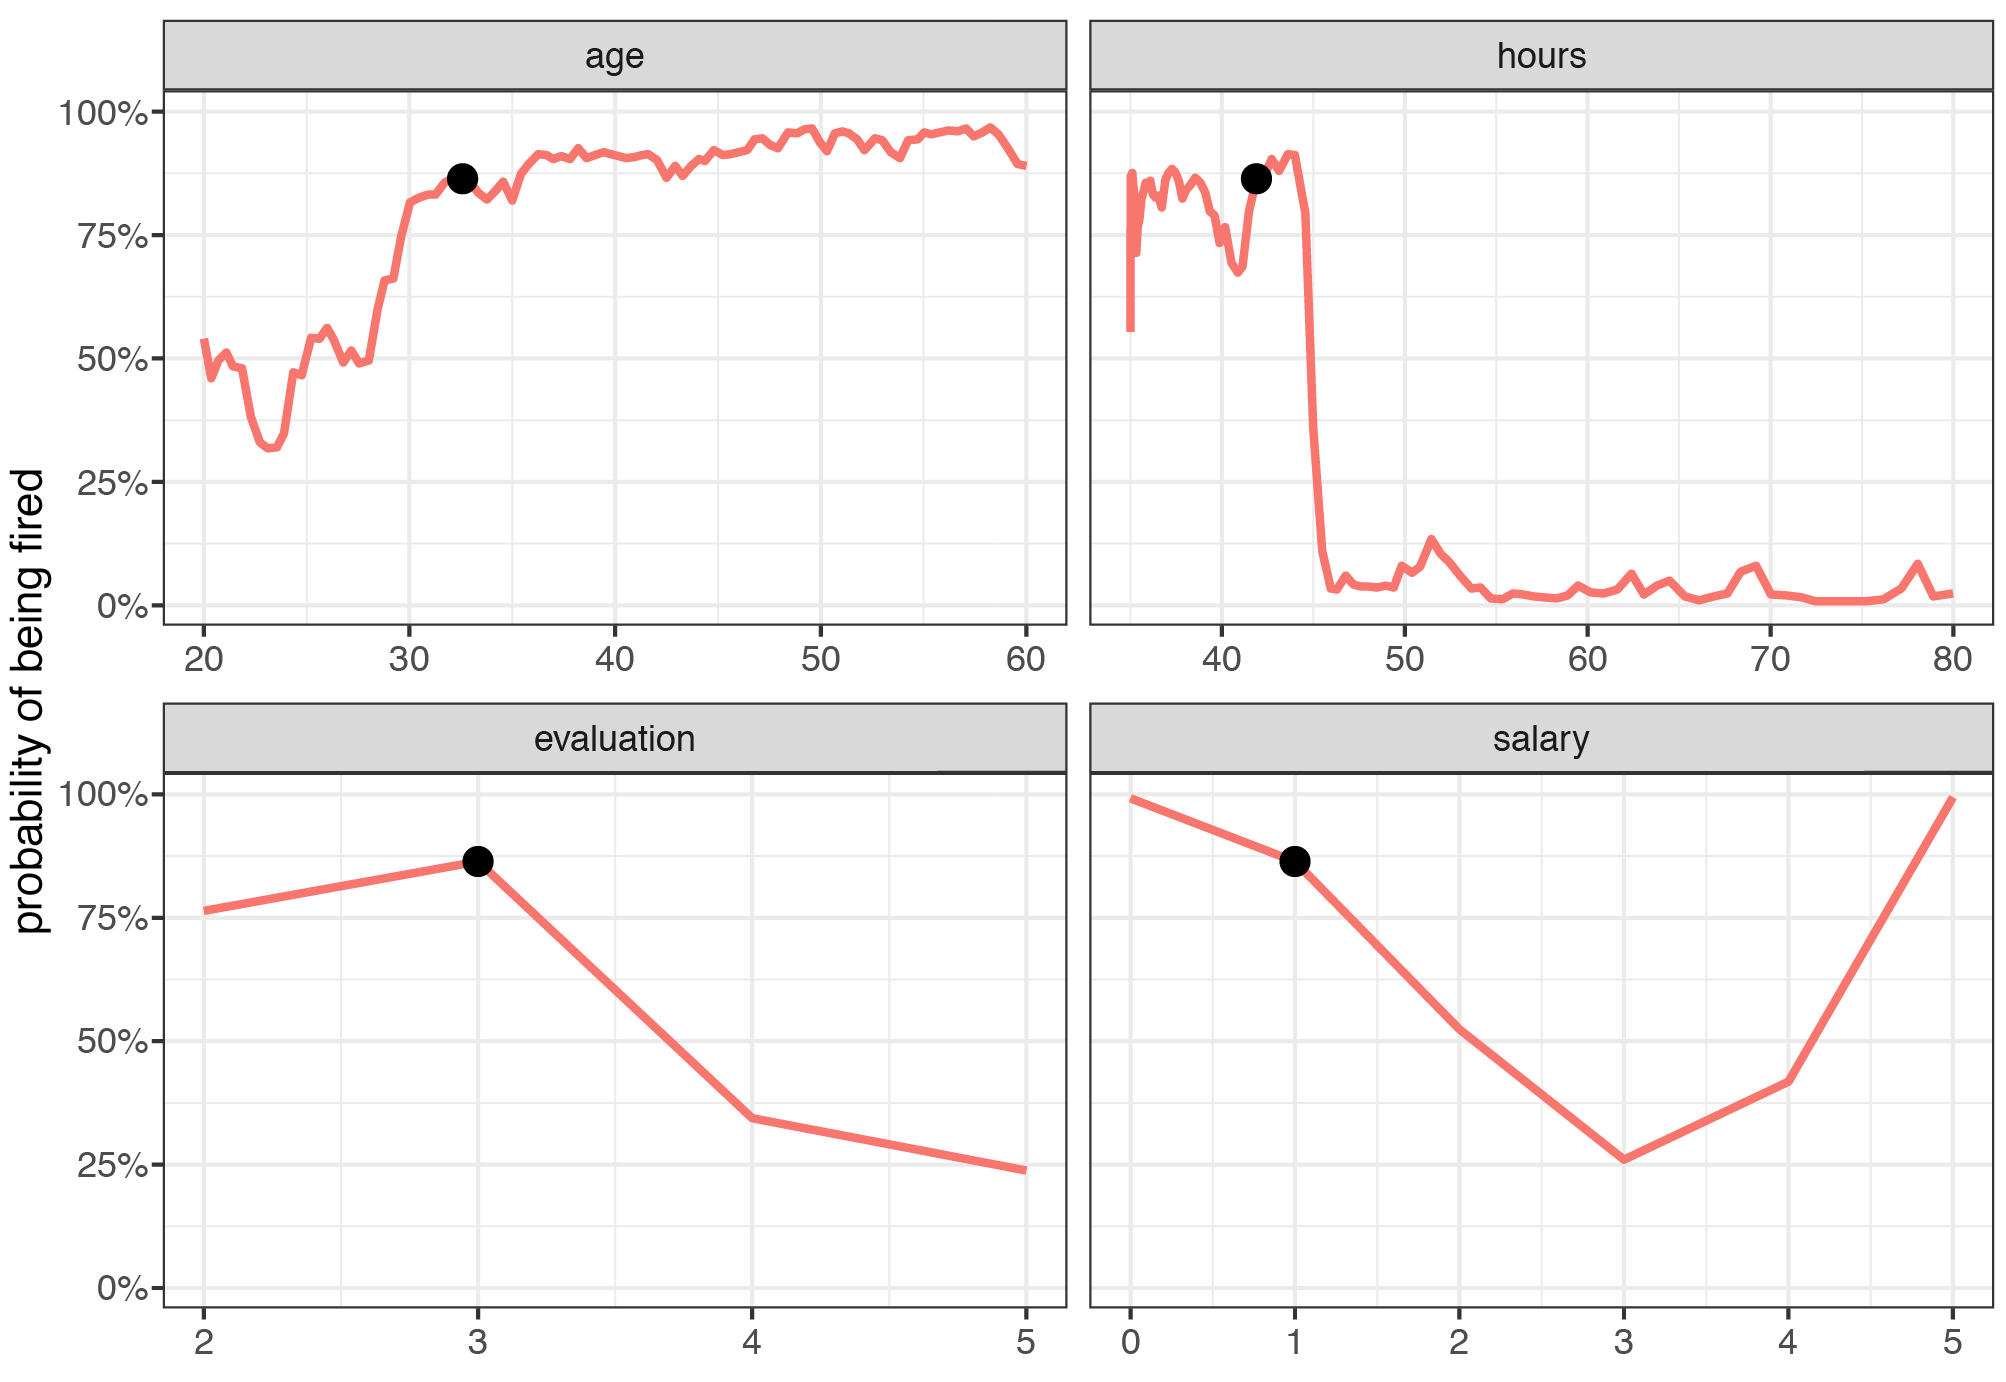
\includegraphics[width=0.7\linewidth]{figure/HR_cp_fired_all} 

}

\caption{(fig:HRCPFiredAll) Ceteris Paribus profiles for all continuous variables}\label{fig:HRCPFiredAll}
\end{figure}

\hypertarget{oscillations}{%
\section{Profile oscillations}\label{oscillations}}

Visual examination of variables is insightful, but for large number of
variables we end up with large number of panels, most of which are flat.
This is why we want to asses variable importance and show only profiles
for important variables. The advantage of CP profiles is that they lead
to a very natural and intuitive way of assessing the variable importance
for a single prediction. The intuition is: the more important variable
the larger are changes along the CP profile. If variable is not
important then model response will barely change. If variable is
important the CP profile change a lot for different values of a
variable.

Let's write it down in a more formal way.

Let \(vip^{CP}_j(x)\) denotes variable importance calculated based on CP
profiles in point \(x\) for variable \(j\).

\[
vip^{CP}_j(x) = \int_{-\inf}^{inf} |CP^{f,j,x}(z) - f(x)| dz
\]

So it's an absolute deviation from \(f(x)\). Note that one can consider
different modification of this coefficient:

\begin{enumerate}
\def\labelenumi{\arabic{enumi}.}
\tightlist
\item
  Deviations can be calculated not as a distance from \(f(x)\) but from
  average \(\bar CP^{f,j,x}(z)\).
\item
  The integral may be weighted based on the density of variable \(x^j\).
\item
  Instead of absolute deviations one may use root from average squares.
\end{enumerate}

TODO: we need to verify which approach is better. Anna Kozak is working
on this

The straightforward estimator for \(vip^{CP}_j(x)\) is

\[
\widehat{ vip^{CP}_j(x)} = \frac 1n \sum_{i=1}^n |CP^{f,j,x}(x_i) - f(x)|.
\]

Figure \ref{fig:CPVIPprofiles} shows the idea behind measuring
oscillations. The larger the highlighted area the more important is the
variable.

\begin{figure}

{\centering 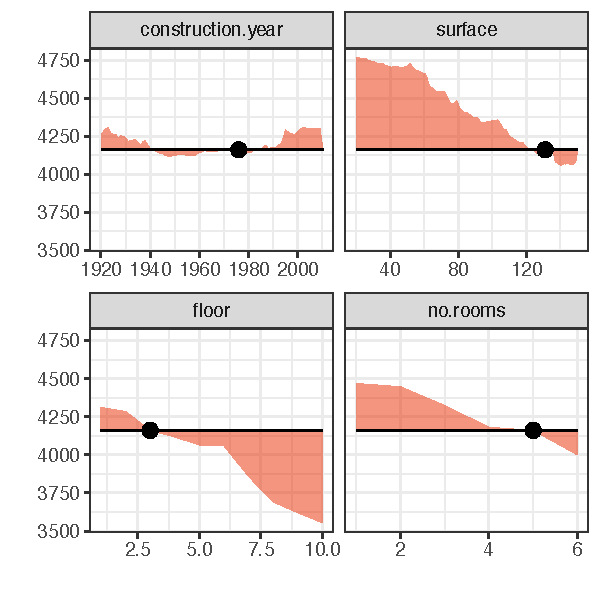
\includegraphics[width=0.5\linewidth]{figure/CP_VIP_profiles} 

}

\caption{(fig:CPVIPprofiles) CP oscillations are average deviations between CP profiles and the model response}\label{fig:CPVIPprofiles}
\end{figure}

Figure \ref{fig:CPVIP1} summarizes variable oscillations. Such visuals
help to quickly grasp how large are model oscillations around a specific
point.

\begin{figure}

{\centering 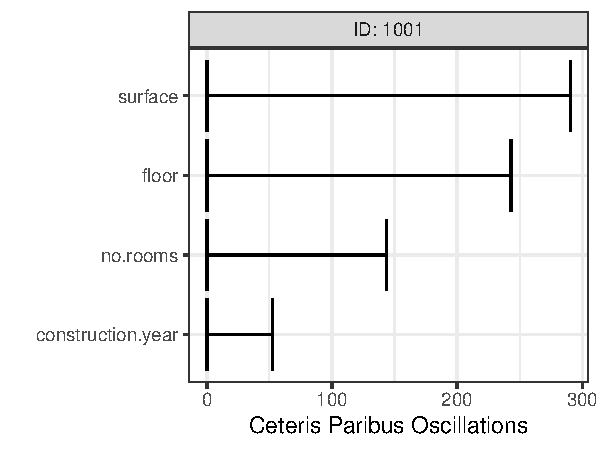
\includegraphics[width=0.4\linewidth]{figure/cp_vip_1} 

}

\caption{(fig:CPVIP1) Variable importance plots calculated for Ceteris Paribus profiles for observation ID: 1001}\label{fig:CPVIP1}
\end{figure}

\textbf{NOTE}

Variable importance for single prediction may be very different than
variable importance for the full model.

For example, consider a model \[
f(x_1, x_2) = x_1 * x_2
\] where variables \(x_1\) and \(x_2\) takes values in \([0,1]\).

From the global perspective both variables are equally important.

But local variable importance is very different. Around point
\(x = (0, 1)\) the importance of \(x_1\) is much larger than \(x_2\).
This is because profile for \(f(z, 1)\) have larger oscillations than
\(f(0, z)\).

\hypertarget{d-profiles}{%
\section{2D profiles}\label{d-profiles}}

The definition of ceteris paribus profiles given in section
\ref{ceterisParibus1d} may be easily extended to two and more variables.
Also definition of CP oscillations \ref{oscillations} have straight
forward generalization for larger number of dimensions. Such
generalisations are usefull when model is non additive. Presence of
pairwise interactions may be detected with 2D Ceteris Paribus plots.

Let's define two-dimensional Ceteris Paribus Profile for model \(f\),
variables \(j\) and \(k\) and point \(x\) as

\[
CP^{f, (j,k), x}(z_1, z_2) := f(x|^{(j,k)} = (z_1,z_2)).
\] I.e. CP profile is a model response obtained for observations created
based on \(x\) with \(j\) and \(k\) coordinates changed to
\((z_1, z_2)\) and all other coordinates kept unchanged.

A natural way to visualise 2D CP profiles is to use a level plot as in
Figure \ref{fig:CP2Dsurflor}.

\begin{figure}

{\centering 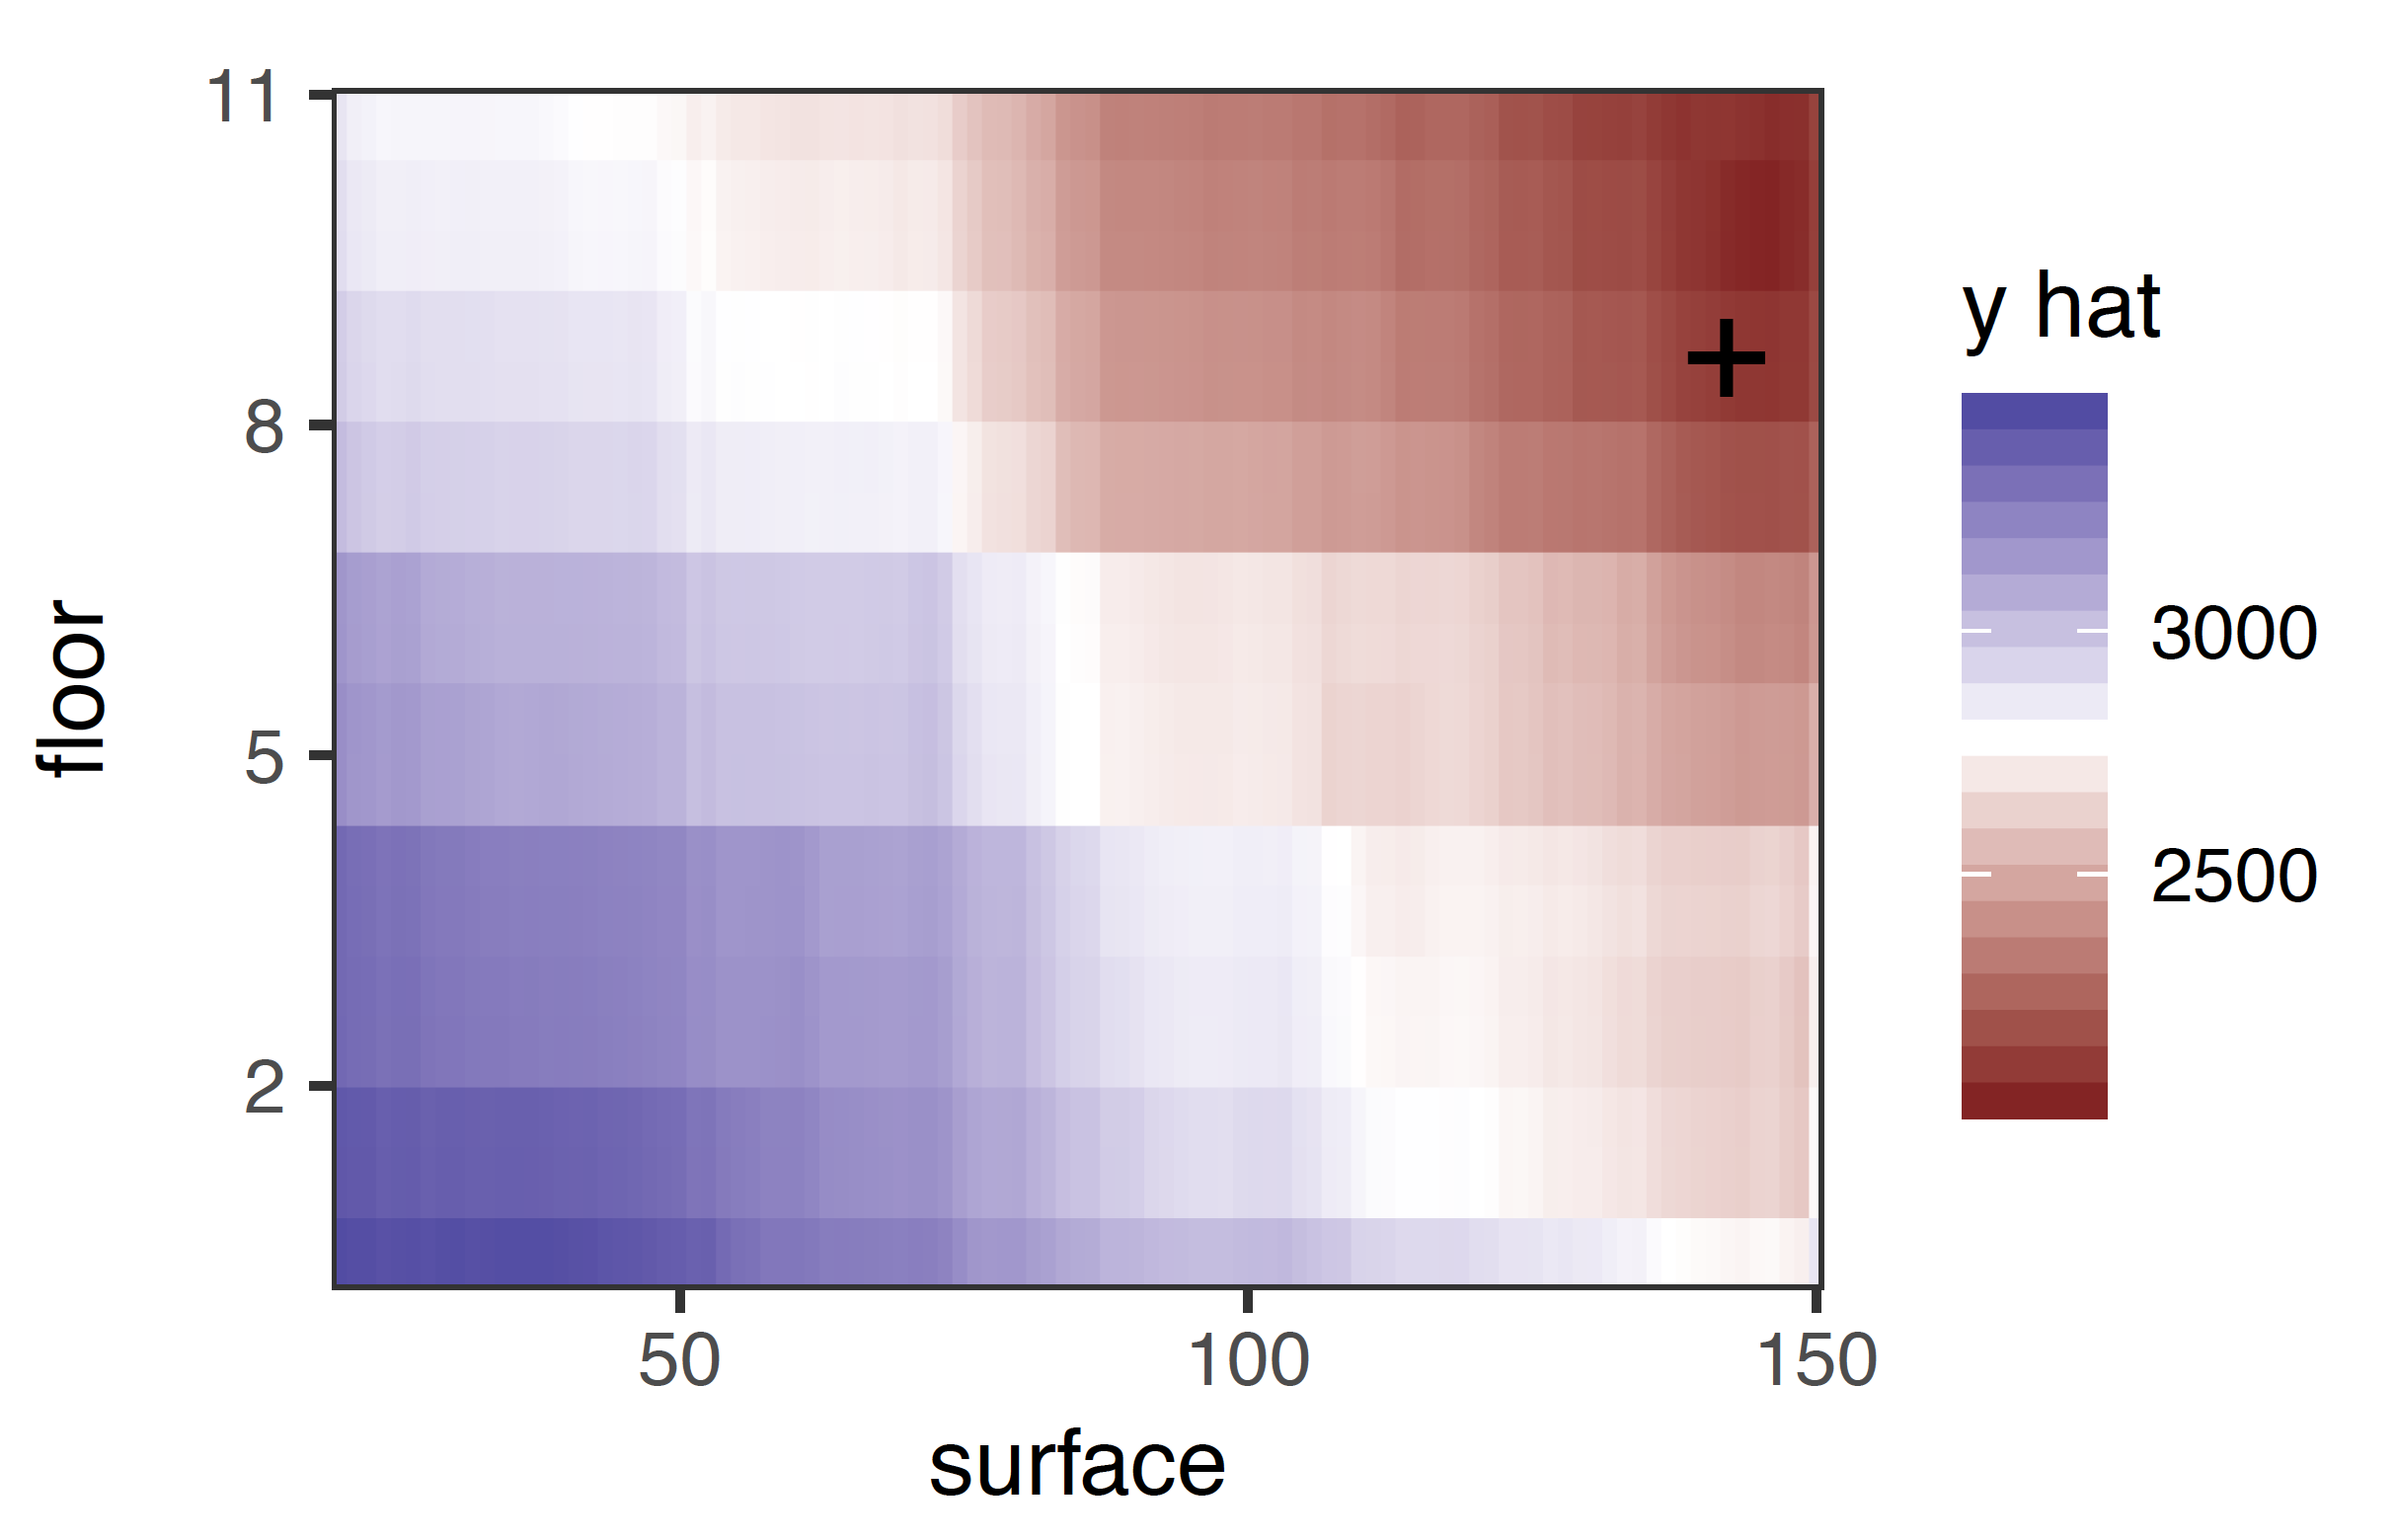
\includegraphics[width=0.6\linewidth]{figure/cp_2d_surf_floor} 

}

\caption{(fig:CP2Dsurflor) Ceteris Paribus plot for a pair of variales. Black cross marks coordinated for the observation of interest. Presented model estimates price of an appartment}\label{fig:CP2Dsurflor}
\end{figure}

If number of variables is small or moderate thein it is possible to
present all pairs of variables. See an example in Figure
\ref{fig:CP2Dall}.

\begin{figure}

{\centering 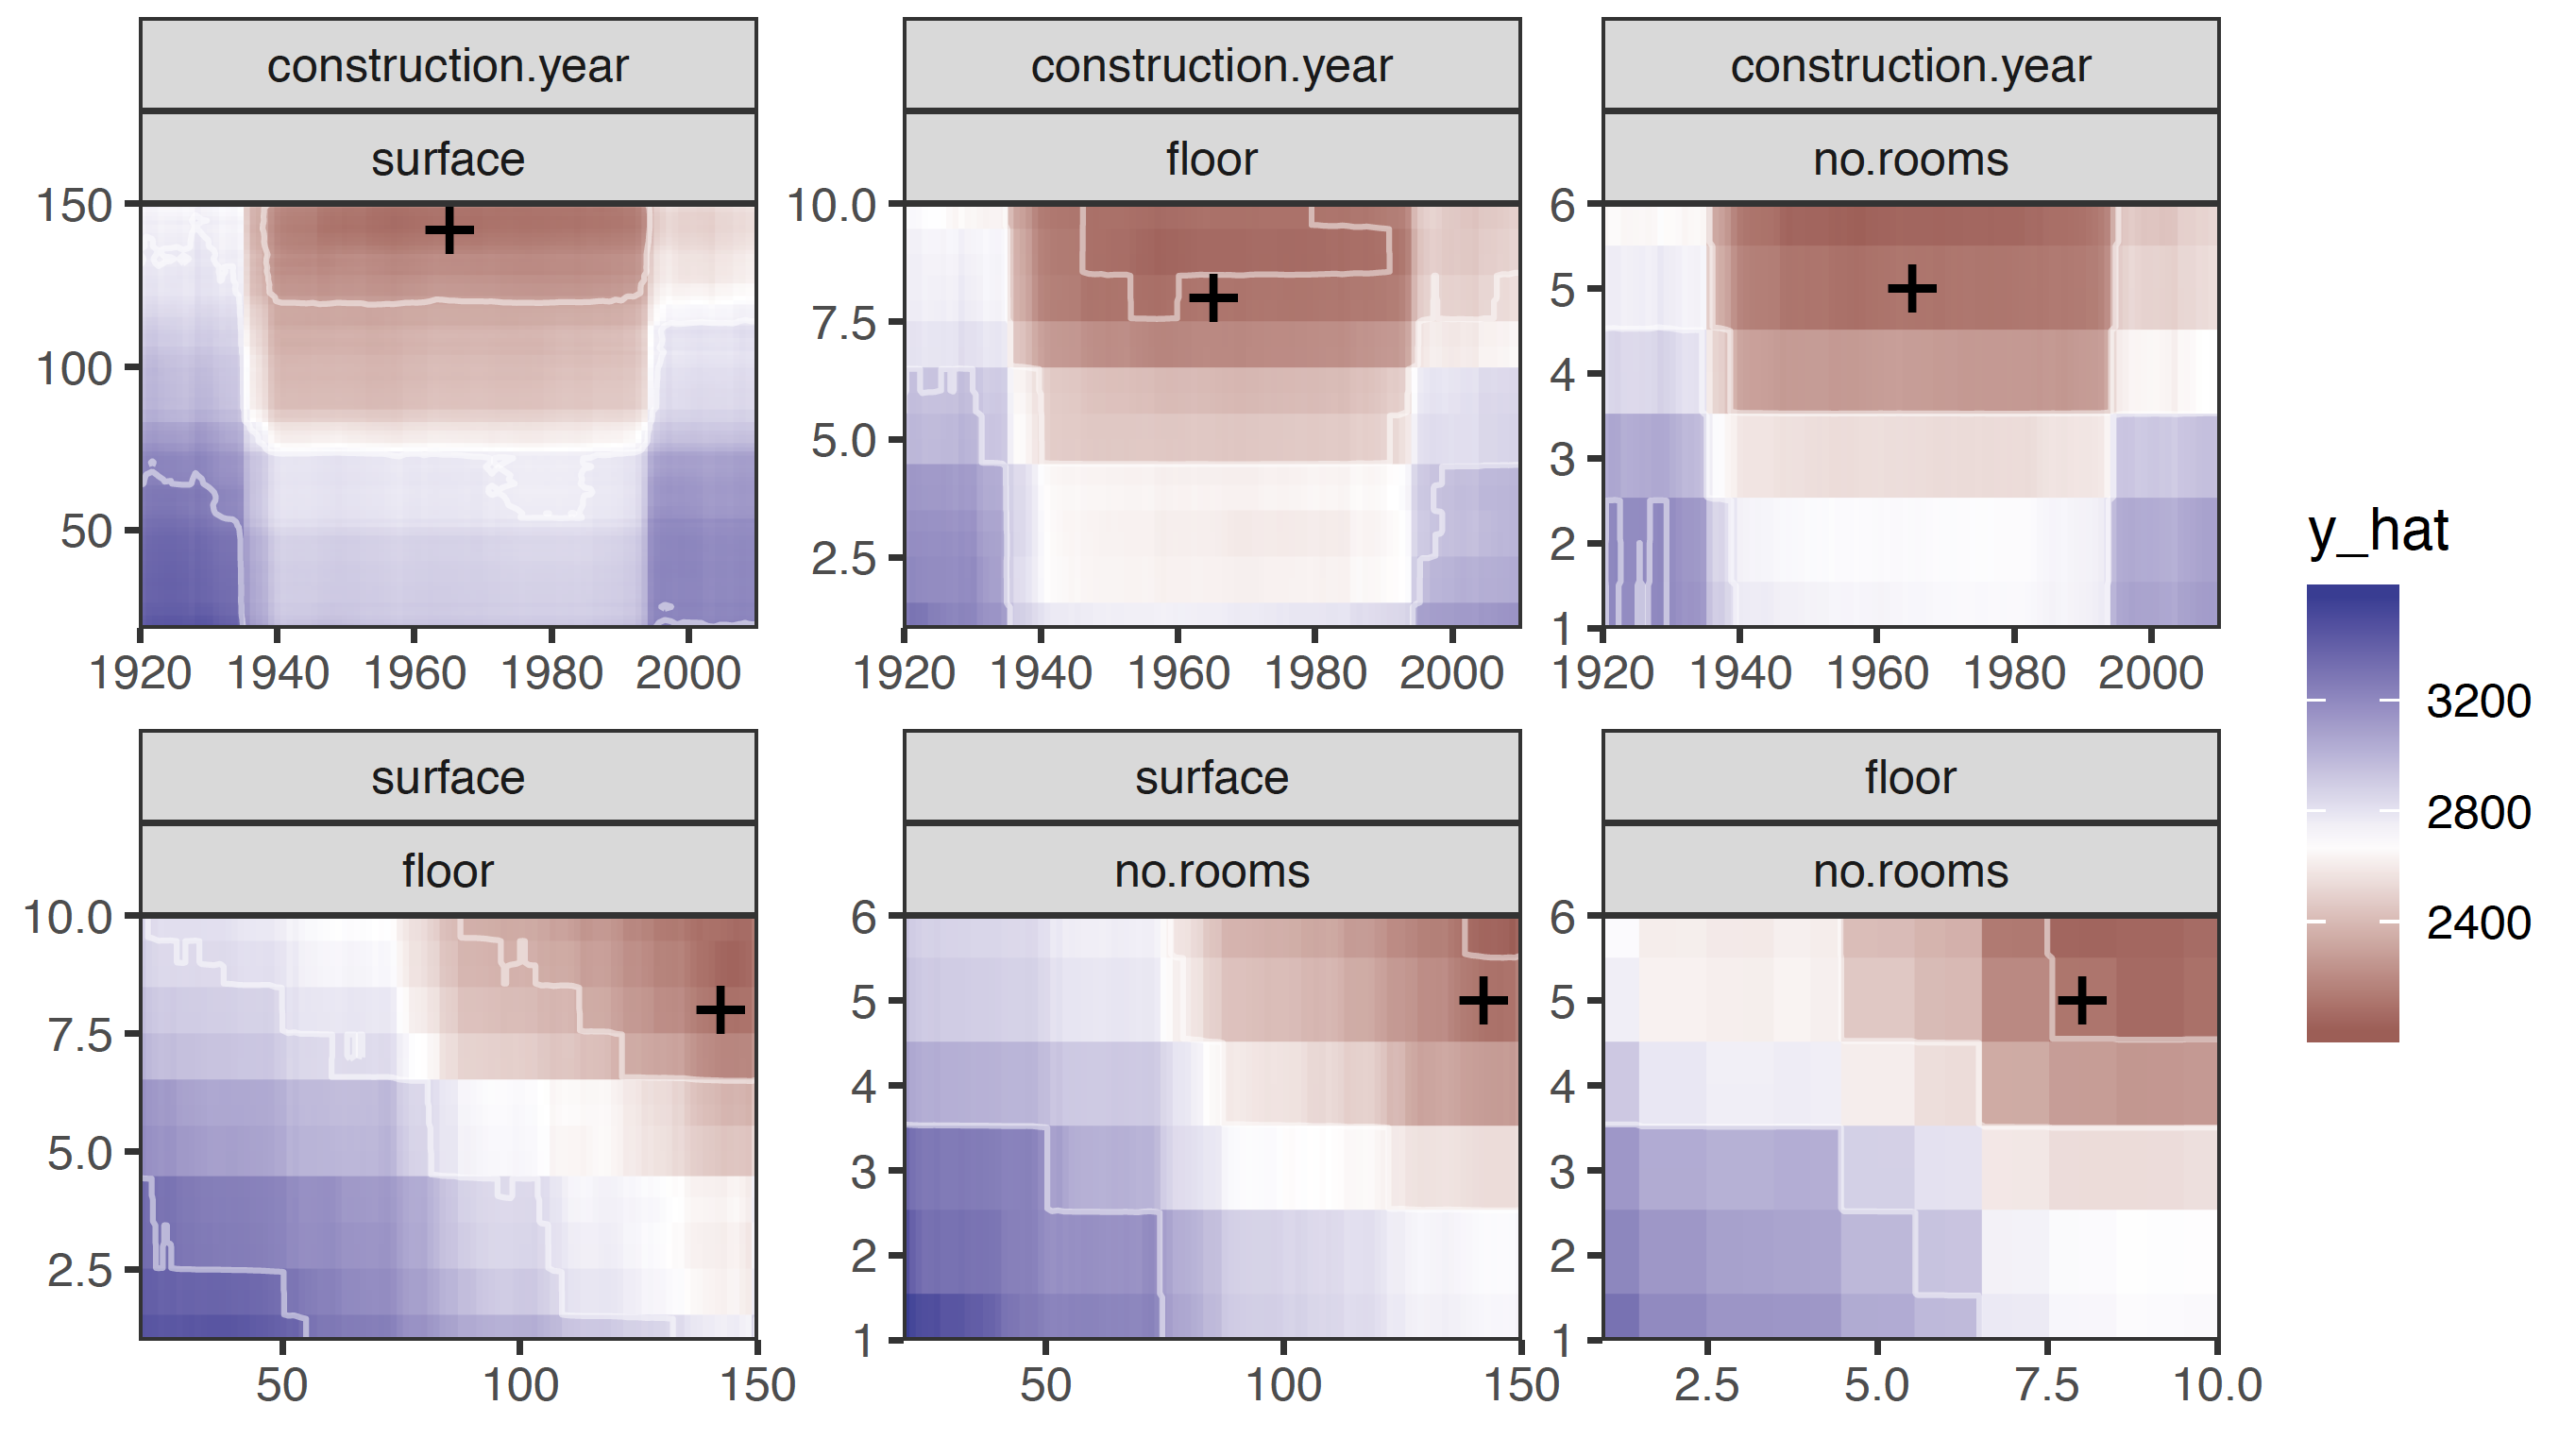
\includegraphics[width=0.9\linewidth]{figure/cp_2d_all} 

}

\caption{(fig:CP2Dall) Ceteris Paribus plot for all pairs of variales.}\label{fig:CP2Dall}
\end{figure}

\hypertarget{local-model-fidelity}{%
\section{Local model fidelity}\label{local-model-fidelity}}

Ceteris Paribus profiles are also a useful tool to validate local model
fidelity. It may happen that global performance of the model is good,
while for some points the local fit is very bad. Local fidelity helps to
understand how good is the model fit around point of interest.

How does it work?

The idea behind fidelity plots is to select some number of points from
the validation dataset that are closes to the point of interest. It's a
similar approach as in k nearest neighbours. Then for these neighbours
we may plot Ceteris Paribus Profiles and check how stable they are.

Also, if we know true taget values for points from the validation
dataset we may plot residuals to show how large are residuals.

An example fidelity plot is presented in Figure \ref{fig:CPfidelity1}.
Black line shows the CP profiles for the point of interest, while grey
lines show CP profiles for neihgbors. Red intervals stand for residuals
and in this example it looks like residuals for neighbours are all
negative. Thus maybe model is biased around the point of interest.

\begin{figure}

{\centering 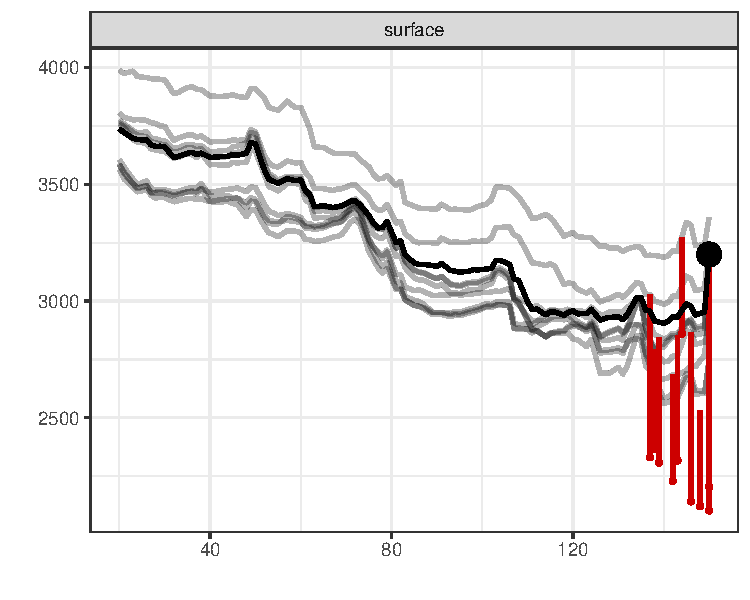
\includegraphics[width=0.7\linewidth]{figure/cp_fidelity_1} 

}

\caption{(fig:CPfidelity1) Local fidelity plots. Black line shows the CP profile for the point of interest. Grey lines show CP profiles for nearest neighbors. Red intervals correspond to residuals. Each red interval starts in a model prediction for a selected neighbor and ends in its true value of target variable.}\label{fig:CPfidelity1}
\end{figure}

This observation may be confirmed by plots that compare distribution of
all residuals against distribution of residuals for neighbors.

See Figure \ref{CPfidelityBoxplot} for an example. Here residuals for
neighbors are shifted towards highest values. This suggests that the
model response is biased around the observation of interest.

\begin{figure}

{\centering 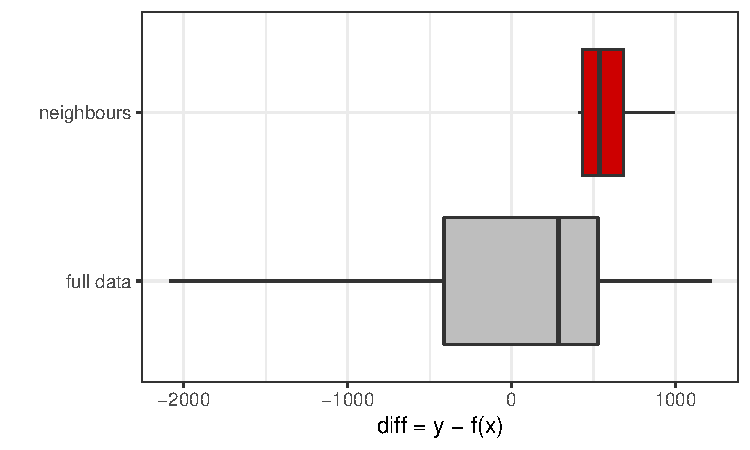
\includegraphics[width=0.7\linewidth]{figure/cp_fidelity_boxplot} 

}

\caption{(fig:CPfidelityBoxplot) Distribution of residuals for whole validation data (grey boxplot) and for selected closes 15 neighbors (red boxplot).}\label{fig:CPfidelityBoxplot}
\end{figure}

\hypertarget{pros-and-cons-4}{%
\section{Pros and cons}\label{pros-and-cons-4}}

Ceteris Paribus principle gives a uniform and extendable approach to
model exploration. Below we summarize key strengths and weaknesses of
this approach.

\textbf{Pros}

\begin{itemize}
\tightlist
\item
  Graphical representation of Ceteris Paribus profile is easy to
  understand.
\item
  Ceteris Paribus profiles are compact and it is easy to fit many models
  or many variables in a small space.
\item
  Ceteris Paribus profiles helps to understand how model response would
  change and how stable it is
\item
  Oscillations calculated for CP profiles helps to select the most
  important variables.
\item
  2D Ceteris Paribus profiles help to identify pairwise interactions
  between variables.
\end{itemize}

\textbf{Cons}

\begin{itemize}
\tightlist
\item
  If variables are correlated (like surface and number of rooms) then
  the `\emph{everything else kept unchanged}' approach leads to
  unrealistic settings.
\item
  Interactions between variables are not visible in 1D plots.
\item
  This tool is not suited for very wide data, like hundreds or thousands
  of variables.
\item
  Visualization of categorical variables is non trivial.
\end{itemize}

\hypertarget{code-snippets-for-r-4}{%
\section{Code snippets for R}\label{code-snippets-for-r-4}}

In this section we present key features of the \texttt{ceterisParibus}
package for R \citep{R-ceterisParibus}. This package covers all features
presented in this chapter. It is available on CRAN and GitHub. Find more
examples at the website of this package
\texttt{https://pbiecek.github.io/ceterisParibus/}.

\textbf{Model preparation}

In this section we will present examples based on the
\texttt{apartments} dataset. See section TODO for more details.

\begin{Shaded}
\begin{Highlighting}[]
\KeywordTok{library}\NormalTok{(}\StringTok{"DALEX"}\NormalTok{)}
\KeywordTok{head}\NormalTok{(apartments)}
\end{Highlighting}
\end{Shaded}

\begin{verbatim}
##   m2.price construction.year surface floor no.rooms    district
## 1     5897              1953      25     3        1 Srodmiescie
## 2     1818              1992     143     9        5     Bielany
## 3     3643              1937      56     1        2       Praga
## 4     3517              1995      93     7        3      Ochota
## 5     3013              1992     144     6        5     Mokotow
## 6     5795              1926      61     6        2 Srodmiescie
\end{verbatim}

The problem here is to predict average price for square meter for an
apartment. Let's build a random forest model with \texttt{randomForest}
package \citep{R-randomForest}.

\begin{Shaded}
\begin{Highlighting}[]
\KeywordTok{library}\NormalTok{(}\StringTok{"randomForest"}\NormalTok{)}
\NormalTok{rf_model <-}\StringTok{ }\KeywordTok{randomForest}\NormalTok{(m2.price }\OperatorTok{~}\StringTok{ }\NormalTok{construction.year }\OperatorTok{+}\StringTok{ }\NormalTok{surface }\OperatorTok{+}\StringTok{ }\NormalTok{floor }\OperatorTok{+}
\StringTok{      }\NormalTok{no.rooms, }\DataTypeTok{data =}\NormalTok{ apartments)}
\NormalTok{rf_model}
\end{Highlighting}
\end{Shaded}

\begin{verbatim}
## 
## Call:
##  randomForest(formula = m2.price ~ construction.year + surface +      floor + no.rooms, data = apartments) 
##                Type of random forest: regression
##                      Number of trees: 500
## No. of variables tried at each split: 1
## 
##           Mean of squared residuals: 486368.4
##                     % Var explained: 40.78
\end{verbatim}

Model exploration with \texttt{ceterisParibus} package is performed in
four steps.

\textbf{1. Create an explainer - wrapper around model and validation
data.}

Since all other functions work in a model agnostic fashion, first we
need to define a wrapper around the model. Here we are using the
\texttt{explain()} function from \texttt{DALEX} package \citep{R-DALEX}.

\begin{Shaded}
\begin{Highlighting}[]
\KeywordTok{library}\NormalTok{(}\StringTok{"DALEX"}\NormalTok{)}
\NormalTok{explainer_rf <-}\StringTok{ }\KeywordTok{explain}\NormalTok{(rf_model,}
      \DataTypeTok{data =}\NormalTok{ apartmentsTest, }\DataTypeTok{y =}\NormalTok{ apartmentsTest}\OperatorTok{$}\NormalTok{m2.price)}
\NormalTok{explainer_rf}
\end{Highlighting}
\end{Shaded}

\begin{verbatim}
## Model label:  randomForest 
## Model class:  randomForest.formula,randomForest 
## Data head  :
##      m2.price construction.year surface floor no.rooms    district
## 1001     4644              1976     131     3        5 Srodmiescie
## 1002     3082              1978     112     9        4     Mokotow
\end{verbatim}

\textbf{2. Define point of interest.}

Certeris Paribus profiles explore model around a single point.

\begin{Shaded}
\begin{Highlighting}[]
\NormalTok{new_apartment <-}\StringTok{ }\KeywordTok{data.frame}\NormalTok{(}\DataTypeTok{construction.year =} \DecValTok{1965}\NormalTok{, }\DataTypeTok{no.rooms =} \DecValTok{5}\NormalTok{, }\DataTypeTok{surface =} \DecValTok{142}\NormalTok{, }\DataTypeTok{floor =} \DecValTok{8}\NormalTok{)}
\NormalTok{new_apartment}
\end{Highlighting}
\end{Shaded}

\begin{verbatim}
##   construction.year no.rooms surface floor
## 1              1965        5     142     8
\end{verbatim}

\begin{Shaded}
\begin{Highlighting}[]
\KeywordTok{predict}\NormalTok{(rf_model, new_apartment)}
\end{Highlighting}
\end{Shaded}

\begin{verbatim}
##        1 
## 2309.995
\end{verbatim}

\textbf{3. Calculate CP profiles}

The \texttt{ceteris\_paribus()} function calculates CP profiles for
selected model around selected observation.

By default CP profiles are calculated for all numerical variables. Use
the \texttt{variables} argument to select subset of interesting
variables. The result from \texttt{ceteris\_paribus()}function is a data
frame with model predictions for modified points around the point of
interest.

\begin{Shaded}
\begin{Highlighting}[]
\KeywordTok{library}\NormalTok{(}\StringTok{"ceterisParibus"}\NormalTok{)}
\NormalTok{cp_rf <-}\StringTok{ }\KeywordTok{ceteris_paribus}\NormalTok{(explainer_rf, new_apartment, }
                            \DataTypeTok{variables =} \KeywordTok{c}\NormalTok{(}\StringTok{"construction.year"}\NormalTok{, }\StringTok{"floor"}\NormalTok{))}
\NormalTok{cp_rf}
\end{Highlighting}
\end{Shaded}

\begin{verbatim}
## Top profiles    : 
##     construction.year no.rooms surface floor   _yhat_           _vname_
## 1                1920        5     142     8 3080.774 construction.year
## 1.1              1921        5     142     8 3107.434 construction.year
## 1.2              1922        5     142     8 3101.698 construction.year
## 1.3              1923        5     142     8 3066.222 construction.year
## 1.4              1923        5     142     8 3066.222 construction.year
## 1.5              1924        5     142     8 3079.564 construction.year
##     _ids_      _label_
## 1       1 randomForest
## 1.1     1 randomForest
## 1.2     1 randomForest
## 1.3     1 randomForest
## 1.4     1 randomForest
## 1.5     1 randomForest
## 
## 
## Top observations:
##   construction.year no.rooms surface floor   _yhat_      _label_
## 1              1965        5     142     8 2309.995 randomForest
\end{verbatim}

\textbf{4. Plot CP profiles.}

Generic \texttt{plot()} function plot CP profiles. It returns a
\texttt{ggplot2} object that can be polished if needed. Use additional
arguments of this function to select colors and sizes for elements
visible in the plot.

\begin{Shaded}
\begin{Highlighting}[]
\KeywordTok{plot}\NormalTok{(cp_rf) }
\end{Highlighting}
\end{Shaded}

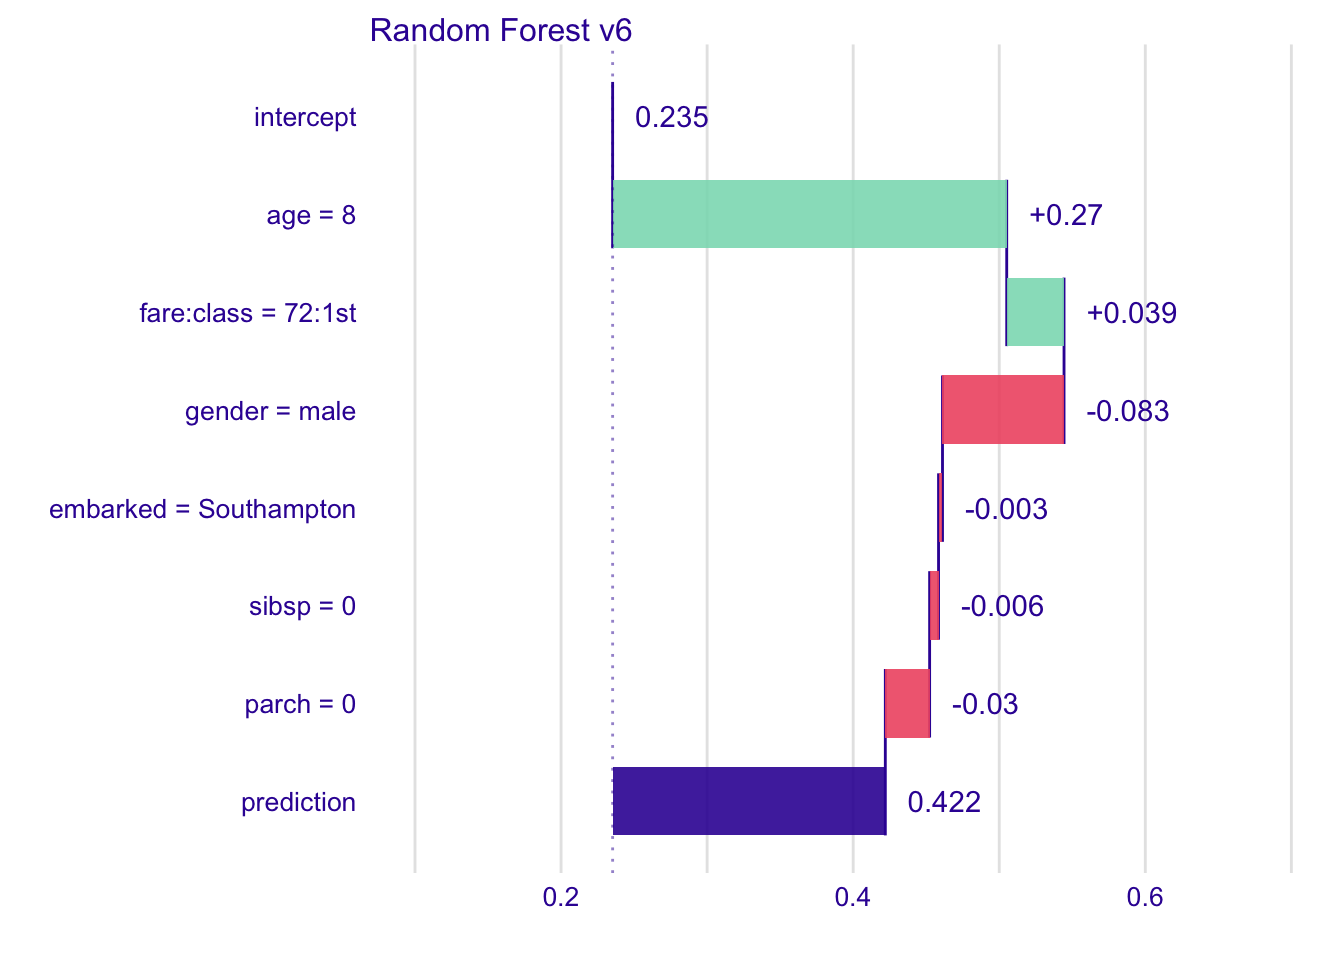
\includegraphics{PM_VEE_files/figure-latex/unnamed-chunk-32-1.pdf}

One of very useful features of \texttt{ceterisParibus} explainers is
that profiles for two or more models may be superimposed in a single
plot. This helps in model comparisons.

Let's create a linear model for this dataset and repeat steps 1-3 for
the lm model.

\begin{Shaded}
\begin{Highlighting}[]
\NormalTok{lm_model <-}\StringTok{ }\KeywordTok{lm}\NormalTok{(m2.price }\OperatorTok{~}\StringTok{ }\NormalTok{construction.year }\OperatorTok{+}\StringTok{ }\NormalTok{surface }\OperatorTok{+}\StringTok{ }\NormalTok{floor }\OperatorTok{+}
\StringTok{      }\NormalTok{no.rooms, }\DataTypeTok{data =}\NormalTok{ apartments)}
\NormalTok{explainer_lm <-}\StringTok{ }\KeywordTok{explain}\NormalTok{(lm_model,}
      \DataTypeTok{data =}\NormalTok{ apartmentsTest, }\DataTypeTok{y =}\NormalTok{ apartmentsTest}\OperatorTok{$}\NormalTok{m2.price)}
\NormalTok{cp_lm <-}\StringTok{ }\KeywordTok{ceteris_paribus}\NormalTok{(explainer_lm, new_apartment, }
                            \DataTypeTok{variables =} \KeywordTok{c}\NormalTok{(}\StringTok{"construction.year"}\NormalTok{, }\StringTok{"floor"}\NormalTok{))}
\end{Highlighting}
\end{Shaded}

Now we can use function \texttt{plot()} to compare both models in a
single chart. Additional argument \texttt{color\ =\ "\_label\_"} set
color as a key for model.

\begin{Shaded}
\begin{Highlighting}[]
\KeywordTok{plot}\NormalTok{(cp_rf, cp_lm, }\DataTypeTok{color =} \StringTok{"_label_"}\NormalTok{)}
\end{Highlighting}
\end{Shaded}

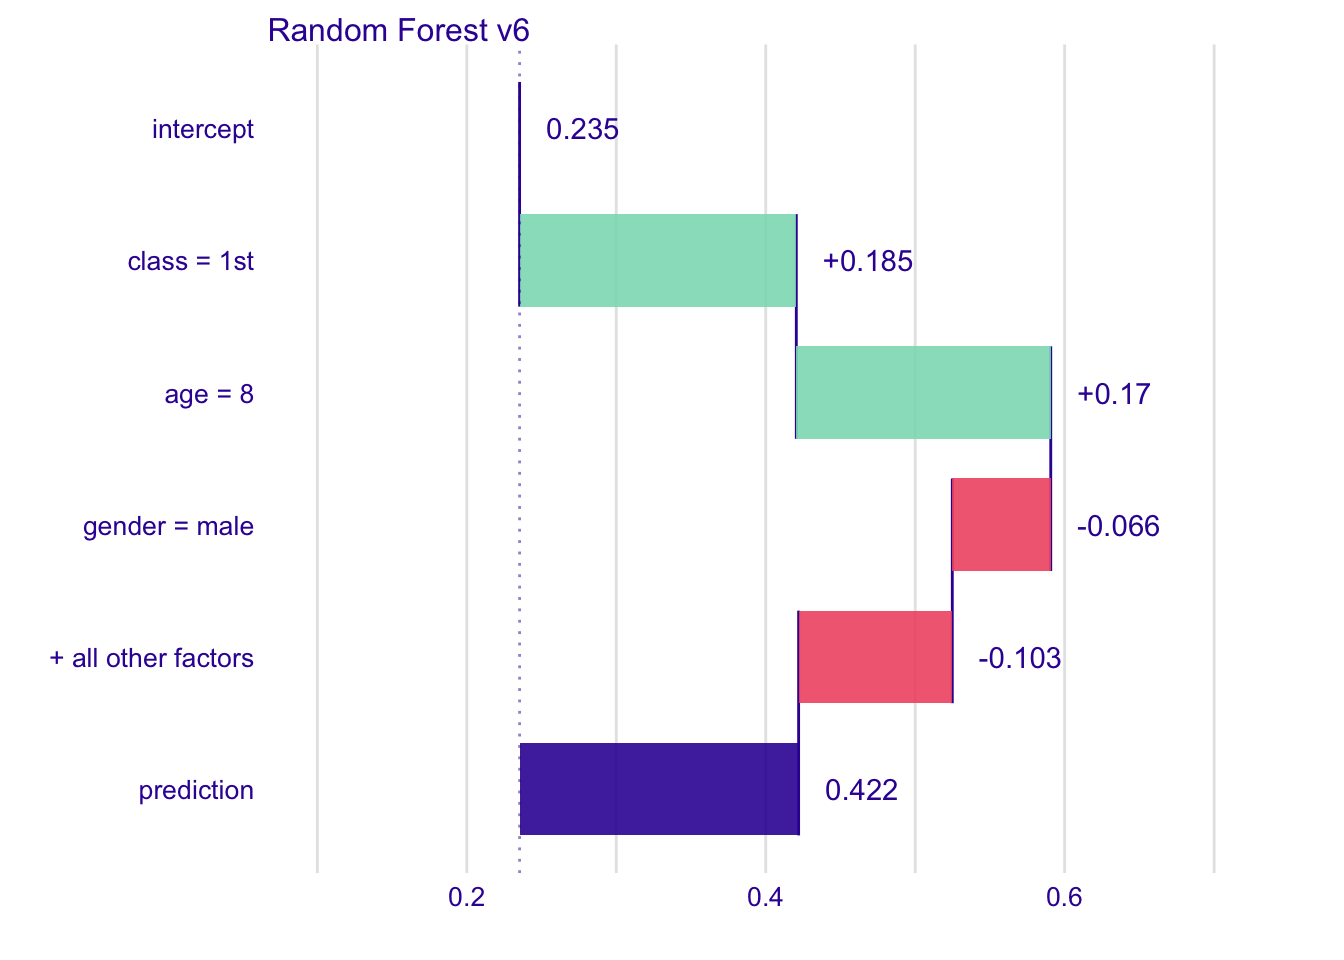
\includegraphics{PM_VEE_files/figure-latex/unnamed-chunk-34-1.pdf}

\textbf{Oscillations}

The \texttt{calculate\_oscillations()} function calculates oscillations
for CP profiles.

\begin{Shaded}
\begin{Highlighting}[]
\NormalTok{cp_rf_all <-}\StringTok{ }\KeywordTok{ceteris_paribus}\NormalTok{(explainer_rf, new_apartment)}
\NormalTok{co_rf_all <-}\StringTok{ }\KeywordTok{calculate_oscillations}\NormalTok{(cp_rf_all)}
\NormalTok{co_rf_all}
\end{Highlighting}
\end{Shaded}

\begin{verbatim}
##             _vname_ _ids_ oscillations
## 2           surface     1     651.8346
## 4          no.rooms     1     473.4988
## 3             floor     1     344.7220
## 1 construction.year     1     256.2264
\end{verbatim}

\begin{Shaded}
\begin{Highlighting}[]
\KeywordTok{plot}\NormalTok{(co_rf_all)}
\end{Highlighting}
\end{Shaded}

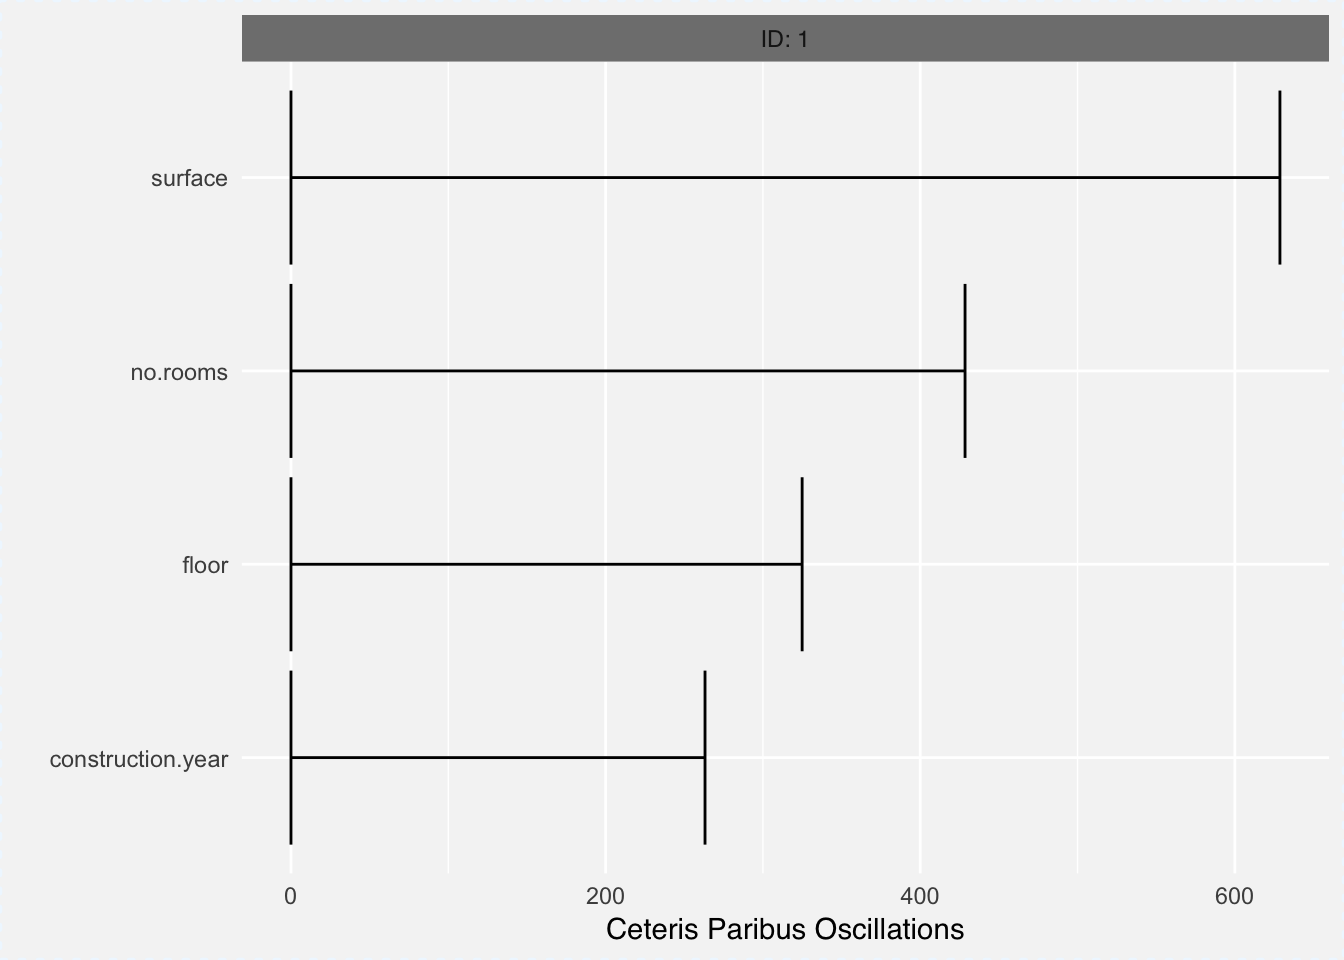
\includegraphics{PM_VEE_files/figure-latex/unnamed-chunk-35-1.pdf}

\textbf{2D Ceteris Paribus profiles}

And the \texttt{what\_if\_2d()} function calculates 2D CP profiles.

\begin{Shaded}
\begin{Highlighting}[]
\NormalTok{wi_rf_2d <-}\StringTok{ }\KeywordTok{what_if_2d}\NormalTok{(explainer_rf, }\DataTypeTok{observation =}\NormalTok{ new_apartment, }
                 \DataTypeTok{selected_variables =} \KeywordTok{c}\NormalTok{(}\StringTok{"surface"}\NormalTok{,}\StringTok{"floor"}\NormalTok{, }\StringTok{"construction.year"}\NormalTok{))}
\KeywordTok{plot}\NormalTok{(wi_rf_2d, }\DataTypeTok{split_ncol =} \DecValTok{2}\NormalTok{)}
\end{Highlighting}
\end{Shaded}

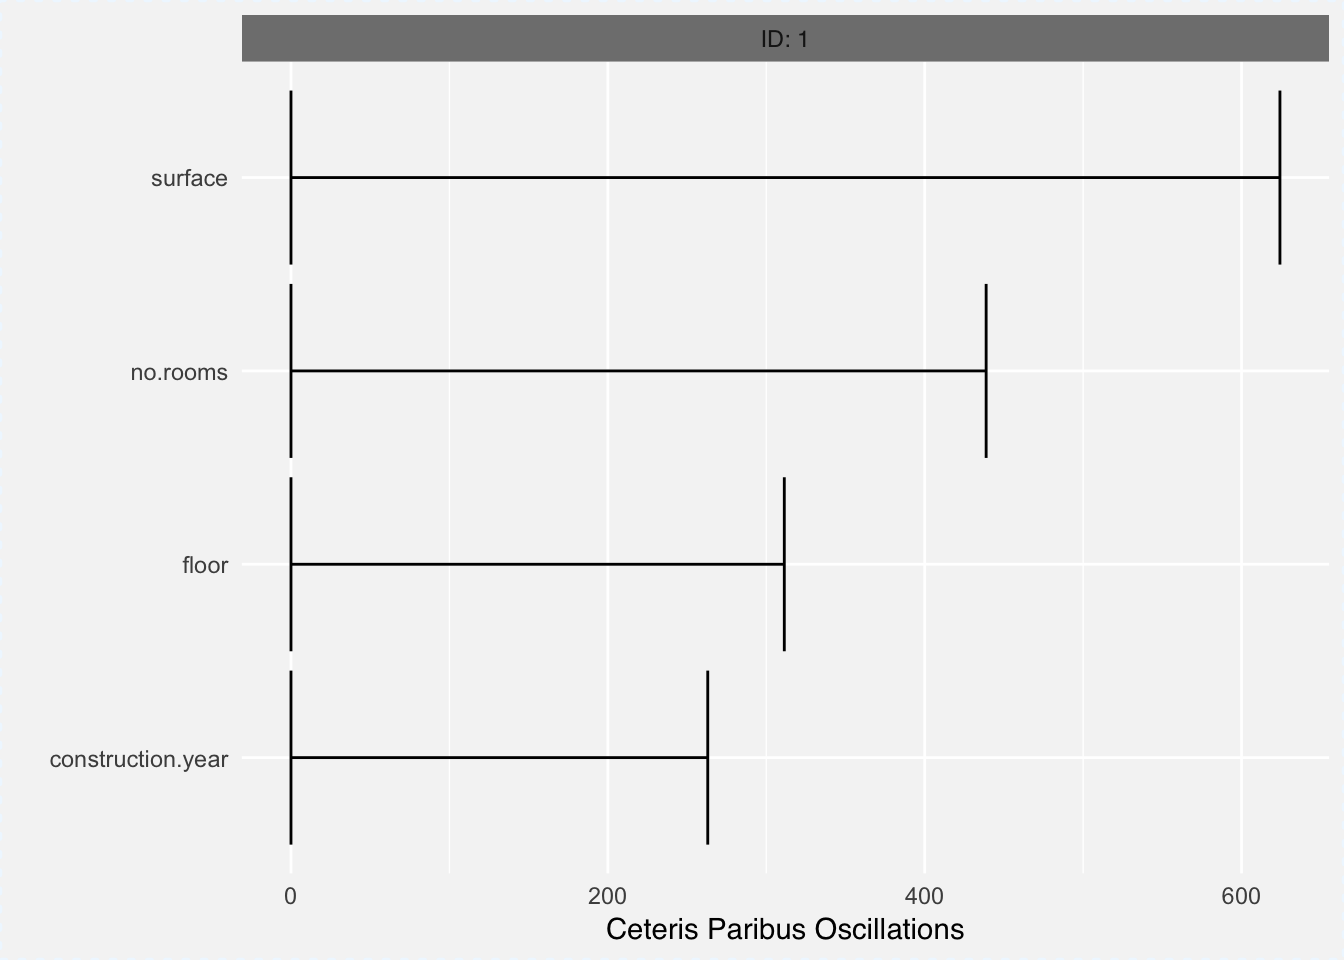
\includegraphics{PM_VEE_files/figure-latex/unnamed-chunk-36-1.pdf}

\hypertarget{model-level-explanations}{%
\chapter*{Model level explanations}\label{model-level-explanations}}
\addcontentsline{toc}{chapter}{Model level explanations}

\hypertarget{introduction-2}{%
\chapter{Introduction}\label{introduction-2}}

\hypertarget{a-bit-of-philosophy}{%
\section{A bit of philosophy}\label{a-bit-of-philosophy}}

Rights:

\begin{enumerate}
\def\labelenumi{\arabic{enumi}.}
\tightlist
\item
  audit model residuals
\item
  variable importance
\item
  partial dependency plot
\end{enumerate}

\hypertarget{example-price-prediction}{%
\section{Example: Price prediction}\label{example-price-prediction}}

\citep{R-DALEX}

\citep{R-e1071}

\citep{R-factorMerger}

\begin{Shaded}
\begin{Highlighting}[]
\KeywordTok{library}\NormalTok{(}\StringTok{"factorMerger"}\NormalTok{)}
\end{Highlighting}
\end{Shaded}

In this chapter we show examples for three predictive models trained on
\texttt{apartments} dataset from the \texttt{DALEX} package. Random
Forest model (elastic but biased), Support Vector Machines model (large
variance on boundaries) and Linear Model (stable but not very elastic).
Presented examples are for regression (prediction of square meter
price), but the CP profiles may be used in the same way for
classification.

\begin{Shaded}
\begin{Highlighting}[]
\KeywordTok{library}\NormalTok{(}\StringTok{"DALEX"}\NormalTok{)}
\CommentTok{# Linear model trained on apartments data}
\NormalTok{model_lm <-}\StringTok{ }\KeywordTok{lm}\NormalTok{(m2.price }\OperatorTok{~}\StringTok{ }\NormalTok{construction.year }\OperatorTok{+}\StringTok{ }\NormalTok{surface }\OperatorTok{+}\StringTok{ }\NormalTok{floor }\OperatorTok{+}\StringTok{ }
\StringTok{                      }\NormalTok{no.rooms }\OperatorTok{+}\StringTok{ }\NormalTok{district, }\DataTypeTok{data =}\NormalTok{ apartments)}

\KeywordTok{library}\NormalTok{(}\StringTok{"randomForest"}\NormalTok{)}
\KeywordTok{set.seed}\NormalTok{(}\DecValTok{59}\NormalTok{)}
\CommentTok{# Random Forest model trained on apartments data}
\NormalTok{model_rf <-}\StringTok{ }\KeywordTok{randomForest}\NormalTok{(m2.price }\OperatorTok{~}\StringTok{ }\NormalTok{construction.year }\OperatorTok{+}\StringTok{ }\NormalTok{surface }\OperatorTok{+}\StringTok{ }\NormalTok{floor }\OperatorTok{+}\StringTok{ }
\StringTok{                      }\NormalTok{no.rooms }\OperatorTok{+}\StringTok{ }\NormalTok{district, }\DataTypeTok{data =}\NormalTok{ apartments)}

\KeywordTok{library}\NormalTok{(}\StringTok{"e1071"}\NormalTok{)}
\CommentTok{# Support Vector Machinesr model trained on apartments data}
\NormalTok{model_svm <-}\StringTok{ }\KeywordTok{svm}\NormalTok{(m2.price }\OperatorTok{~}\StringTok{ }\NormalTok{construction.year }\OperatorTok{+}\StringTok{ }\NormalTok{surface }\OperatorTok{+}\StringTok{ }\NormalTok{floor }\OperatorTok{+}\StringTok{ }
\StringTok{                         }\NormalTok{no.rooms }\OperatorTok{+}\StringTok{ }\NormalTok{district, }\DataTypeTok{data =}\NormalTok{ apartments)}
\end{Highlighting}
\end{Shaded}

For these models we use \texttt{DALEX} explainers created with
\texttt{explain()} function. There exapliners wrap models, predict
functions and validation data.

\begin{Shaded}
\begin{Highlighting}[]
\NormalTok{explainer_lm <-}\StringTok{ }\KeywordTok{explain}\NormalTok{(model_lm, }
                       \DataTypeTok{data =}\NormalTok{ apartmentsTest[,}\DecValTok{2}\OperatorTok{:}\DecValTok{6}\NormalTok{], }\DataTypeTok{y =}\NormalTok{ apartmentsTest}\OperatorTok{$}\NormalTok{m2.price)}
\NormalTok{explainer_rf <-}\StringTok{ }\KeywordTok{explain}\NormalTok{(model_rf, }
                       \DataTypeTok{data =}\NormalTok{ apartmentsTest[,}\DecValTok{2}\OperatorTok{:}\DecValTok{6}\NormalTok{], }\DataTypeTok{y =}\NormalTok{ apartmentsTest}\OperatorTok{$}\NormalTok{m2.price)}
\NormalTok{explainer_svm <-}\StringTok{ }\KeywordTok{explain}\NormalTok{(model_svm, }
                       \DataTypeTok{data =}\NormalTok{ apartmentsTest[,}\DecValTok{2}\OperatorTok{:}\DecValTok{6}\NormalTok{], }\DataTypeTok{y =}\NormalTok{ apartmentsTest}\OperatorTok{$}\NormalTok{m2.price)}
\end{Highlighting}
\end{Shaded}

Examples presented in this chapter are generated with the
\texttt{ceterisParibus} package in version 0.3.1.

\begin{Shaded}
\begin{Highlighting}[]
\KeywordTok{library}\NormalTok{(}\StringTok{"ceterisParibus"}\NormalTok{)}
\end{Highlighting}
\end{Shaded}

\hypertarget{variable-importance}{%
\chapter{Variable Importance}\label{variable-importance}}

Feature selection

\citep{Strobl2007} \citep{Strobl2008} - variable importance

\citep{2018arXiv180101489F}

Beware Default Random Forest Importances

Terence Parr, Kerem Turgutlu, Christopher Csiszar, and Jeremy Howard
March 26, 2018.

\url{http://explained.ai/rf-importance/index.html}

\hypertarget{marginal-response}{%
\chapter{Marginal Response}\label{marginal-response}}

Feature extraction

\hypertarget{partial-dependency-plots}{%
\section{Partial Dependency Plots}\label{partial-dependency-plots}}

Accumulated Local Effects (ALE) Plots

\citep{RJ2017016} \citep{R-ALEPlot}

\begin{Shaded}
\begin{Highlighting}[]
\KeywordTok{library}\NormalTok{(ALEPlot)}
\end{Highlighting}
\end{Shaded}

\citep{MAGIX}

Interactions - extraction

\hypertarget{merging-path-plots}{%
\section{Merging Path Plots}\label{merging-path-plots}}

\citep{R-factorMerger}

\begin{Shaded}
\begin{Highlighting}[]
\KeywordTok{library}\NormalTok{(factorMerger)}
\end{Highlighting}
\end{Shaded}

\hypertarget{performance-diagnostic}{%
\chapter{Performance Diagnostic}\label{performance-diagnostic}}

Model selection

\hypertarget{residual-diagnostic}{%
\chapter{Residual Diagnostic}\label{residual-diagnostic}}

Model validation

\citep{R-auditor}

\begin{Shaded}
\begin{Highlighting}[]
\KeywordTok{library}\NormalTok{(auditor)}
\end{Highlighting}
\end{Shaded}

\hypertarget{other-topics}{%
\chapter{Other topics}\label{other-topics}}

\citep{R-randomForestExplainer} \citep{R-ICEbox} \citep{R-ALEPlot}

\begin{Shaded}
\begin{Highlighting}[]
\KeywordTok{library}\NormalTok{(randomForestExplainer)}
\KeywordTok{library}\NormalTok{(ICEbox)}
\KeywordTok{library}\NormalTok{(ALEPlot)}
\end{Highlighting}
\end{Shaded}

\citep{R-modelDown}

\begin{Shaded}
\begin{Highlighting}[]
\KeywordTok{library}\NormalTok{(modelDown)}
\end{Highlighting}
\end{Shaded}

\hypertarget{appendixes}{%
\chapter*{Appendixes}\label{appendixes}}
\addcontentsline{toc}{chapter}{Appendixes}

\hypertarget{DataSets}{%
\chapter{Data Sets}\label{DataSets}}

\hypertarget{HRdataset}{%
\section{Hire or Fire? HR in Call Center}\label{HRdataset}}

In this chapter we present an artificial dataset from Human Resources
department in a Call Center to present pros and cons for different
techniques of prediction level explainers.

The dataset is available in the \texttt{DALEX} package \citep{R-DALEX}.
Each row corresponds to a single employee of a call center. Features
like gender, age, average number of working hours per week, grade from
the last evaluation and level of salary are used as predictive features.

The problem here is to first build a model, that will determine when to
fires and when to promote an employer, so it's a classification problem
with three classes. But having a model we will use prediction level
explainers to better understand how the model works for selected cases.

\begin{Shaded}
\begin{Highlighting}[]
\KeywordTok{library}\NormalTok{(}\StringTok{"DALEX"}\NormalTok{)}
\KeywordTok{head}\NormalTok{(HR)}
\end{Highlighting}
\end{Shaded}

\begin{verbatim}
##   gender      age    hours evaluation salary   status
## 1   male 32.58267 41.88626          3      1    fired
## 2 female 41.21104 36.34339          2      5    fired
## 3   male 37.70516 36.81718          3      0    fired
## 4 female 30.06051 38.96032          3      2    fired
## 5   male 21.10283 62.15464          5      3 promoted
## 6   male 40.11812 69.53973          2      0    fired
\end{verbatim}

In this book we are focused on model exploration rather than model
building, thus for sake ok simplicity we will use two default models
created with random forest \citep{R-randomForest} and generalized linear
model \citep{R-nnet}.

\begin{Shaded}
\begin{Highlighting}[]
\KeywordTok{set.seed}\NormalTok{(}\DecValTok{59}\NormalTok{)}
\KeywordTok{library}\NormalTok{(}\StringTok{"randomForest"}\NormalTok{)}
\NormalTok{model_rf <-}\StringTok{ }\KeywordTok{randomForest}\NormalTok{(status }\OperatorTok{~}\StringTok{ }\NormalTok{gender }\OperatorTok{+}\StringTok{ }\NormalTok{age }\OperatorTok{+}\StringTok{ }\NormalTok{hours }\OperatorTok{+}\StringTok{ }\NormalTok{evaluation }\OperatorTok{+}\StringTok{ }\NormalTok{salary, }\DataTypeTok{data =}\NormalTok{ HR)}

\KeywordTok{library}\NormalTok{(}\StringTok{"nnet"}\NormalTok{)}
\NormalTok{model_glm <-}\StringTok{ }\KeywordTok{multinom}\NormalTok{(status }\OperatorTok{~}\StringTok{ }\NormalTok{gender }\OperatorTok{+}\StringTok{ }\NormalTok{age }\OperatorTok{+}\StringTok{ }\NormalTok{hours }\OperatorTok{+}\StringTok{ }\NormalTok{evaluation }\OperatorTok{+}\StringTok{ }\NormalTok{salary, }\DataTypeTok{data =}\NormalTok{ HR)}
\end{Highlighting}
\end{Shaded}

\begin{verbatim}
## # weights:  21 (12 variable)
## initial  value 8620.810629 
## iter  10 value 7002.127738
## iter  20 value 6239.478146
## iter  20 value 6239.478126
## iter  20 value 6239.478124
## final  value 6239.478124 
## converged
\end{verbatim}

\hypertarget{apartmentsDataset}{%
\section{How much does it cost? Price prediction for a square
meter}\label{apartmentsDataset}}

In this chapter we present an artificial dataset related to prediction
of prices for appartments in Warsaw. This dataset wil be used to discuss
pros and cons for different techniques of model level explainers.

The dataset is available in the \texttt{DALEX} package \citep{R-DALEX}.
Each row corresponds to a single apartment. Features like surface,
number of rooms, district or floor are used as predictive features.

The problem here is to predict price of a square meter for an
appartment, so it's a regression problem with continouse outcome.

\begin{Shaded}
\begin{Highlighting}[]
\KeywordTok{library}\NormalTok{(}\StringTok{"DALEX"}\NormalTok{)}
\KeywordTok{head}\NormalTok{(apartments)}
\end{Highlighting}
\end{Shaded}

\begin{verbatim}
##   m2.price construction.year surface floor no.rooms    district
## 1     5897              1953      25     3        1 Srodmiescie
## 2     1818              1992     143     9        5     Bielany
## 3     3643              1937      56     1        2       Praga
## 4     3517              1995      93     7        3      Ochota
## 5     3013              1992     144     6        5     Mokotow
## 6     5795              1926      61     6        2 Srodmiescie
\end{verbatim}

The problem here is to predict average price for square meter for an
apartment. Let's build a random forest model with \texttt{randomForest}
package \citep{R-randomForest}.

\begin{Shaded}
\begin{Highlighting}[]
\KeywordTok{library}\NormalTok{(}\StringTok{"randomForest"}\NormalTok{)}
\NormalTok{model_rf <-}\StringTok{ }\KeywordTok{randomForest}\NormalTok{(m2.price }\OperatorTok{~}\StringTok{ }\NormalTok{construction.year }\OperatorTok{+}\StringTok{ }\NormalTok{surface }\OperatorTok{+}\StringTok{ }\NormalTok{floor }\OperatorTok{+}\StringTok{ }\NormalTok{no.rooms }\OperatorTok{+}\StringTok{ }\NormalTok{district, }\DataTypeTok{data =}\NormalTok{ apartments)}
\NormalTok{model_rf}
\end{Highlighting}
\end{Shaded}

\begin{verbatim}
## 
## Call:
##  randomForest(formula = m2.price ~ construction.year + surface +      floor + no.rooms + district, data = apartments) 
##                Type of random forest: regression
##                      Number of trees: 500
## No. of variables tried at each split: 1
## 
##           Mean of squared residuals: 82079.37
##                     % Var explained: 90.01
\end{verbatim}

And a linear model.

\begin{Shaded}
\begin{Highlighting}[]
\NormalTok{model_lm <-}\StringTok{ }\KeywordTok{lm}\NormalTok{(m2.price }\OperatorTok{~}\StringTok{ }\NormalTok{construction.year }\OperatorTok{+}\StringTok{ }\NormalTok{surface }\OperatorTok{+}\StringTok{ }\NormalTok{floor }\OperatorTok{+}\StringTok{ }\NormalTok{no.rooms }\OperatorTok{+}\StringTok{ }\NormalTok{district, }\DataTypeTok{data =}\NormalTok{ apartments)}
\NormalTok{model_lm}
\end{Highlighting}
\end{Shaded}

\begin{verbatim}
## 
## Call:
## lm(formula = m2.price ~ construction.year + surface + floor + 
##     no.rooms + district, data = apartments)
## 
## Coefficients:
##         (Intercept)    construction.year              surface  
##            5020.139               -0.229              -10.238  
##               floor             no.rooms      districtBielany  
##             -99.482              -37.730               17.214  
##     districtMokotow       districtOchota        districtPraga  
##             918.380              926.254              -37.105  
## districtSrodmiescie        districtUrsus      districtUrsynow  
##            2080.611               29.942              -18.865  
##        districtWola     districtZoliborz  
##             -16.891              889.973
\end{verbatim}

\bibliography{book.bib,packages.bib}


\end{document}
